%&bericht

%%%%%%%%%%%%%%%%%%%%%%%%%%%%%%%%%%%%%%%%%%%%%%%%%%%%%%%%%%%%%%%%%%%%%%%%%%%%%%%
%% Descr:       Vorlage für Berichte der DHBW-Karlsruhe
%% Author:      Prof. Dr. Jürgen Vollmer, juergen.vollmer@dhbw-karlsruhe.de
%% $Id: bericht.tex,v 1.25 2020/03/13 15:07:45 vollmer Exp $
%%  -*- coding: utf-8 -*-
%%%%%%%%%%%%%%%%%%%%%%%%%%%%%%%%%%%%%%%%%%%%%%%%%%%%%%%%%%%%%%%%%%%%%%%%%%%%%%%

\documentclass[
   ngerman          % neue deutsche Rechtschreibung
  ,a4paper          % Papiergrösse
% ,twoside          % Zweiseitiger Druck (rechts/links)
% ,10pt             % Schriftgrösse
  ,11pt
% ,12pt
  ,pdftex
%  ,disable         % Todo-Markierungen auschalten
]{report}

% Bitte die Codierung Ihrer Dateien auswählen:
% \usepackage[latin1]{inputenc}    % Für UNIX mit ISO-LATIN-codierten Dateien
% \usepackage[applemac]{inputenc}  % Für Apple Mac
% \usepackage[ansinew]{inputenc}   % Für Microsoft Windows
\usepackage[utf8]{inputenc}        % UTF-8 codierte Dateien
                                   % Dieses Dokument ist unter Unix erstellt, daher
                                   % wird diese Input-Codierung benutzt.
\setlength{\marginparwidth}{2cm}
\usepackage{bericht}
\usepackage{makecell}

%% ACHTUNG, wenn man eine eigene Formatdatei (bericht.fmt) benutzt, werden Änderungen an bericht.sty
%% erst wirksam, wenn die Format-Datei neu erzeugt wurde!!!
%% Genauer alle Änderungen, die textuell vor der nächsten Zeile ".... endofdump...." stehen
%% werden erst wirksam, wenn die Formatdatei neu erzeugt wurde
\csname endofdump\endcsname

%%listing settings
\lstset{showstringspaces=false}

%%%%%%%%%%%%%%%%%%%%%%%%%%%%%%%%%%%%%%%%%%%%%%%%%%%%%%%%%%%%%%%%%%%%%%%%%%%%%%%
%% Angaben zur Arbeit
%%%%%%%%%%%%%%%%%%%%%%%%%%%%%%%%%%%%%%%%%%%%%%%%%%%%%%%%%%%%%%%%%%%%%%%%%%%%%%%

\newcommand{\Autor}{Felix Manuel Gervasi}
\newcommand{\AutorZwei}{Alena Sutiagina}
\newcommand{\MatrikelNummerFelix}{1052491 (Gervasi)}
\newcommand{\MatrikelNummerAlena}{6235629 (Sutiagina)}
\newcommand{\Kursbezeichnung}{TINF20B4}

\newcommand{\FirmenName}{}
\newcommand{\FirmenStadt}{}
\newcommand{\FirmenLogoDeckblatt}{}

% Falls es kein Firmenlogo gibt:
%  \newcommand{\FirmenLogoDeckblatt}{}

\newcommand{\BetreuerFirma}{Prof. Dr. Jörn Eisenbiegler}

%%%%%%%%%%%%%%%%%%%%%%%%%%%%%%%%%%%%%%%%%%%%%%%%%%%%%%%%%%%%%%%%%%%%%%%%%%%%%%%%%%%%%

% Wird auf dem Deckblatt und in der Erklärung benutzt:
\newcommand{\Was}{Studienarbeit}

%%%%%%%%%%%%%%%%%%%%%%%%%%%%%%%%%%%%%%%%%%%%%%%%%%%%%%%%%%%%%%%%%%%%%%%%%%%%%%%%%%%%%

\newcommand{\Titel}{Bedienung einer Getränkemischmaschine über Sprachbefehle}
\newcommand{\AbgabeDatum}{22. Mai 2023}

\newcommand{\Dauer}{6 Monate}

\newcommand{\Abschluss}{Bachelor of Science}

\newcommand{\Studiengang}{Angewandte Informatik}

\hypersetup{%%
  pdfauthor={\Autor},
  pdftitle={\Titel},
  pdfsubject={\Was}
}

% um die nervigen Errors zu eliminieren, die auftauchen, wenn man versucht
% einen Zeilenumbruch manuell innerhalb eines section-Titels einzufügen
% s. https://tex.stackexchange.com/questions/10555/hyperref-warning-token-not-allowed-in-a-pdf-string
\pdfstringdefDisableCommands{%
  \def\\{}%
}

%%%%%%%%%%%%%%%%%%%%%%%%%%%%%%%%%%%%%%%%%%%%%%%%%%%%%%%%%%%%%%%%%%%%%%%%%%%%%%%

% Wenn \includeonly{..} benutzt wird, werden nur diese Kaptitel ausgegeben.
%\includeonly{
%  abk
% ,kapitel1
% ,kapitel2
% ,changelog
%}

%%%%%%%%%%%%%%%%%%%%%%%%%%%%%%%%%%%%%%%%%%%%%%%%%%%%%%%%%%%%%%%%%%%%%%%%%%%%%%%

% Benutzt man das "biblatex"-Paket, dann muß das hier stehen:
% siehe auch die mit BIBLATEX markierten Zeilen in bericht.sty
\bibliography{bericht}

\graphicspath{{img/}}

\begin{document}

%%%%%%%%%%%%%%%%%%%%%%%%%%%%%%%%%%%%%%%%%%%%%%%%%%%%%%%%%%%%%%%%%%%%%%%%%%%%%%%

\begin{titlepage}
  \begin{center}
    \vspace*{-2cm}
    \FirmenLogoDeckblatt\hfill
\includegraphics[width=4cm]{DHBW_Logo_KA}\\[2cm]
    {\Huge \Titel}\\[1cm]
    {\Huge\scshape \Was}\\[1cm]
    {\large für die Prüfung zum}\\[0.5cm]
    {\Large \Abschluss}\\[0.5cm]
    {\large des Studienganges \Studiengang}\\[0.5cm]
    {\large an der}\\[0.5cm]
    {\large Dualen Hochschule Baden-Württemberg Karlsruhe}\\[0.5cm]
    {\large von}\\[0.5cm]
    {\large\bfseries \Autor}\\[0.5cm]
    {\large und}\\[0.5cm]
    {\large\bfseries \AutorZwei}\\[1cm]
    {\large Abgabedatum \AbgabeDatum}
    \vfill
  \end{center}
  \begin{tabular}{l@{\hspace{2cm}}l}
    Bearbeitungszeitraum       & \Dauer               \\
    Matrikelnummer             & \MatrikelNummerFelix \\
                               & \MatrikelNummerAlena \\
    Kurs                       & \Kursbezeichnung     \\
    Betreuer der Studienarbeit & \BetreuerFirma       \\
  \end{tabular}
\end{titlepage}

%%%%%%%%%%%%%%%%%%%%%%%%%%%%%%%%%%%%%%%%%%%%%%%%%%%%%%%%%%%%%%%%%%%%%%%%%%%%%%%

%%%%%%%%%%%%%%%%%%%%%%%%%%%%%%%%%%%%%%%%%%%%%%%%%%%%%%%%%%%%%%%%%%%%%%%%%%%%%%%
%% Descr:       Vorlage für Berichte der DHBW-Karlsruhe, Erklärung
%% Author:      Prof. Dr. Jürgen Vollmer, vollmer@dhbw-karlsruhe.de
%% $Id: erklaerung.tex,v 1.11 2020/03/13 14:24:42 vollmer Exp $
%% -*- coding: utf-8 -*-
%%%%%%%%%%%%%%%%%%%%%%%%%%%%%%%%%%%%%%%%%%%%%%%%%%%%%%%%%%%%%%%%%%%%%%%%%%%%%%%

% In Bachelorarbeiten muss eine schriftliche Erklärung abgegeben werden.
% Hierin bestätigen die Studierenden, dass die Bachelorarbeit, etc.
% selbständig verfasst und sämtliche Quellen und Hilfsmittel angegeben sind. Diese Erklärung
% bildet das zweite Blatt der Arbeit. Der Text dieser Erklärung muss auf einer separaten Seite
% wie unten angegeben lauten.

\newpage
\thispagestyle{empty}
\begin{framed}
\begin{center}
\Large\bfseries Erklärung
\end{center}
\medskip
\noindent
% siehe §5(3) der \enquote{Studien- und Prüfungsordnung DHBW Technik} vom 29.\,9.\,2017 und Anhang 1.1.13
Ich versichere hiermit, dass ich meine \Was mit dem Thema:
\enquote{\Titel}
selbstständig verfasst und keine anderen als die angegebenen Quellen und Hilfsmittel benutzt habe. Ich versichere zudem, dass die eingereichte elektronische Fassung mit der gedruckten Fassung übereinstimmt.
\vspace{3cm} \\
\underline{\hspace{4cm}}\hfill\underline{\hspace{6cm}}\\
Ort~~~~~Datum\hfill Unterschrift\hspace{4cm}
\end{framed}

%%%%%%%%%%%%%%%%%%%%%%%%%%%%%%%%%%%%%%%%%%%%%%%%%%%%%%%%%%%%%%%%%%%%%%%%%%%%%%%
\endinput
%%%%%%%%%%%%%%%%%%%%%%%%%%%%%%%%%%%%%%%%%%%%%%%%%%%%%%%%%%%%%%%%%%%%%%%%%%%%%%%


%%%%%%%%%%%%%%%%%%%%%%%%%%%%%%%%%%%%%%%%%%%%%%%%%%%%%%%%%%%%%%%%%%%%%%%%%%%%%%%

\begin{abstract}
  Ziel der Arbeit ist die Implementierung einer Sprachsteuerung für eine Mischmaschine, die Getränke zu unterschiedlichen Mischungsverhältnissen aus vier verschiedenen Behältern mischen kann. Die Mischmaschine soll dabei nicht nur die Sprache des Benutzers erkennen und daraufhin Aktionen durchführen sondern auch Antworten, sodass eine Art von Dialog zwischen Mischmaschine und Benutzer entsteht. Um das Ziel zu erreichen werden zunächst die theoretischen und technischen Grundlagen erarbeitet, wobei insbesondere auf die Verarbeitung von Sprache mit Hilfe von Künstlicher Intelligenz eingegangen wird. Anschließend werden die Anforderungen an das Projekt konkretisiert. Verschiedene Konzepte werden vorgestellt und evaluiert. Ein Konzept sieht vor zur Implementierung der Sprachsteuerung ausschließlich die bereits in der Mischmaschine verbaute Hardware zu verwenden. Ein weiteres Konzept sieht die Benutzung einer mobilen Anwendung vor, um die vorhandenen Rechenkapazitäten zu erweitern. Das dritte Konzept erklärt, wie Computer-Hardware eingesetzt werden kann, um die Sprachsteuerung zu implementieren. Außerdem werden verschiedene Ansätze für das Dialogsystem diskutiert. Es wird erläutert warum die Wahl für die Implementierung schließlich auf das soeben genannte, dirtte Konzept fällt. Ergebnis der Arbeit ist eine Sprachsteuerung für die Mischmaschine, die mit Hilfe eines Raspberry Pi 4 Modell B in Kombination mit dem, in der Mischmaschine verbauten, Arduino Mega funktioniert. Der Benutzer hat die Möglichkeit über ein Mikrofon, das an den Raspberry Pi angeschlossen ist, mit der Maschine zu kommunizieren. Die über das Mikrofon aufgenommenen Audisognale werden zunächst in Text konvertiert. Der Text wird von einem Sprachmodell interpretiert und klassifiziert. Ergebnis der Interpretation sind ein, für die Mischmaschine verständliches Kommando und die auszugebende Antwort. Das Kommando wird über eine serielle Schnittstelle vom Raspberry Pi an den Ardunino übertragen, der die Mischmaschine steuert. Die Mischmaschine führt daraufhin die gewünschte Aktion aus und der Raspberry Pi gibt die Antwort über Lautsprecher an den Benutzer zurück.
\end{abstract}

\renewcommand{\abstractname}{Abstract}
\begin{abstract}
  The goal of this paper is the implementation of a voice control for a mixing machine that can mix beverages with different mixing ratios from four different containers. The mixing machine should not only recognize the user's speech and perform actions on it, but also answer, so that a kind of dialog between mixing machine and user is created. To achieve this goal, the theoretical and technical basics are worked out, especially the processing of speech with the help of artificial intelligence. Subsequently, the requirements for the project will be specified. Different concepts are presented and evaluated. A concept is to use only the hardware already installed in the mixing machine to implement the voice control. Another concept envisages the use of a mobile
  application to extend the existing computing capacity. The third concept explains how computer hardware can be used to implement voice control. Different approaches to the dialog system are also discussed. It is explained why the choice for the implementation finally falls on the just mentioned, third concept for the implementation. The result of the work is a voice control for the mixing machine, which is implemented using a
  Raspberry Pi 4 model B in combination with the Arduino Mega, which is installed in the mixing machine. The user has the possibility to communicate with the mixing machine via a microphone that is connected to the Raspberry Pi, to communicate with the machine. The audio signals are first converted into text. The text is interpreted and classified by a speech model. The result of the interpretation is a command that can be understood by the mixing machine and the response to be output. The command is sent via
  serial interface from the Raspberry Pi to the Ardunino, which controls the mixing machine. The mixing machine then executes the desired action and the Raspberry Pi
  returns the response to the user via loudspeaker.
\end{abstract}

\newpage
\pagenumbering{roman}
\newcounter{roman-numbering}
\tableofcontents           % Inhaltsverzeichnis hier ausgeben
\clearpage
\addcontentsline{toc}{chapter}{Abbildungsverzeichnis}
\listoffigures             % Liste der Abbildungen
\clearpage
\addcontentsline{toc}{chapter}{Tabellenverzeichnis}
\listoftables              % Liste der Tabellen
\clearpage
\addcontentsline{toc}{chapter}{Listingverzeichnis}
\lstlistoflistings         % Liste der Listings
\clearpage
\addcontentsline{toc}{chapter}{Formelverzeichnis}
\listofequations           % Liste der Formeln

% Jetzt kommt der "eigentliche" Text
%%%%%%%%%%%%%%%%%%%%%%%%%%%%%%%%%%%%%%%%%%%%%%%%%%%%%%%%%%%%%%%%%%%%%%%%%%%%%%
%% Descr:       Vorlage für Berichte der DHBW-Karlsruhe, Datei mit Abkürzungen
%% Author:      Prof. Dr. Jürgen Vollmer, vollmer@dhbw-karlsruhe.de
%% $Id: abk.tex,v 1.4 2017/10/06 14:02:03 vollmer Exp $
%% -*- coding: utf-8 -*-
%%%%%%%%%%%%%%%%%%%%%%%%%%%%%%%%%%%%%%%%%%%%%%%%%%%%%%%%%%%%%%%%%%%%%%%%%%%%%%%

\chapter*{Abkürzungsverzeichnis}                   % chapter*{..} -->   keine Nummer, kein "Kapitel"
						         % Nicht ins Inhaltsverzeichnis
\addcontentsline{toc}{chapter}{Akürzungsverzeichnis}   % Damit das doch ins Inhaltsverzeichnis kommt

% Hier werden die Abkürzungen definiert
\begin{acronym}[BIS]
  % \acro{Name}{Darstellung der Abkürzung}{Langform der Abkürzung}
 \acro{Abk}[Abk.]{Abkürzung}

 % Folgendes benutzen, wenn der Plural einer Abk. benöigt wird
 % \newacroplural{Name}{Darstellung der Abkürzung}{Langform der Abkürzung}
 \newacroplural{Abk}[Abk-en]{Abkürzungen}

 \acro{H2O}[\ensuremath{H_2O}]{Di-Hydrogen-Monoxid}

 % Wenn neicht benutzt, erscheint diese Abk. nicht in der Liste
 \acro{NUA}{Not Used Acronym}
 \acro{HTTP}{Hypertext Transfer Protocol}
 \acro{NLP}{Natural Language Processing}
 \acro{AIML}{Artificial Intelligence Markup Language}
 \acro{XML}{eXtensible Markup Language}
 \acro{NLTK}{Natural Language Toolkit}
 \acro{TF}{Term Frequency}
 \acro{IDF}{Inverse Document Frequency}
 \acro{RBM}{Restricted Boltzmann Machines}
 \acro{GAN}{Generative Adversarial Network}
 \acro{RNN}{Recurrent Neural Networks}
 \acro{IoT}{Internet der Dinge}
 \acro{KI}{Künstlichen Intelligenz}
 \acro{ML}{Machine Learning}
 \acro{UI}{User Interface}
 \acro{RAM}{Read Only Memory}
 \acro{CFG}{Context-free grammar}
 \acro{NLTK}{Natural Language Toolkit}
 \acro{API}{Application Programming Interface}
 \acro{CMU}{Carnegie Mellon University}
 \acro{BOW}{Bag Of Words}
 \acro{seq2seq}{sequence-to-sequence}
 \acro{GB}{Gigabyte}
 \acro{TF-IDF}{Term Frequency-Inverse Document Frequency}
 \acro{MLP}{Multilayer Perceptron}
 \acro{LSA}{Latent Semantic Analysis}
 \acro{SWZ}{Singulärwertzerlegung}
 \acro{SVD}{Singular Value Decomposition}
 \acro{MLP}{Mehrschichtiges Perzeptron}
\end{acronym}

              % Abkürzungsverzeichnis
\setcounter{roman-numbering}{\value{page}}
\pagenumbering{arabic}
\chapter{Einleitung}
% Einführung: Interesse vom Leser wecken
Die Informationstechnik versteckt sich heutzutage fast überall - selbst dort, wo sie von den meisten Menschen nicht vermutet werden würde. Beispiele hierfür sind Autos, Kaffeemaschinen, Zahnbürsten, Rasierer, Küchengeräte und vieles mehr. Grund dafür ist die fortschreitende Möglichkeit der Miniaturisierung von Computern, sodass diese nahezu überall verbaut werden können. Beispielsweise können Mikrochips in der Kaffeemaschine dafür sorgen, dass die richtige Menge an Kaffee serviert wird oder der Füllstand der einzelnen Behälter angezeigt werden kann. Solche Systeme, die Informationen mit Hilfe eines Computers verarbeiten und dabei mit ihrer Umgebung derartig \glqq{}verschmelzen\grqq{}, nennt man auch \textit{embedded systems} (z. Dt. \textit{eingebettete Systeme}) \cite{marwedel_eingebettete_2021}.\\\\
Der aktuelle Trend des \ac{IoT} führt zu einem noch größeren Anstieg eingebetteter Systeme im Alltag. Im \ac{IoT} geht es speziell um eingebettete Systeme, die internetfähig (vernetzt) sind. Nach Schätzungen des Marktforschungsunternehmens \textit{Gartner} gab es im Jahr 2017 8,4 Milliarden solcher vernetzten Geräte weltweit \cite{jansen_digitalisierung_2017}. Das die Menge der vernetzten Geräte als Teilmenge der eingebetteten Systeme betrachtet werden kann ist damit zu rechnen, dass deren Anzahl sogar weit größer ausfällt.

\section{Aufgabenstellung}
Im Rahmen dieser Arbeit geht es um die Sprachsteuerung einer Getränkemischmaschine, die in diesem Fall als eingebettetes System zu verstehen ist und in einer vorangegangenen Arbeit bereits konzipiert und gebaut wurde \cite{mischmaschine}. Sie verfügt derzeit über ein Touch-Display zur Bedienung durch den Benutzer. Ziel der Arbeit ist es zusätzlich eine natürlichsprachliche Interaktion mit der Maschine zu ermöglichen, die mindestens den Funktionsumfang besitzt, der aktuell über die Bildschirmeingabe möglich ist. Dabei soll die Maschine nicht nur in der Lage sein die natrüliche Sprache des Benutzers in ein geeignetes Format umzuwandeln, sodass die Maschine den korrekten Befehl ausführt. Sie soll auch in der Lage sein dem Benutzer zu Antworten, sodass die Illusion einer Konversation mit der Maschine entsteht.

\section{Vorgehen}
Zunächst müssen die Sprachverarbeitung und Spracherkennung betrachtet werden. Die Sprachverarbeitung dient der Interpretation des Gesprochenen um eine geeignete Antwort auszugeben und dem Übersetzen in einen Maschinenbefehl. Im Rahmen dieser Arbeit sollen dafür Verfahren und Techniken der \ac{KI} und des \ac{ML} eingesetzt werden. Die Spracherkennung beschäftigt sich mit der Aufnahme des Tonsignals bzw. der Schallwellen (bspw. über ein Mikrofon) und dem Umwandeln dieser Signale in Text, sodass dieser an das \ac{KI}-Modell weitergereicht werden kann.\\\\
Bei der Arbeit mit eingebetteten Systemen muss man sich der vorhandenen Hardwareleistung und den benötigten Hardwareanforderungen bewusst sein, da diese meist sehr begrenzt ist. Deshalb werden im Rahmen dieser Arbeit verschiedene Ansätze diskutiert, wie und wo die einzelnen Schritte und Berechnungen ablaufen sollen (s. Kapitel \ref{chap:konzept}).
\endinput
\chapter{Theoretische und technische Grundlagen}
Dieses Kapitel beschäftigt sich mit der Erarbeitung theoretischer und technischer Grundlagen die im weiteren Verlauf der Arbeit angewendet wurden.
\section{Getränkemischmaschine}
Ziel dieser Arbeit ist die Implementierung einer Sprachsteuerung für eine Getränkemischmaschine. Die Getränkemischmaschine wurde bereits in einem vorangegangenen Projekt erstellt \cite{mischmaschine}. In diesem Abschnitt wird darauf eingegangen, um was für eine Art von Maschine es sich dabei handelt und es werden ihre Funktionsweise und ihr Aufbau beschrieben.\\\\
Das Mischen von Getränken bzw. Flüssigkeiten ist der Anwendungsfall für den die Maschine konzipiert wurde. Dazu besitzt die Mischmaschine fünf Behälter zu je einem Liter. Jedem Behälter ist eine Pumpe zugeordnet, die separat angesteuert werden kann und dafür sorgt, dass die Flüssigkeit aus dem Behälter zur Getränkeausgabe gelangt. Kurz vor dem Ausgang werden die Schläuche der Behälter zusammengeführt, wodurch letztlich die Mischung der verschiedenen Getränke erzielt wird. Sogenannte \glqq{}Rückschlagventile\grqq{} sorgen dafür, dass ein Zurückfließen der Getränkemischung in die Behälter verhindert wird.\\\\
Zur Steuerung der Maschine durch einen Benutzer befinden sich an der Vorderseite zwei Knöpfe und ein Touch-Display. Einer der Knöpfe dient dem Anschalten der Maschine und ein weiterer der Ausgabe des Getränks. Über das Touch-Display kann der Benutzer die Mischung seiner Getränke konfigurieren und die Maschine administrieren.\\\\
\begin{figure}[H]
    \centering
    \fbox{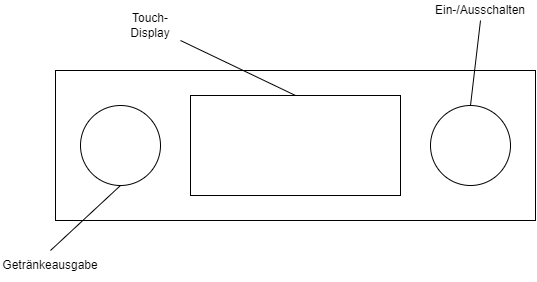
\includegraphics[width=0.8\textwidth]{img/Bilder_Stand_der_Technik/Bedienungsschnittstelle_Mischmaschine.png}}
    \caption{Schematischer Aufbau der Bedienungsschnittstelle}
    \label{fig:bedienungsschnittstelle_mischmaschine}
\end{figure}
\noindent
Abbildung \ref{fig:bedienungsschnittstelle_mischmaschine} stellt den schematischen Aufbau der Bedienungsschnittstelle der Getränkemischmaschine für ein besseres Verständnis dar.\\\\
Die technische Umsetzung basiert auf der Kommunikation zwischen dem Touch-Display und einem, in der Getränkemischmaschine verbauten, Arduino, der anhand der Daten von der Benutzereingabe, die Pumpen steuert. Beim Drücken des Startknopfes werden das Display und der Arduino mit Strom versorgt, sodass sowohl das Display als auch der Arduino starten und mit der Ausführung des benutzerdefinierten Quelltextes beginnen. Auf dem Bediendisplay finden sich fünf Schieberegler - ein Schieberegler je Behälter - mit denen der Benutzer die Zusammensetzung seines Mischgetränks aus den fünf Behältern konfigurieren kann. Beim Drücken eines in der \ac{UI} des Displays dargestellten Knopfes werden die Werte der Schieberegler an den Arduino übertragen. Dieser rechnet die Prozentwerte der Schieberegler in Durchsatzraten für die Pumpen um. Wird anschließend der Knopf für die Getränkeausgabe gedrückt gehalten steuert der Arduino die Pumpen mit ihrer jeweiligen Durchsatzrate an und der Anwender bekommt sein Mischgetränk ausgegeben.\\\\
Neben den bereits genannten Komponenten besitzt die Mischmaschine außerdem einen Wasserstandssensor je Behälter, um ein Trockenlaufen der Pumpen zu verhindern. Wie die einzelnen Komponenten zusammenspielen ist in dem Anhang \ref{Anhang_D} zu sehen, der den schematischen Aufbau/Schaltplan der Getränkemischmaschine zeigt \cite{mischmaschine}.
\section{Hardware}
\subsection{Arduino}
\subsubsection{Allgemeines}
Arduino ist eine Plattform/Organisation, die sich der Herstellung von Mikrocontrollern und der für den Umgang mit der Hardware erforderlichen Software widmet. Darunter fallen in erster Linie die Arduino-IDE und -Sprache zur Programmierung der Arduino-Mikrocontroller. Arduino verfolgt das Ziel, Hardwareprogrammierung oder \ac{IT} im Allgemeinen für alle Menschen unabhängig ihres Hintergrunds zu ermöglichen und näher zu bringen - allen voran auch denjenigen, die sich nicht professionell mit \ac{IT} auseinandersetzen \cite{arduino_education}. Deshalb liegt der Fokus von Arduino auf preisgünstigen Mikrocontrollern und einer einfachen Handhabung. Arduino stellt zu diesem Zweck auch viele Lernmaterialien bereit, die bspw. von Lehrkräften verwendet werden können als auch eine Community-Plattform für den Wissensaustausch zwischen den Benutzern von Arduino Hard- und Software. Pläne für die Arduino-Boards werden unter der \textit{Creative Commons} Lizenz veröffentlicht, sodass sie von anderen nachgebaut oder erweitert werden können. Auch der Quelltext der Arduino-Software ist quelloffen.\\\\
Aufgrund des großen Erfolgs von Arduino gibt es inzwischen zahlreiche Nachahmungen wie bspw. ...
\subsubsection{Arduino-Programmierung}
Die Programmierung eines Arduino-Mikrocontrollers erfolgt über die Arduino-IDE. Die Arduino-IDE kann auf allen gängigen Betriebssystemen (Windows, Mac und Linux) installiert und verwendet werden, was den Umgang mit Arduino sehr flexibel und gut für Einsteiger macht, da sie ihre gewohnte Umgebung verwenden können. Die Arduino-IDE ist dabei angelehnt an andere, gängige Entwicklungsumgebungen, sodass sich erfahrene Programmierer sofort zurecht finden, ist aber auf die Arduino-Programmierung optimiert. Beispielsweise werden an den Computer angeschlossene Boards automatisch erkannt, per Knopfdruck kann der aktuelle Quelltext auf den Mikrocontroller hochgeladen werden und die evtl. zusätzlich benötigten C++-Bibliotheken können verwaltet werden. Neben der Desktop-Version kann die Arduino-Entwicklungsumgebung auch online im Browser verwendet werden. Abbildung \ref{img:arduino_ide} zeigt einen Ausschnitt der Benutzeroberfläche in der Arduino-Entwicklungsumgebung.
\begin{figure}[H]
    \centering
    \fbox{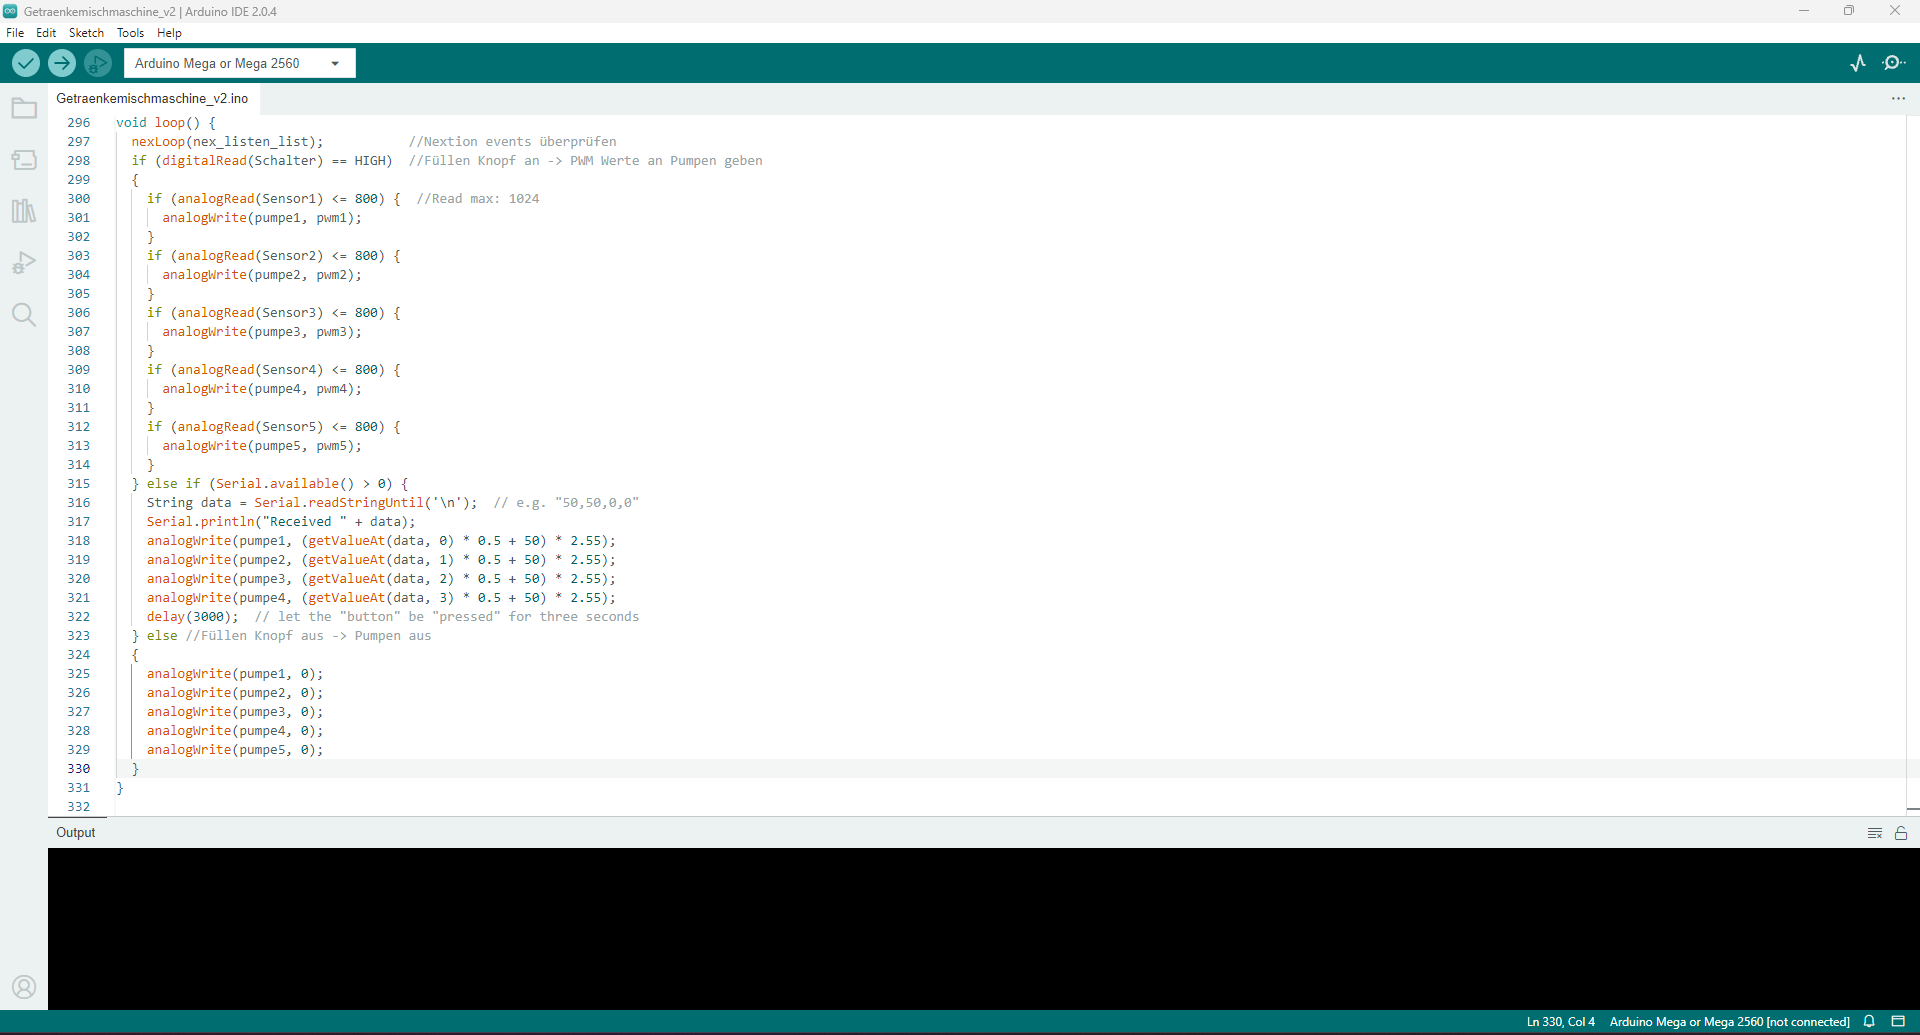
\includegraphics[width=\textwidth]{./img/Bilder_Stand_der_Technik/arduino_ide.png}}
    \caption{Arduino-IDE}
    \label{img:arduino_ide}
\end{figure}
\noindent
Ein Arduino-Mikrocontroller wird programmiert, indem das Programm in der Arduino-IDE und -Sprache geschrieben wird. Anschließend kann der Mikrocontroller über die USB-Schnittstelle an den Computer angeschlossen und der Quellcode durch Knopfdruck in der Entwicklungsumgebung an den Mikrocontroller gesendet werden, der sofort mit der Ausführung des Programms beginnt. Die meisten Mikrocontroller unterstützen kein Debugging um den Entwickler bei der Programmierung und Fehlersuche zu unterstützen. Manche Modelle verfügen jedoch über einen in Hardware implementierten Debugger zu diesem Zweck, der ebenfalls über die Entwicklungsumgebung verwendet werden kann.\\\\
Die Arduino-Programmiersprache ist angelehnt an \textit{Wiring} \cite{wiring} und kann durch eigene C++-Bibliotheken erweitert werden. Die Programmstruktur ist fest vorgegeben. Jedes Arduino-Programm besteht aus einer \textit{setup} und einer \textit{loop} Funktion. Die \textit{setup} Funktion wird exakt einmal zu Beginn des Programms aufgerufen, also wenn der Arduino mit Strom versorgt wird. Die \textit{loop} Funktion stellt die Hauptbefehlsschleife dar und enthält den Code, der den Großteil der Programmlogik enthält. Sie wird in einer Dauerschleife immer wieder neu aufgerufen. Listing \ref{arduino_example} stellt den Aufbau eines Arduino-Programms dar.\\
\lstinputlisting[language=c++, style=algoBericht, label={arduino_example}, basicstyle=\tiny\sffamily, captionpos=b, caption={Aufbau eines Arduino-Programms}]{./Listings/example.ino}
Die Arduino-Sprache stellt einige Sprachelemente bereit, die den Umgang mit der zugrundeligenden Hardware ermöglichen und erleichtern. Mit Sprachelementen sind sowohl innerhalb des Codes zugreifbare, globale Funktionen als auch Objekte gemeint. Abgesehen von \textit{setup} und \textit{loop} sind die wichtigsten Sprachelemente \cite{arduino_language}: 
\begin{itemize}
    \item \textit{digitalRead()} und \textit{digitalWrite()}:
    \item \textit{pinMode()}:
    \item \textit{analogRead()} und \textit{analogWrite()}:
    \item \textit{delay()}:
    \item \textit{Serial}:
    \item \textit{HIGH} und \textit{LOW}:
    \item \textit{INPUT} und \textit{OUTPUT}:
\end{itemize}
\subsubsection{Elegoo Mega 2560 R3}
Bei dem \textit{Elegoo Mega 2560 R3} handelt es sich um eine Nachahmung des Arduino Mega 2560 R3. Der \textit{Elegoo Mega 2560 R3} ist der, in der Mischmaschine eingebaute, Mikrocontroller und soll im Folgenden kurz vorgestellt werden.
\subsection{Nextion}
\subsection{Raspberry Pi}
\section{Sprachverarbeitung}
Im Zuge des technologischen Fortschritts nutzen die Menschen heutzutage zunehmend Sprachassistenten für verschiedene Aufgaben. 
Einer der Hauptvorteile der Sprachsteuerung ist die Bequemlichkeit und Geschwindigkeit, mit der Aufgaben erledigt werden können, ohne dass man tippen oder mit der Maus klicken muss. 
Sprachassistenten nutzen die Verarbeitung natürlicher Sprache, um Befehle zu erkennen und zu verstehen, die der Nutzer laut ausspricht.\\\\
Die Verarbeitung natürlicher Sprache - \ac{NLP} - ist eine wichtige Technologie, die es Computern ermöglicht, die von Menschen verwendete natürliche Sprache zu verstehen. 
Diese Technologie ermöglicht es Computern, menschliche Sprache zu erkennen und zu interpretieren und Text und Sprache in natürlicher Sprache zu erzeugen. 
Im Bereich der Sprachsteuerung spielt \ac{NLP} eine Schlüsselrolle bei der Erkennung von Sprache und dem Verstehen von Befehlen, die der Benutzer laut ausspricht. 
Es wird verwendet, um die Sprache des Benutzers in Text umzuwandeln, den ein Computer verstehen und verarbeiten kann.
Um dies zu erreichen, verwendet \ac{NLP} eine Vielzahl von Techniken und Technologien, darunter maschinelles Lernen, Tonanalyse, syntaktische Analyse und mehr. \cite{jurafsky_speech_2009}\\\\
Im Rahmen dieses Projekts erfordert die Implementierung der Sprachsteuerung einer Getränkemischmaschine die Verarbeitung natürlicher Sprache, damit die Maschine Befehle verstehen kann, die der Benutzer laut ausspricht. 
Dieses Projekt ähnelt einem Chatbot, bei dem der Benutzer eine Frage stellen oder einen Befehl geben kann und der Chatbot führt die entsprechende Aktion aus. 
Die Verarbeitung natürlicher Sprache ist für die Entwicklung eines solchen Sprachsteuerungssystems unerlässlich und ermöglicht es der Maschine, Befehle in natürlicher Sprache zu verstehen und auszuführen.\\\\
Eine der wichtigsten Komponenten der Verarbeitung natürlicher Sprache ist die Spracherkennung und das Syntaxanalyseverfahren. 
Bei der Spracherkennung kommen Deep-Learning-Techniken zum Einsatz, die es einem Computer ermöglichen, Sprachlaute zu erkennen und in Text zu übersetzen. 
Anschließend wird das Syntaxanalyseverfahren verwendet, um die Satzstruktur zu bestimmen und Schlüsselwörter und -sätze hervorzuheben, die zur Bestimmung des Benutzerbefehls verwendet werden können.
Auch die Tonwertanalyse ist ein wichtiger Bestandteil der Verarbeitung natürlicher Sprache. 
Mit Hilfe der Tonalitätsanalyse lässt sich die emotionale Färbung des Textes bestimmen, was für die Ermittlung der Absicht des Nutzers nützlich sein kann. 
Da die Tonwertanalyse im Rahmen dieser Arbeit nicht relevant ist, wird sie nicht weiter erörtert.\\\\
Darüber hinaus werden grammatik- und regelbasierte Technologien zur Verarbeitung natürlicher Sprache eingesetzt. 
Diese Technologien werden eingesetzt, um die korrekte Struktur des Benutzerbefehls zu bestimmen und Schlüsselwörter hervorzuheben, die zur Durchführung von Aktionen verwendet werden können. 
Außerdem werden Techniken des maschinellen Lernens eingesetzt, damit der Computer aus früheren Befehlen und Aktionen \glqq{}lernen\grqq{} kann, was die Genauigkeit der Erkennung von Benutzerbefehlen verbessert.\\\\
Daher ist der Einsatz von Technologien zur Verarbeitung natürlicher Sprache für das Projekt der Sprachmischmaschine unerlässlich. 
Die Verarbeitung natürlicher Sprache wird es der Maschine ermöglichen, die Befehle zu verstehen und zu verarbeiten, die der Benutzer laut ausspricht und die entsprechenden Aktionen durchzuführen.
\subsection{Verarbeitung natürlicher Sprache}
Die Verarbeitung natürlicher Sprache ist ein Forschungsbereich der Informatik und der \ac{KI}, der sich mit der Verarbeitung natürlicher Sprache befasst. 
Bei der Verarbeitung geht es in der Regel darum, natürliche Sprache in Daten zu übersetzen, die ein Computer nutzen kann, um Informationen über die Welt um ihn herum zu erhalten.\\\\
Die \ac{NLP}-Pipeline, die zur Erstellung eines Dialogsystems erforderlich ist, erfordert vier Arten der Verarbeitung sowie eine Datenbank zur Speicherung vergangener Äußerungen und Antworten. 
Jeder dieser Schritte kann einen oder mehrere Verarbeitungsalgorithmen enthalten, die parallel oder sequentiell arbeiten \cite{lane_natural_2019}:
\begin{itemize}
    \item Syntaktische Zergliederung - Extraktion von Merkmalen (strukturierte numerische Daten) aus natürlichem Text.
    \item Analyse - Erstellen und Kombinieren von Items, um Indikatoren für den Ton, die grammatikalische Korrektheit und die Semantik des Textes zu erhalten.
    \item Generierung - Generierung möglicher Antworten mit Hilfe von Mustern, Suchwerkzeugen oder Sprachmodellen.
    \item Ausführung - bereitet Aussagen vor, die auf der Geschichte und dem Zweck des Gesprächs basieren und wählt eine Folgeantwort.
\end{itemize}
\begin{figure}[H]
    \centering
    \fbox{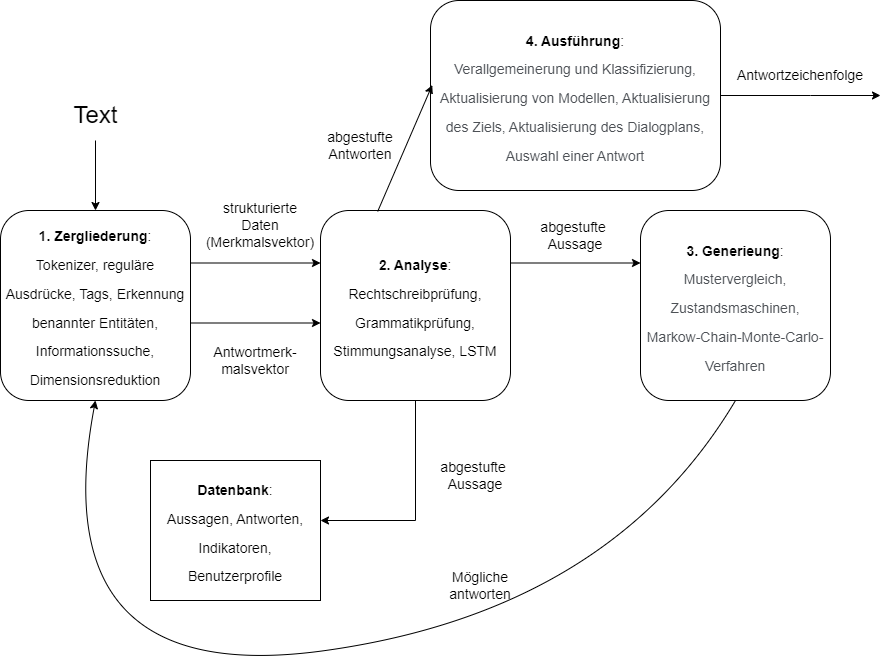
\includegraphics[width=0.8\textwidth]{Bilder_Stand_der_Technik/Chat-Bot-Pipeline.png}}
    \caption{Rekurrente Chat-Bot-Pipeline}
    \label{figure:Chat-Bot-Pipeline}
\end{figure}
\noindent
Die meisten Chatbots enthalten Elemente aus allen fünf Teilsystemen (die vier Verarbeitungsstufen sowie die Datenbank). 
Viele Anwendungen erfordern jedoch nur einfache Algorithmen, um viele dieser Schritte auszuführen. 
Ein Chatbot oder virtueller Assistent für Verbraucher wie Alexa oder Allo ist in der Regel so konzipiert, dass er äußerst sachkundig und leistungsfähig ist. 
Die Logik, die zur Beantwortung von Anfragen verwendet wird, ist jedoch oft oberflächlich und besteht aus einer Reihe von Codephrasen, die mit einer einzigen if-then-Entscheidungsverzweigung zur gleichen Antwort führen. 
Alexa (und die zugrundeliegende Lex-Engine) verhält sich wie ein einschichtiger, flacher Baum von Operatoren (if, elif, elif...). 
Andererseits stützt sich die Google Translate-Pipeline (oder jedes ähnliche maschinelle Übersetzungssystem) auf eine mehrstufige Hierarchie von Merkmalsextraktoren, Entscheidungsbäumen und Wissensgraphen, die Fragmente von Wissen über die Welt miteinander verbinden.\\\\
Alle \ac{NLP}-Merkmale müssen gut funktionieren, damit das Dialogsystem richtig funktioniert:
\begin{itemize}
    \item Merkmalsextraktion (normalerweise zur Erstellung eines Vektorraummodells).
    \item Informationssuche zur Beantwortung von Sachfragen.
    \item Semantische Suche, um Informationen aus zuvor aufgezeichneten natürlichsprachlichen Texten oder Dialogen zu assimilieren.
    \item Generierung von natürlicher Sprache, um neue sinnvolle Aussagen zu verfassen.
\end{itemize}
\subsection{Tokenisierung von Wörtern}
Eine der wichtigsten Aufgaben der Verarbeitung natürlicher Sprache ist die Tokenisierung, d. h. die Zerlegung von Text in einzelne Wörter oder Phrasen, die so genannten Token. 
Dieser Prozess ist ein wichtiger Bestandteil der Verarbeitung natürlicher Sprache, da er es Programmen und Algorithmen ermöglicht, Texte anhand ihrer Bestandteile zu verstehen und zu analysieren. 
Die Tokenisierung ist für die Verarbeitung natürlicher Sprache von entscheidender Bedeutung, da sie es Programmen ermöglicht, Schlüsselwörter, Phrasen und semantische Einheiten in einem Text hervorzuheben. 
Die Tokenisierung kann auch dazu verwendet werden, nicht benötigte Textelemente wie Satzzeichen, Leerzeichen und andere Zeichen, die keine Bedeutung haben, zu entfernen. 
Dadurch können Programme und Algorithmen effizienter und genauer arbeiten und die Wahrscheinlichkeit von Fehlern und falscher Textverarbeitung verringern.\\\\
Im \ac{NLP} ist die Tokenisierung eine besondere Art der Segmentierung von Dokumenten. 
Bei der Segmentierung wird der Text in kleinere Abschnitte (Segmente) mit engerem Informationsgehalt unterteilt. 
Die Segmentierung kann die Aufteilung eines Dokuments in Absätze, in Sätze, in Phrasen und in Token (Wörter) sowie Satzzeichen umfassen. 
Ein Tokenizer kann mit einem Scanner im Kompilierungsprozess verglichen werden. 
Token sind in diesem Fall die Endpunkte von kontextfreien Grammatiken - \ac{CFG} - zur Analyse von Programmiersprachen-Terminalen.\\\\
Die Tokenisierung ist der erste Schritt in der \ac{NLP}-Pipeline und kann daher den Rest der Pipeline stark beeinflussen. 
Der Tokenizer zerlegt unstrukturierte Daten, d. h. natürlichsprachliche Texte, in Informationseinheiten, die als einzelne Elemente gezählt werden können. 
Die so gezählte Anzahl von Token-Vorkommen in einem Dokument kann direkt als Vektor verwendet werden, der dieses Dokument repräsentiert. 
Ein solcher Ansatz ermöglicht es, aus einer unstrukturierten Zeichenfolge (einem Textdokument) unmittelbar eine für das maschinelle Lernen geeignete numerische Datenstruktur zu gewinnen. 
Diese Werte können den Computer direkt dazu veranlassen, nützliche Aktionen durchzuführen und Reaktionen zu erzeugen.\\\\
Die einfachste Art, einen Satz zu tokenisieren, ist die Verwendung von Leerzeichen als Worttrenner in Zeichenketten. 
Dies ist jedoch nicht optimal, denn wenn ein Satz z. B. ein Satzzeichen enthält, wird es von einem der Tokenisierer erfasst. 
Optimierte Tokenizer sind in mehreren Python-Bibliotheken implementiert, die jeweils ihre eigenen Vor- und Nachteile haben: spaCy, Stanford CoreNLP und \ac{NLTK}. 
\ac{NLTK} und StanfordCoreNLP sind die am längsten bestehenden und am häufigsten verwendeten Bibliotheken zum Vergleich von \ac{NLP}-Algorithmen in wissenschaftlichen Artikeln. 
Obwohl die StanfordCoreNLP-Bibliothek eine Python-\ac{API} hat, basiert sie auf dem Java 8 CoreNLP-Anwendungsteil, der separat installiert und konfiguriert werden muss. 
Daher wurde in dieser Arbeit der \ac{NLTK}-Tokenizer verwendet.\\\\
Ein wichtiges Konzept im Tokenisierungsprozess sind N-Gramme. 
Ein N-Gramm ist eine Sequenz mit bis zu n Elementen, die aus einer Sequenz dieser Elemente, in der Regel einer Zeichenkette, extrahiert wurden. 
Im Allgemeinen können die Elemente eines N-Gramms Buchstaben, Silben, Wörter oder sogar Symbole sein. 
N-Gramme sind notwendig, weil bei der Konvertierung einer Menge von Wörtern in einen Vektor eine Folge von Token einen Großteil der Bedeutung verliert, die in der Reihenfolge dieser Wörter verkapselt ist. 
Wenn das Token-Konzept auf Mehrwort-Token, N-Gramme, ausgedehnt wird, kann die \ac{NLP}-Pipeline einen erheblichen Teil der Bedeutung, die in der Wortfolge dieser Äußerungen enthalten ist, beibehalten. 
So bleibt beispielsweise das Wort \glqq{}kein\grqq{}, das die Bedeutung umkehrt, neben den benachbarten Wörtern stehen, wo es hingehört. 
Ohne N-Gramm-Tokenisierung würde ein solches Wort an verschiedenen Positionen herumhängen und seine Bedeutung würde mit dem gesamten Satz oder Dokument assoziiert werden, anstatt mit benachbarten Wörtern. 
Das Bigramm \glqq{}war nicht\grqq{} behält viel mehr Bedeutung der einzelnen Wörter \glqq{}war\grqq{} und \glqq{}nicht\grqq{} als die entsprechenden Singlegramme im Multigrammvektor. 
Durch die Verknüpfung eines Wortes mit seinen Nachbarn in einem Förderband kann ein Teil seines Kontexts erhalten bleiben. 
N-Gramme sind also ein Instrument zur Speicherung von Kontextinformationen, während die Daten die Pipeline durchlaufen.\\\\
Die Größe des Vokabulars spielt eine wichtige Rolle für die Leistung der \ac{NLP}-Pipeline. 
Die Größe des Wörterbuchs bestimmt die Größe der Trainingsstichprobe, die benötigt wird, um eine Überanpassung an ein bestimmtes Wort oder eine bestimmte Phrase zu vermeiden und die Größe der Trainingsmenge bestimmt die Kosten der Verarbeitung. 
Eine Technik zur Verringerung der Größe des Wörterbuchs besteht darin, Token, die ähnliche Dinge bedeuten, in einer einzigen normalisierten Form zusammenzufassen. 
Eine solche Technik reduziert die Anzahl der gespeicherten Token und verbessert die Verbindungen zwischen den Bedeutungen von Phrasen mit unterschiedlicher \glqq{}Schreibweise\grqq{} der Tokens und verringert die Wahrscheinlichkeit des Überlernens. 
Eine der Normalisierungsmöglichkeiten ist die Groß- und Kleinschreibung - die Kombination mehrerer Schreibweisen eines Wortes, die sich nur in der Groß- und Kleinschreibung unterscheiden. 
In diesem Fall wird die Groß-/Kleinschreibung ignoriert und zwei identische Wörter, von denen eines groß und das andere klein geschrieben wird, werden als dasselbe Token behandelt.\\\\
Ein weiterer wichtiger Schritt bei der Tokenisierung von Texten ist die Entfernung von Stoppwörtern, um den Umfang des Wörterbuchs zu verringern. 
Stoppwörter sind in jeder Sprache gebräuchliche Wörter, die sehr häufig vorkommen, aber sehr viel weniger aussagekräftige Informationen über die Bedeutung eines Satzes enthalten (z. B. a, an, the, this, of, on im Englischen oder der, die, das, diese im Deutschen). 
Stoppwörter können jedoch nützliche Informationen enthalten, so dass man sie nicht immer verwerfen sollte. 
Das \ac{NLTK}-Paket für Python enthält derzeit die umfassendste Liste kanonischer Stoppwörter in verschiedenen Sprachen.\\\\
Eine weitere gängige Methode der Normalisierung ist die Beseitigung kleiner semantischer Unterschiede im Zusammenhang mit Pluralendungen und Possessivendungen von Wörtern oder sogar unterschiedlichen Verbformen. 
Diese Methode der Normalisierung, bei der ein gemeinsamer Wortstamm für verschiedene Wortformen gefunden wird, wird als Stemming bezeichnet. 
Der gemeinsame Wortstamm von \glqq{}Gehäuse\grqq{} und \glqq{}Haus\grqq{} ist zum Beispiel \glqq{}Haus\grqq{}.
 Beim Stemming werden Suffixe von Wörtern entfernt, um Wörter mit ähnlicher Bedeutung unter einem gemeinsamen Stamm zu gruppieren. 
 Der Wortstamm muss nicht unbedingt ein gültiges Wort sein, sondern kann auch nur ein Token oder eine Bezeichnung sein, das mehrere mögliche Schreibweisen repräsentiert. 
 Einer der Hauptvorteile des Stemming besteht darin, die Anzahl der Wörter zu verringern, deren Bedeutung das Sprachmodell im Auge behalten muss. 
 Durch diese Methode wird die Größe des Wörterbuchs reduziert, wodurch der Verlust nützlicher Informationen und Bedeutungen so weit wie möglich begrenzt wird. 
 Das Stemming spielt eine wichtige Rolle bei der Suche nach Schlüsselwörtern oder Informationen. 
Zwei der bekanntesten Algorithmen sind Porter's Stemmer und Snowball.\\\\
Mit Informationen über die Beziehungen zwischen den Bedeutungen verschiedener Wörter ist es möglich, mehrere Wörter miteinander zu verknüpfen, auch wenn ihre Schreibweise sehr unterschiedlich ist. 
Eine solche erweiterte Normalisierung eines Wortes auf seine semantische Wurzel - ein Lemma - wird Lemmatisierung genannt. 
Die Lemmatisierung ist potenziell eine viel genauere Art der Normalisierung als das Stemming oder die Groß- und Kleinschreibung, da sie die Bedeutung des Wortes berücksichtigt. 
Der Lemmatisierer verwendet eine Wissensbasis von Synonymen und Wortendungen, um nur eng verwandte Wörter zu einem Token zu kombinieren. 
In Python kann die Lemmatisierung mit dem \ac{NLTK}-Paket implementiert werden, das den \textit{WordNetLemmatizer} enthält.\\\\
Wie bereits gezeigt wurde, ist die Tokenisierung der Prozess der Zerlegung von Text in einzelne Wörter oder Token. 
Für viele Anwendungen der Verarbeitung natürlicher Sprache ist jedoch nicht nur wichtig, welche Wörter im Text enthalten sind, sondern man muss auch in der Lage sein, diese Wörter als Zahlen darzustellen. 
Dadurch wird es möglich, maschinelles Lernen und andere Algorithmen, die mit Zahlen arbeiten, zur Textverarbeitung einzusetzen. 
Bei der Verarbeitung natürlicher Sprache wird dazu die Wortvektorisierung verwendet.
\subsection{Vektorisierung von Wörtern}
Die Vektorisierung hilft dabei, eine numerische Darstellung zu finden, die die Bedeutung oder den Informationsgehalt der dargestellten Wörter widerspiegelt. 
Es gibt drei Möglichkeiten, Wörter und ihre Bedeutungen darzustellen:
\begin{itemize}
    \item Multisets von Wörtern - Vektoren von Zahlen oder Häufigkeiten von Wörtern. 
    \item Multisets von N-Grammen - Vektoren von Mengen von Wortpaaren (Bigramme), Worttripeln (Trigramme), usw.
    \item \ac{TF}-\ac{IDF}-Vektoren sind Indikatoren für Wörter, die deren Bedeutung am Besten darstellen.
\end{itemize}
Jede dieser Methoden kann entweder allein oder als Teil einer \ac{NLP}-Pipeline angewendet werden. 
Alle beschriebenen Modelle sind statistisch in dem Sinne, dass sie auf Worthäufigkeiten beruhen.
\subsubsection{Multisets von Wörtern}
\ac{BOW}-Vektoren sind Vektoren, die Textdokumente als Wort-Multisets (Bags) darstellen, wobei ein Multiset eine Sammlung von Elementen ist, in der jedes Element mehr als einmal wiederholt werden kann. 
Ein Wort-Bag ist eine Darstellung von Text, die das Vorkommen von Wörtern in einem Dokument beschreibt. 
Sie beinhaltet zwei Dinge:
\begin{enumerate}
    \item Ein Wörterbuch mit bekannten Wörtern.
    \item Ein Maß für das Vorhandensein von bekannten Wörtern.
\end{enumerate}
Dies wird als \glqq{}Word-Bag\grqq{} bezeichnet, weil alle Informationen über die Reihenfolge oder Struktur der Wörter im Dokument verworfen werden. 
Das Modell interessiert sich nur dafür, ob bekannte Wörter im Dokument vorkommen, nicht aber, wo im Dokument. 
Bei diesem Ansatz wird das Histogramm der Wörter im Text betrachtet, d. h. wir betrachten jedes Wort als ein Merkmal \cite{goldberg_neural_2017}.\\\\
Ein Ansatz zur Vektorisierung einer Vielzahl von Wörtern besteht darin, für jedes Wort einen Einheitsvektor zu erstellen und diese Vektoren dann zu einem einzigen Vektor zu kombinieren. 
Ein unitärer Vektor für ein Wort ist ein Vektor, dessen Länge der Dimension des Raumes entspricht und alle seine Komponenten sind Null, mit Ausnahme einer Komponente, die der Position des Wortes im Wörterbuch entspricht. Unitäre Vektoren sind extrem spärlich. 
Enthält das Wörterbuch beispielsweise 1000 Wörter, dann hat jeder unitäre Vektor eine Dimension von 1000 und die Komponente, die der Position des Wortes im Wörterbuch entspricht, ist gleich eins.
Zum Beispiel sieht der unitäre Vektor für den Satz \glqq Mojito ist ein leckerer Cocktail\grqq{} (nach dem Tokenisierungsprozess) so aus:
\begin{figure}[H]
    \centering
    \fbox{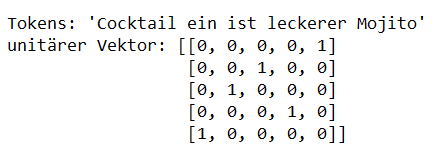
\includegraphics[width=0.6\textwidth]{Bilder_Stand_der_Technik/unitaerer_vektor.png}}
    \caption{\label{figure:Unitaere_Vektoe}Unitärer Vektor}
\end{figure}
\noindent
Eine der Eigenschaften der vektoriellen Darstellung von Wörtern und der tabellarischen Darstellung von Dokumenten ist, dass keine ursprünglichen Informationen verloren gehen. 
Das Originaldokument kann aus dieser einheitlichen Vektortabelle rekonstruiert werden. 
Daher werden solche unitären Vektoren in neuronalen Netzen, bei der \ac{seq2seq}-Modellierung und bei der Erstellung von Sprachmodellen verwendet. 
Unitäre Vektoren eignen sich hervorragend für alle \ac{NLP}-Modelle oder -Pipelines, bei denen die Bedeutung des Ausgangstextes vollständig erhalten bleiben muss.
Die Erstellung von unitären Vektoren für jedes Wort kann mit verschiedenen Bibliotheken in Python erfolgen. 
Zum Beispiel kann die NumPy-Bibliothek verwendet werden, um unitäre Vektoren zu erstellen.\\\\
Diese Vektordarstellung hat jedoch ihre Nachteile. 
Bei Dokumenten, die eine große Anzahl von Wörtern enthalten, wäre die Größe des unitären Vektorwörterbuchs enorm und würde enorme Ressourcen zur Verarbeitung erfordern. 
Außerdem macht es keinen Sinn, so viele Nullen zu speichern. 
Um mit dem Wörterbuch arbeiten zu können, ohne viel Zeit für die Verarbeitung zu verschwenden, ist es notwendig, das Wörterbuch zu verkleinern. 
Dazu ist es notwendig, auf die Möglichkeit der Rekonstuierung des Originaldokuments zu verzichten, d.h. sich die Wortfolge aller Dokumente zu merken. 
Es ist notwendig, den größten Teil der Informationen zu erfassen, nicht das gesamte Dokument. Dafür sind Multiset-Vektoren hilfreich.\\\\
Um einen Vektor für ein Multiset von Wörtern zu erstellen, müssen für jedes Wort der Mehrmenge ein Einheitsvektor erstellt und diese Vektoren dann zu einem einzigen Vektor kombiniert werden. 
Vektoren können nach verschiedenen Regeln kombiniert werden, z. B. durch Addition, Multiplikation, Verkettung oder andere Operationen. 
Wenn alle diese unitären Vektoren zusammengezählt werden, wird ein Vektor der Worthäufigkeit erhalten. 
Er spiegelt die Häufigkeit des Vorkommens von Wörtern wider, nicht die Reihenfolge, in der sie auftreten. 
Dieser Vektor kann verwendet werden, um ein ganzes Dokument oder einen Satz als einen einzigen Vektor von nicht sehr großer Länge darzustellen. 
Seine Länge entspricht der Länge des Wörterbuchs (der Anzahl der verfolgten eindeutigen Token). 
Außerdem kann bei einer einfachen Schlüsselwortsuche ein binärer Multiset-Vektor durch eine logische OR-Operation aus unitären Vektoren gewonnen werden.\\\\
Die Anzahl der Vorkommen eines Wortes in einem bestimmten Dokument wird als Termfrequenz (\ac{TF}) bezeichnet. 
Je häufiger ein Wort in einem Dokument vorkommt, desto wahrscheinlicher ist es, dass das Dokument von diesem Thema handelt. 
Anstelle von reinen Wortzählungen können auch normalisierte Termhäufigkeiten zur Beschreibung von Dokumenten aus einem Korpus verwendet werden. 
Unter normalisierten Dokumenthäufigkeiten versteht man die Anzahl der Wörter im Verhältnis zur Länge des Dokuments. 
Die Normalisierung ist sehr nützlich, um die Bedeutung eines Dokuments zu ermitteln, da reine Häufigkeiten nicht immer die tatsächliche Situation widerspiegeln. 
Wenn beispielsweise das Wort \glqq Cocktail\grqq{} 15 Mal in Dokument \textnumero 1 und 400 Mal in Dokument \textnumero 2 vorkommt, kann man daraus schließen, dass es in Dokument Nummer zwei eher um Cocktails geht.
Vielleicht handelt es sich aber bei Dokument \textnumero 1 um ein Rezept für die Zubereitung von Mai Tais mit 100 Wörtern, während Dokument \textnumero 2 ein Roman mit 500.000 Wörtern ist, in dem die Figuren gelegentlich Cocktails trinken. 
Die Häufigkeit des Wortes \glqq Cocktail\grqq{} in Dokument \textnumero 1 beträgt also 0,15 und 0,0008 in Dokument \textnumero 2, was die tatsächliche Bedeutung des Begriffs \glqq Cocktail\grqq{} in diesen Dokumenten viel besser widerspiegelt:
\begin{figure}[H]
    \centering
    \fbox{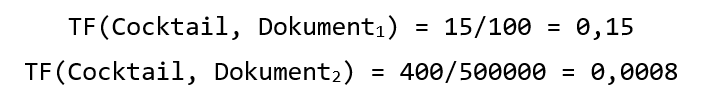
\includegraphics[width=0.8\textwidth]{Bilder_Stand_der_Technik/norm_vektoren.png}}
    \caption{\label{figure:Norm_Vektoren}Normalisierte \ac{TF}-Vektoren}
\end{figure}
\noindent
Ebenso ist es möglich, diesen Wert für jedes Wort zu berechnen und die relative Bedeutung dieses Begriffs für jedes Dokument zu ermitteln, woraus sich die Bedeutung jedes Dokuments ableiten lässt. 
Um die Anzahl der Vorkommen von Wörtern zu ermitteln, kann das Objekt \textit{collections.Counter} in Python verwendet und anschließend eine Normalisierung durchgeführt werden:
\begin{figure}[H]
    \centering
    \fbox{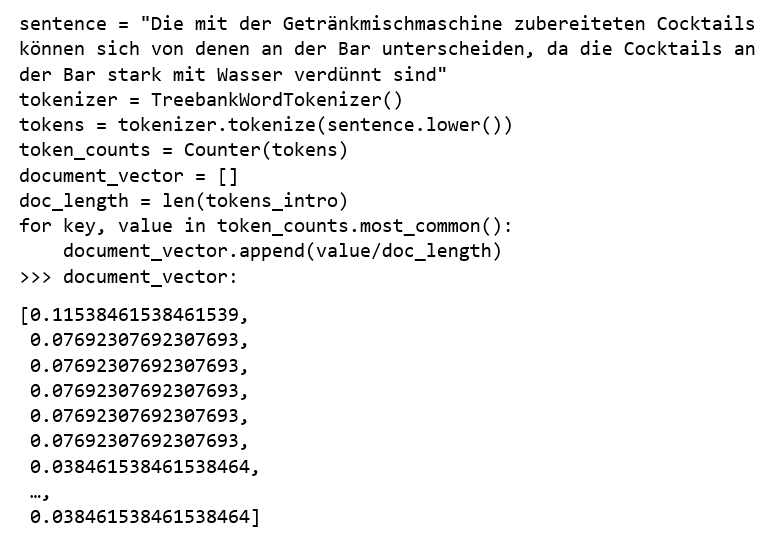
\includegraphics[width=0.8\textwidth]{Bilder_Stand_der_Technik/norm_vek_py.png}}
    \caption{\label{figure:Norm_Vektoren_Python}Normalisierte \ac{TF}-Vektoren mit Python}
\end{figure}
\noindent
Wenn mehr als ein Dokument bearbeitet wird, wird für jedes Dokument ein eigener Häufigkeitsvektor erstellt, der jedoch absolut alle Begriffe aus allen Dokumenten (alle Wörter aus dem Wörterbuch) enthält, auch wenn einige der Wörter nicht in allen Dokumenten vorkommen. 
In diesem Fall werden die Vektoren an diesen Stellen Nullwerte enthalten.\\\\
Das ultimative Ziel der Textvektorisierung besteht darin, natürliche Sprache in ein Format zu übersetzen, das der Computer verstehen kann. 
Eine Möglichkeit, dies zu erreichen, ist die Verwendung von Vektorräumen. 
Vektorräume sind mathematische Objekte, in denen jedes Element durch einen Vektor dargestellt wird und verschiedene Operationen mit Vektoren ermöglichen es uns, nützliche Merkmale zu extrahieren. 
So wird ein Vektor mit zwei Werten in einem zweidimensionalen Vektorraum verortet, ein Vektor mit drei Werten in einem dreidimensionalen Vektorraum und so weiter. 
Beispielsweise ist der Vektorraum von Dokumenten, die nur aus den Wörtern \glqq Cocktail\grqq{} und \glqq Maschine\grqq{} bestehen, zweidimensional und die Vektoren der enthaltenen Dokumente können wie folgt dargestellt werden:
\begin{figure}[H]
    \centering
    \fbox{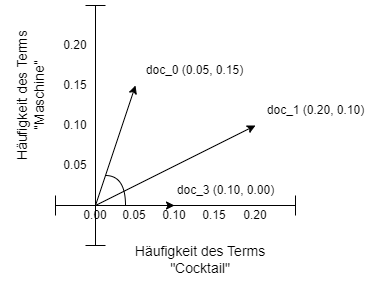
\includegraphics[width=0.6\textwidth]{Bilder_Stand_der_Technik/vraum.png}}
    \caption{\label{figure:Vraum}Zweidimensionale Vektoren von Termhäufigkeiten}
\end{figure}
\noindent
Für einen Vektorraum von Dokumenten in einer natürlichen Sprache ist die Dimensionalität des Vektorraums gleich der Anzahl der verschiedenen Wörter im gesamten Korpus. 
Jedes Dokument in einem K-dimensionalen Vektorraum kann durch einen K-dimensionalen Vektor beschrieben werden. 
Wenn es Vektorrepräsentationen für alle Dokumente im gleichen Raum gibt, dann ist es möglich, sie zu vergleichen. 
Der euklidische Abstand zwischen Vektoren kann gemessen werden, indem sie subtrahiert werden und die Länge des Abstands zwischen ihnen berechnet wird, den sogenannten Abstand im Sinne der L2-Norm (L2-Metrik). 
Dies ist der Abstand auf einer geraden Linie von dem Ort, der durch die Spitze (Scheitelpunkt) des einen Vektors gegeben ist, zu dem Ort, der der Spitze des anderen Vektors entspricht.
\begin{figure}[H]
    \centering
    \fbox{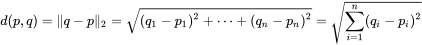
\includegraphics[width=0.6\textwidth]{Bilder_Stand_der_Technik/l2.png}}
    \caption{\label{figure:euklidische_Norm}Euklidische Norm}
\end{figure}
\noindent
Der Ochiai-Koeffizient (Kosinuskoeffizient) ist ein Maß für die Ähnlichkeit zwischen zwei Multisets. 
Der Ochiai-Koeffizient kann verwendet werden, um den Grad der Ähnlichkeit zwischen zwei Dokumenten auf der Grundlage ihrer Wort-Multisets zu bestimmen. 
Er ist einfach der Kosinus des Winkels zwischen zwei Vektoren (Theta).
\begin{figure}[H]
    \centering
    \fbox{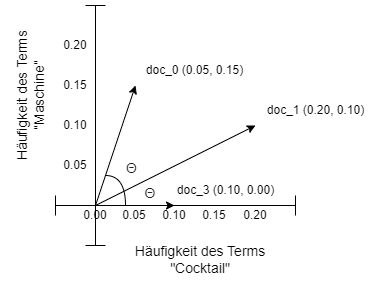
\includegraphics[width=0.6\textwidth]{Bilder_Stand_der_Technik/vraum_theta.png}}
    \caption{\label{figure:Vraum_Theta}Zweidimensionale Theta}
\end{figure}
\noindent
Er kann mithilfe des euklidischen Skalarprodukts nach folgender Formel berechnet werden:
\begin{figure}[H]
    \centering
    \fbox{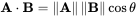
\includegraphics[width=0.2\textwidth]{Bilder_Stand_der_Technik/euk_dot_prod.png}}
    \caption{\label{figure:Euklidisches_Skalarprodukt}Euklidisches Skalarprodukt}
\end{figure}
\noindent
\begin{figure}[H]
    \centering
    \fbox{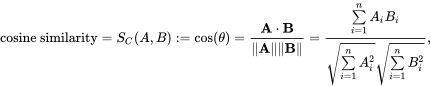
\includegraphics[width=0.6\textwidth]{Bilder_Stand_der_Technik/ochiai_koef.png}}
    \caption{\label{figure:Ochiai_Koeffizient}Ochiai-Koeffizient}
\end{figure}
\noindent
Das Skalarprodukt zweier Vektoren kann also berechnet werden, indem die Elemente der Vektoren paarweise multipliziert und dann die Ergebnisse addiert werden. 
Anschließend wird das Ergebnis durch die Norm jedes Vektors dividiert. 
Die Norm eines Vektors ist gleich dem euklidischen Abstand zwischen seinem Kopf und seinem Ende - der Quadratwurzel aus der Summe der Quadrate seiner Elemente. 
Dieses normierte Skalarprodukt liegt wie der Kosinuswert zwischen -1 und 1. 
Es ist auch der Kosinus des Winkels zwischen den beiden Vektoren. 
Dieser Wert ist gleich dem Anteil des längeren Vektors, der von der senkrecht dazu stehenden Projektion des kürzeren Vektors abgedeckt wird. 
Daraus ist ersichtlich, wie weit unsere beiden Vektoren in dieselbe Richtung zeigen.\\\\
Ein offensichtlicher Vorteil ist, dass der vom Ochiai-Koeffizienten angenommene Wertebereich (von -1 bis +1) für die meisten Aufgaben des maschinellen Lernens geeignet ist. 
Ein Kosinuskoeffizient von 1 spiegelt identische normalisierte Vektoren wider, die über alle Dimensionen hinweg in eine ähnliche Richtung zeigen. 
Die Längen dieser Vektoren können unterschiedlich sein, aber sie zeigen in dieselbe Richtung. 
Je näher der Kosinuskoeffizient bei 1 liegt, desto kleiner ist der Winkel zwischen den Vektoren. 
Im \ac{NLP} enthalten Dokumente, deren Kosinuskoeffizient der Vektoren nahe bei 1 liegt, ähnliche Wörter im gleichen Verhältnis. 
Daher ist es wahrscheinlicher, dass es sich bei Dokumenten, deren Vektoren nahe beieinander liegen, um dieselbe Sache handelt. 
Wenn der Kosinuskoeffizient 0 ist, haben die Vektoren keine gemeinsamen Komponenten. 
Sie stehen in allen Dimensionen in einem 90°-Winkel zueinander. 
Bei \ac{TF}-\ac{NLP}-Vektoren tritt diese Situation nur ein, wenn die beiden Dokumente keine gemeinsamen Wörter haben. 
Da sie völlig unterschiedliche Wörter verwenden, sprechen sie von völlig unterschiedlichen Dingen. 
Das bedeutet nicht unbedingt, dass die Bedeutung oder das Thema unterschiedlich ist, sondern nur, dass sie unterschiedliche Wörter verwenden. 
Bei einem Wert des Kosinuskoeffizient von -1 sind die Vektoren völlig entgegengesetzt. 
Sie zeigen in entgegengesetzte Richtungen. 
Bei einfachen Vektoren der Termhäufigkeiten ist dies jedoch nicht möglich, da Vektoren der Termhäufigkeiten nicht negativ sein können. 
Sie befinden sich also immer im gleichen Quadranten des Vektorraums.\\\\
Neben den Multisets von Wörtern gibt es weitere Vektorisierungsmethoden, die ebenfalls in der Verarbeitung natürlicher Sprache verwendet werden - Multisets von N-Grammen und \ac{TF-IDF}-Vektoren.
Bei Multisets von N-Grammen handelt es sich um Mengen von mehreren aufeinanderfolgenden Wörtern in einem Text. 
N-Gramme können helfen, den Kontext und die Beziehung zwischen Wörtern in einem Text zu erfassen. 
In diesem Fall wird nicht die Häufigkeit der einzelnen Begriffe im Dokument berücksichtigt, sondern die Häufigkeit des Auftretens von N-Grammen.
\ac{TF-IDF}-Vektoren sind jedoch eine noch effizientere Methode zur Vektorisierung von Text. 
Im Gegensatz zu Multisets von Wörtern und N-Grammen berücksichtigen \ac{TF-IDF}-Vektoren nicht nur die Häufigkeit von Wörtern in einem Dokument, sondern auch die Bedeutung jedes Wortes im Kontext des gesamten Textkorpus. 
So haben Wörter, die in allen Dokumenten häufig vorkommen, eine geringere Bedeutung als seltene Wörter, die dazu beitragen, ein Dokument von anderen zu unterscheiden.
\subsubsection{\ac{TF-IDF}-Vektoren}
Das \ac{TF-IDF}-Vektorkonzept ist eines der grundlegenden Werkzeuge der natürlichen Sprachverarbeitung. 
Es wird verwendet, um Textdokumente in numerische Vektoren umzuwandeln, die für Textanalyse, Dokumentenklassifikation, Empfehlungssysteme und viele andere Anwendungen verwendet werden können.\\\\
Eine der wichtigsten Fragen, die sich bei der Verarbeitung natürlicher Sprache stellen, ist die Bestimmung der Bedeutung von Wörtern in einem Text. 
Die Bedeutung von Wörtern kann anhand ihrer Häufigkeit in einem Dokument bestimmt werden. 
Einige Wörter kommen jedoch häufig in allen Dokumenten vor, so dass sie nicht allzu wichtig sein sollten. 
Andererseits können einige seltene Wörter von großer Bedeutung sein, weil sie möglicherweise nur in einem bestimmten Dokument vorkommen. 
\ac{TF-IDF}-Vektoren lösen dieses Problem, indem sie nicht nur die Häufigkeit der Wörter in einem Dokument, sondern auch ihre Bedeutung im Kontext des gesamten Textkorpus berücksichtigen. 
Für jedes Wort in einem Dokument kann sein \ac{TF-IDF}-Wert nach der folgenden Formel berechnet werden:
\begin{equation}
    TF(t, d) = \frac{Anzahl(t)}{Anzahl(d)}
    \eqlabel{eq-tf}{Wert der Worthäufigkeit im Dokument}
\end{equation}
\begin{equation}
    IDF(t, D) = \log \frac{Anzahl(D)}{Anzahl(D,\: die\: t\: beinhalten)}
    \eqlabel{eq-idf}{Wert der inversen Dokumenthäufigkeit}
\end{equation}
\begin{equation}
    TFIDF(t, d, D) = TF(t, d)\cdot IDF(t, D)
    \eqlabel{eq-tfidf}{TF-IDF-Wert}
\end{equation}
Dabei ist t ein Wort, d ein Dokument, \ac{TF}(t, d) der Wert der Worthäufigkeit im Dokument und \ac{IDF}(t, D) der Wert der inversen Dokumenthäufigkeit. 
Um einen \ac{TF-IDF}-Vektor für jedes Dokument zu erhalten, müssen die \ac{TF-IDF}-Werte für alle Wörter, die in dem Dokument vorkommen, verwendet werden. 
Dies ergibt einen Vektor, bei dem jede Komponente einem \ac{TF-IDF}-Wert für ein bestimmtes Wort im Dokument entspricht.
Beispielsweise werden die folgenden drei Dokumente betrachtet:\\
Dokument \textnumero 1 \glqq Ein Cocktail ist variationsreich und auch zuhause gut zu mixen\grqq{}\\
Dokument \textnumero 2 \glqq Der Mojito ist ein klassischer Cocktail und ein erfrischender Drink der 
immer passt\grqq{}\\
Dokument \textnumero 3 \glqq Dank unserem Rezept machen Sie diesen Cocktail selber zuhause\grqq{}\\
Zunächst müssen die Dokumente tokenisiert und unnötige Stoppwörter herausgefiltert werden, die für das Verständnis der Bedeutung der Dokumente keine große Rolle spielen. 
Nach diesem Prozess sehen die Dokumente wie folgt aus:\\
Dokument \textnumero 1 \glqq Cocktail variationsreich zuhause gut mixen\grqq{}\\
Dokument \textnumero 2 \glqq Mojito klassischer Cocktail erfrischender Drink immer passt\grqq{}\\
Dokument \textnumero 3 \glqq Dank Rezepte machen Cocktail selber zuhause\grqq{}\\
Als erstes müssen die normalisierten \ac{TF}-Vektoren jeden Terms berechnet werden:
\begin{table}[H]
    \centering
    \begin{tabular}{l|c|c|c}
        TF(t, d)          & Dokument \textnumero 1 & Dokument \textnumero 2 & Dokument \textnumero 3 \\
        \hline
        Cocktail            & 1/5 = 0.2             & 1/7 = 0.143      & 1/6 = 0.167 \\
        \hline
        variationsreich & 0.2             & 0 & 0      \\
        \hline
        zuhause                & 0.2           & 0    & 0.167 \\
        \hline
        gut                  & 0.2             & 0      & 0  \\
        \hline
        mixen            & 0.2             & 0      & 0 \\
        \hline
        Mojito & 0             & 0.143 & 0      \\
        \hline
        klassischer                & 0           & 0.143    & 0 \\
        \hline
        erfrischender                  & 0             & 0.143      & 0   \\
        \hline
        Drink            & 0             & 0.143      & 0 \\
        \hline
        immer & 0             & 0.143 & 0      \\
        \hline
        passt                & 0          & 0.143    & 0 \\
        \hline
        Dank                  & 0             & 0      & 0.167   \\
        \hline
        Rezepte            & 0             & 0      & 0.167 \\
        \hline
        machen & 0             & 0 & 0.167      \\
        \hline
        selber                & 0           & 0    & 0.167\\
    \end{tabular}
    \caption{\label{table:TF_Vektoren}\ac{TF}-Vektoren}
\end{table}
\noindent
Anschließend können die \ac{IDF}-Vektoren für jeden Term (über den gesamten Dokumentenkorpus) berechnet werden:
\begin{table}[H]
    \centering
    \begin{tabular}{l|c|c|c}
        IDF(t, D)          & Dokumentenkorpus \\
        \hline
        Cocktail            & log(3/3) = 0  \\
        \hline
        variationsreich & 0.477   \\
        \hline
        zuhause                & 0.176  \\
        \hline
        gut                  & 0.477  \\
        \hline
        mixen            & 0.477  \\
        \hline
        Mojito & 0.477  \\
        \hline
        klassischer                & 0.477  \\
        \hline
        erfrischender                  & 0.477  \\
        \hline
        Drink            & 0.477  \\
        \hline
        immer & 0.477  \\
        \hline
        passt                & 0.477  \\
        \hline
        Dank                  & 0.477 \\
        \hline
        Rezepte            & 0.477 \\
        \hline
        machen & 0.477  \\
        \hline
        selber                & 0.477  \\
    \end{tabular}
    \caption{\label{table:IDF_Vektoren}\ac{IDF}-Vektoren}
\end{table}
\noindent
Jetzt kann mit der Berechnung der \ac{TF-IDF}-Vektoren fortgefahren werden:
\begin{table}[H]
    \centering
    \begin{tabular}{l|c|c|c}
        TF-IDF(t, d, D)          & Dokument \textnumero 1 & Dokument \textnumero 2 & Dokument \textnumero 3 \\
        \hline
        Cocktail            & 0.2*0 = 0             & 0.143*0 = 0      & 0.167*0 = 0 \\
        \hline
        variationsreich & 0.0954             & 0 & 0      \\
        \hline
        zuhause                & 0.0352           & 0    & 0.03 \\
        \hline
        gut                  & 0.0954             & 0      & 0  \\
        \hline
        mixen            & 0.0954             & 0      & 0 \\
        \hline
        Mojito & 0             & 0.068 & 0      \\
        \hline
        klassischer                & 0           & 0.068    & 0 \\
        \hline
        erfrischender                  & 0             & 0.068      & 0   \\
        \hline
        Drink            & 0             & 0.068      & 0 \\
        \hline
        immer & 0             & 0.068 & 0      \\
        \hline
        passt                & 0          & 0.068    & 0 \\
        \hline
        Dank                  & 0             & 0      & 0.08   \\
        \hline
        Rezepte            & 0             & 0      & 0.08 \\
        \hline
        machen & 0             & 0 & 0.08      \\
        \hline
        selber                & 0           & 0    & 0.08\\
    \end{tabular}
    \caption{\label{table:TFIDF_Vektoren}\ac{TF-IDF}-Vektoren}
\end{table}
\noindent
Wie aus dem Beispiel ersichtlich, haben Wörter, die in allen Dokumenten vorkommen, wie z.B. \glqq Cocktail\grqq{}, in jedem Dokument den gleichen \ac{TF-IDF}-Wert, Wörter, die in mehr als einem Dokument vorkommen, wie z.B. \glqq zuhause\grqq{}, haben einen niedrigeren \ac{IDF}-Wert als seltene Wörter, wie z.B. \glqq selber\grqq{} oder \glqq{}Rezept\grqq{}, die in den Dokumenten, in denen sie vorkommen, einen hohen \ac{IDF}-Wert und damit einen hohen \ac{TF-IDF}-Wert haben. 
Diese durch die Berechnung von \ac{TF-IDF} erhaltene Zahl assoziiert also ein bestimmtes Wort oder Token mit einem bestimmten Dokument in einem bestimmten Korpus und legt dann einen numerischen Wert für die Bedeutung dieses Wortes in diesem Dokument fest, wobei sein Vorkommen im gesamten Korpus berücksichtigt wird. 
Da für jedes Wort in den Dokumenten nun \ac{TF-IDF}-Werte vorliegen, können diese zu \ac{TF-IDF}-Vektoren für jedes Dokument kombiniert werden. 
Der \ac{TF-IDF}-Vektor für jedes Dokument hat eine Dimension, die der Gesamtzahl der eindeutigen Wörter im Textkorpus entspricht. 
Jedes Element im Vektor entspricht einem bestimmten Wort und der Wert des Elements ist gleich seinem \ac{TF-IDF}-Wert für dieses Dokument. 
In diesem Beispiel sehen die \ac{TF-IDF}-Vektoren für jedes Dokument wie folgt aus:\\
Dokument \textnumero 1 [0. 0.0954 0.0352 0.0954 0.0954 0. 0. 0. 0. 0. 0. 0. 0. 0. 0.]\\
Dokument \textnumero 2 [0. 0. 0. 0. 0. 0.068 0.068 0.068 0.068 0.068 0.068 0. 0. 0. 0.]\\
Dokument \textnumero 3 [0. 0. 0.03 0. 0. 0. 0. 0. 0. 0. 0. 0.08 0.08 0.08 0.08]\\\\
Aus diesen Vektoren kann die Ähnlichkeit zwischen den Dokumenten berechnet werden, z. B. mit Hilfe des Kosinuskoeffizients. 
Je näher die Werte des Kosinuskoeffizients bei 1 liegen, desto ähnlicher sind sich die Dokumente. 
Für die maximale derzeit erreichbare Effizienz bei der semantischen Suche, der Dokumentenklassifikation, bei Dialogsystemen und den meisten anderen Anwendungen ist es daher ausreichend, nur einfache \ac{TF-IDF}-Vektoren in die Pipeline einzugeben. 
\ac{TF-IDF}-Vektoren sind die erste Stufe der Pipeline, die Grundmenge der aus dem Text extrahierten Merkmale. 
Auf der Grundlage der \ac{TF-IDF}-Vektoren können Themenvektoren berechnet werden, die für die semantische Analyse von Texten erforderlich sind.\\\\
Es gibt viele Bibliotheken, um die \ac{TF-IDF}-Vektorisierung in Python zu implementieren. 
Einige der beliebtesten Bibliotheken sind Scikit-Learn, Gensim, \ac{NLTK} und SpaCy.
\subsection{Syntaktische Analyse}
Mit Hilfe von \ac{TF-IDF}-Vektoren ist es möglich, die Bedeutung von Wörtern in einem Textfragment zu schätzen. 
\ac{TF-IDF}-Vektoren und -Matrizen können verwendet werden, um zu verstehen, wie wichtig jedes Wort für die Gesamtbedeutung eines Textfragments in einer Reihe von Dokumenten ist. 
Solche \ac{TF-IDF}-Bedeutungsschätzungen sind nicht nur für Wörter, sondern auch für kurze Wortfolgen, N-Gramme, möglich. 
Und letztere sind sehr praktisch für die Suche im Text (wenn die gesuchten Wörter oder N-Gramme genau bekannt sind).\\\\
Experimente auf dem Gebiet des \ac{NLP} haben zu einem Algorithmus geführt, mit dem die Bedeutung von Wortkombinationen ermittelt und Vektoren zur Darstellung dieser Bedeutung berechnet werden können. 
Dieser Algorithmus wird latente semantische Analyse (\ac{LSA}) genannt. 
Mit ihr lassen sich nicht nur Wörter, sondern ganze Dokumente als Vektoren darstellen \cite{rygl_semantic_2017}.
Diese Vektoren werden semantische Vektoren oder Themenvektoren genannt. 
Diese Themenvektoren können verwendet werden, um nach Dokumenten anhand ihrer semantischen Bedeutung zu suchen - eine semantische Suche. 
In den meisten Fällen sind die Ergebnisse dieser Suche wesentlich besser als die einer Schlagwortsuche (\ac{TF-IDF}-Suche). 
Manchmal liefert eine semantische Suche genau die Dokumente, nach denen der Benutzer gesucht hat, auch wenn er nicht die richtigen Wörter für seine Anfrage gefunden hat. 
Darüber hinaus können diese semantischen Vektoren verwendet werden, um die Wörter und N-Gramme zu finden, die das Thema einer Aussage, eines Dokuments oder eines Korpus (Menge von Dokumenten) am besten repräsentieren. 
Mit Hilfe der Wortvektoren und ihrer relativen Bedeutung ist es möglich, die repräsentativsten Wörter für ein Dokument zu finden, wie z. B. eine Reihe von Schlüsselwörtern, die seine Bedeutung widerspiegeln. 
Es ist nun auch möglich, zwei beliebige Aussagen/Dokumente zu vergleichen und festzustellen, wie nahe sie sich in ihrer Bedeutung sind.\\\\
Themenvektoren sind eine Möglichkeit, ein Dokument als Vektor darzustellen, wobei jedes Element einem Thema entspricht. 
Jedes Thema ist eine Wahrscheinlichkeitsverteilung auf die Wörter im Korpus und für jedes Dokument kann geschätzt werden, wie sehr es mit jedem Thema zu tun hat.
Zur Berechnung der Themenvektoren wird der \ac{LSA}-Algorithmus verwendet, der auf einer \ac{SWZ}(eng. \ac{SVD}) der Term-Dokumenten-Matrix beruht.\\\\
Bei der \ac{SWZ} wird die Matrix in drei Komponenten zerlegt: die Matrix der linken singulären Vektoren, die Matrix der rechten singulären Vektoren und die Diagonalmatrix der singulären Werte. 
Diese drei einfacheren Matrizen aus der \ac{SWZ} offenbaren jedoch Eigenschaften der ursprünglichen \ac{TF-IDF}-Matrix. 
Sie eignen sich zur Vereinfachung der Matrix. 
Man kann die Matrizen abschneiden (einige Zeilen und Spalten weglassen), bevor man sie erneut multipliziert, wodurch die Anzahl der Dimensionen, mit denen man sich im Vektorraummodell befassen muss, reduziert wird. 
Das Ergebnis der Multiplikation dieser abgeschnittenen Matrizen ist nicht dieselbe \ac{TF-IDF}-Matrix, sondern eine verbesserte: die neue Dokumentendarstellung enthält das Wesentliche, die latente Semantik dieser Dokumente. 
Aus diesem Grund wird \ac{SWZ} auch in anderen Anwendungen wie der Komprimierung eingesetzt (z. B. zur Komprimierung von JPEG-Bildern).\\\\
Die latente semantische Analyse (\ac{LSA}) ist eine mathematische Methode, um den besten Weg zur linearen Transformation (Rotation und Streckung) eines beliebigen Satzes von \ac{NLP}-Vektoren, wie \ac{TF-IDF}-Vektoren oder Multiset-Vektoren, zu finden. 
Für viele Anwendungen ist es am besten, die Achsen (Dimensionen) in den neuen Vektoren an der größten Streuung (Varianz) der Worthäufigkeiten auszurichten \cite{jurafsky_speech_2009}.
Es können dann diejenigen Dimensionen aus dem neuen Vektorraum ausgeschlossen werden, die nur geringe Auswirkungen auf die Vektoränderungen von Dokument zu Dokument haben. 
Diese Anwendung der \ac{SWZ} wird als trunkierte \ac{SWZ} (trunkated \ac{SVD}) bezeichnet.\\\\
\ac{LSA} verwendet \ac{SWZ}, um nach Wortkombinationen zu suchen, die gemeinsam für die größte Varianz in den Datenwerten verantwortlich sind. 
Die \ac{TF-IDF}-Vektoren können so gedreht werden, dass ihre neuen Dimensionen (Basisvektoren) mit diesen Richtungen der maximalen Varianz übereinstimmen. 
Die Basisvektoren stellen die Koordinatenachsen des neuen Vektorraums dar. 
Jede der Dimensionen (Koordinatenachsen) wird zu einer Kombination von Worthäufigkeiten und nicht zu einer einzelnen Worthäufigkeit. 
Sie können also als gewichtete Kombinationen der Wörter betrachtet werden, die die verschiedenen im Korpus verwendeten Themen bilden. 
Die \ac{LSA}-Methode liefert, wie der \ac{IDF}-Teil von \ac{TF-IDF}, Informationen darüber, welche Vektordimensionen für die Semantik (Bedeutung) von Dokumenten eine wichtige Rolle spielen. 
Die Dimensionen (Topics) mit der geringsten Variation in den Vektoren von Dokument zu Dokument können verworfen werden. 
Solche Themen mit geringer Varianz stellen in der Regel Rauschen dar und sind eine Ablenkung für jeden Algorithmus des maschinellen Lernens. 
Wenn ein Thema in allen Dokumenten etwa gleich häufig vorkommt und nicht zur Unterscheidung zwischen den Dokumenten beiträgt, kann es verworfen werden, so dass die Vektordarstellung verallgemeinert werden kann, so dass sie sich besser für Dokumente eignet, auf die die Pipeline noch nicht gestoßen ist, selbst wenn sie aus einem anderen Kontext stammen.\\\\
\ac{SWZ} ist ein Algorithmus zur Zerlegung einer beliebigen Matrix in drei Faktoren, d. h. drei Matrizen, die multipliziert werden, um die ursprüngliche Matrix zu bilden. 
Dieser Algorithmus wird in der linearen Algebra verwendet, um eine Matrix umzukehren und die drei mit \ac{SWZ} berechneten Matrixmultiplikatoren haben mehrere nützliche mathematische Eigenschaften, die für die Dimensionalitätsreduktion und die \ac{LSA}-Methode geeignet sind \cite{eckart_approximation_1936}.\\\\
Jedes Mal, wenn \ac{SWZ} eine Term-Dokumenten-Matrix \ac{BOW} oder eine Term-Dokumenten-Matrix \ac{TF-IDF} durchläuft, findet \ac{SWZ} übereinstimmende Wortkombinationen. 
Um diese übereinstimmenden Wörter zu finden, berechnet \ac{SWZ} die Korrelation zwischen den Spalten (Termen) der Term-Dokumenten-Matrix. 
\ac{SWZ} ermittelt gleichzeitig die Korrelation der Verwendung von Begriffen in Dokumenten und die Korrelation von Dokumenten untereinander. 
Auf der Grundlage dieser Informationen berechnet \ac{SWZ} auch lineare Kombinationen von Begriffen mit maximaler Varianz innerhalb eines Korpus. 
Solche Kombinationen von Termhäufigkeiten werden zu Themen. 
Und nur die Themen, die die maximale Information und Varianz innerhalb eines Korpus beherbergen, werden als relevant markiert und beibehalten, die anderen werden abgeschnitten. 
Darüber hinaus besteht die Möglichkeit der linearen Transformation (Drehung) der Term-Dokument-Vektoren, um sie in kürzere Themenvektoren für jedes der Dokumente umzuwandeln. \cite{wong_generalized_1985}\\\\
\ac{SWZ} gruppiert die Begriffe mit hoher Korrelation (weil sie häufig in denselben Dokumenten vorkommen) und auch gleichzeitig in einer Reihe von Dokumenten variieren \cite{isbell_restructuring_1998}. 
Diese linearen Wortkombinationen werden als Themen betrachtet, die \ac{BOW}-Vektoren (oder \ac{TF-IDF}-Vektoren) in Themenvektoren verwandeln, die angeben, auf welche Themen sich das Dokument bezieht. 
Ein Themenvektor ist eine Zusammenfassung (Synthese) des Inhalts des Dokuments. 
Eine \ac{SWZ} sieht wie folgt aus \cite{deerwester_indexing_1990}:
\begin{equation}
    A_{m\times n} = U_{m\times p} S_{p\times p} V_{p\times n}^T
    \eqlabel{eq-swz}{Singularitätwertzerlegung}
\end{equation}
\begin{figure}[H]
    \centering
    \fbox{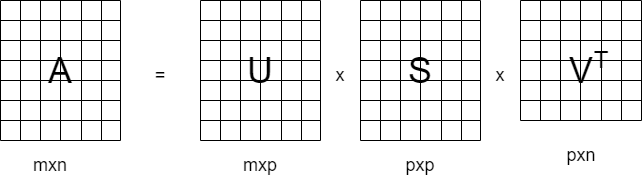
\includegraphics[width=0.8\textwidth]{Bilder_Stand_der_Technik/matrix_svd.png}}
    \caption{\label{figure:Matrix_SVD}\ac{SWZ}-Matrize}
\end{figure}
\noindent
Wobei m die Anzahl der Begriffe im Wörterbuch, n die Anzahl der Dokumente im Korpus und p die Summe der Themen im Korpus ist, die der Anzahl der Wörter entspricht.\\\\
Nach dem Theorem von Eckart-Young reduziert die \ac{SWZ} das Rauschen und die Spärlichkeit der ursprünglichen Matrix, indem sie durch eine Matrix derselben Dimensionalität, aber niedrigeren Rangs ersetzt wird, in der nur die wichtigsten Informationen erhalten bleiben. \cite{eckart_approximation_1936}\\\\
Die U-Matrix enthält die Term-Themen-Matrix. 
Sie wird auch als linke singuläre Vektormatrix bezeichnet, da sie die Zeilenvektoren enthält, die von links mit der Spaltenvektormatrix zu multiplizieren sind. 
Die U-Matrix spiegelt die gegenseitige Korrelation von Wörtern und Themen auf der Grundlage des gemeinsamen Auftretens von Wörtern im selben Dokument wider. 
Vor der Trunkierung (Entfernung der Spalten) ist sie quadratisch. 
Die Anzahl der Spalten und Zeilen in ihr entspricht der Anzahl der Wörter im Wörterbuch (m). 
Vor der Trunkierung ist die Anzahl der Themen (p) gleich der Anzahl der Wörter. 
Die U-Matrix enthält als Spalten Vektoren der Themen für alle Wörter des Korpus. 
Das bedeutet, dass sie verwendet werden kann, um einen Wort-Dokument-Vektor (\ac{TF-IDF}-Vektor oder \ac{BOW}-Vektor) in einen Themen-Dokument-Vektor umzuwandeln. 
Um einen neuen \glqq topic-document\grqq{}-Vektor zu erhalten, multipliziert man einfach die U-Matrix \glqq topic-word\grqq{} mit einem beliebigen \glqq word-document\grqq{}-Vektor. 
Der Punkt ist, dass die Gewichte (Scores) in den Zellen der U-Matrix die Bedeutung der Wörter für die Themen widerspiegeln.\\\\
Die quadratische diagonale S-Matrix (Sigma-Matrix) enthält die Singulärwerte (Eigenwerte) des Themas. 
Diese singulären Werte geben an, wie viel Information in jeder Dimension des neuen semantischen (Themen-)Vektorraums enthalten ist. 
In der diagonalen Matrix befinden sich Werte, die nicht Null sind, nur auf der Diagonalen von der linken oberen Ecke bis zur rechten unteren Ecke. 
Alle anderen Positionen in der S-Matrix enthalten Nullen. 
Und die Dimensionen (Themen) sind so angeordnet, dass die erste Dimension die meisten Informationen (erklärbare Varianz) über den Fall enthält. 
Wenn es also notwendig ist, das Themenmodell abzuschneiden, kann man mit den Messungen von unten rechts beginnen und sich nach links bewegen. 
Und dann aufhören, diese singulären Werte auf Null zu setzen, wenn der Fehler des thematischen Modells eine signifikante Auswirkung auf den Gesamtfehler der \ac{NLP}-Pipeline haben wird.\\\\
Die $V^{T}$-Matrix \glqq Dokument-Dokument\grqq{} enthält als Spalten die rechten singulären Vektoren und gibt Aufschluss über die gemeinsamen Bedeutungen von Dokumenten, da sie die Häufigkeit der Verwendung der gleichen Themen in Dokumenten in dem neuen semantischen Modell von Dokumenten misst. 
Es enthält so viele Zeilen (p) und Spalten, wie es Dokumente im Korpus gibt.\\\\
Nachdem die singuläre Zerlegung abgeschlossen ist, müssen die Themen so gekürzt werden, dass sie die Bedeutung der Dokumente wiedergeben. 
Dabei müssen die Elemente der Matrix S in absteigender Reihenfolge sortiert werden. 
In diesem Fall kann die Formel in einer anderen Form geschrieben werden:
\begin{equation}
    A_{k} = U_{k} S_{k} V_{k}^T
    \eqlabel{eq-trunkierte-swz}{Trunkierte SWZ-Matrix}
\end{equation}
Dabei sind $U_{k}$ und $V_{k}$ Matrizen, die durch Extraktion der ersten k Spalten aus den Matrizen U bzw. V gewonnen werden.
\begin{figure}[H]
    \centering
    \fbox{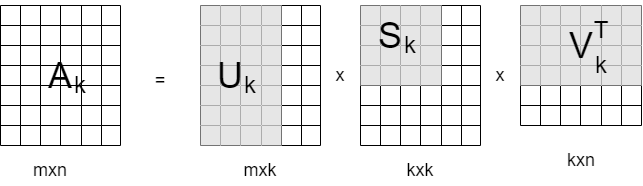
\includegraphics[width=0.8\textwidth]{Bilder_Stand_der_Technik/trun_svd.png}}
    \caption{\label{figure:Trun_SVD}Trunkierte \ac{SWZ}-Matrize}
\end{figure}
\noindent
Im latent-semantischen Modell kann also jeder Text und jeder Begriff durch Vektoren in einem reduzierten Raum der Dimension k - dem Themenraum - dargestellt werden. 
Diese \ac{SWZ} wird als parsimonious bezeichnet, weil sie in dem Fall, in dem k viel kleiner als m, n und p ist, eine erhebliche Kompression der ursprünglichen Information ermöglicht. 
Komprimierung ist in dem Sinne zu verstehen, dass ein Teil der von der ursprünglichen Matrix übermittelten Informationen verloren geht und nur die wichtigsten (dominanten) Informationen erhalten bleiben. 
Der Informationsverlust entsteht durch die Vernachlässigung kleiner Singulärzahlen. 
Je mehr Singulärzahlen verworfen werden, d. h. je kleiner k, desto größer ist dieser Verlust. 
Mit anderen Worten: Der Informationsverlust ist umso größer, je niedriger der Rang der approximierenden Matrix ist. 
In diesem Fall gehen zunächst die nicht signifikanten Werte verloren, wodurch die dominanten Werte der Matrix erhöht werden.\\\\
Der \ac{SWZ}-Algorithmus, das Herzstück von \ac{LSA}, erkennt, ob Wörter immer nebeneinander vorkommen und fasst sie im Betreff zusammen. 
Auf diese Weise kann er die Anzahl der Messungen ohne zusätzlichen Aufwand reduzieren. 
\ac{LSA} (\ac{SWZ}) ist eine großartige Methode, um Wort-Dokument-Matrizen zu komprimieren und potenzielle zusammengesetzte Wörter oder N-Gramme für die Pipeline zu erkennen. 
\ac{LSA} reduziert die Anzahl der Messungen und hilft so, Übertraining zu vermeiden. 
Sie führt eine Verallgemeinerung auf der Grundlage eines kleinen Datensatzes durch, indem sie eine lineare Beziehung zwischen den Worthäufigkeiten annimmt.\\\\
\ac{LSA}s können auch für die semantische Suche verwendet werden. 
Eine semantische Suche (semantic search) ist eine Art der Volltextsuche, die die Bedeutung der Wörter in der Anfrage und der gesuchten Dokumente berücksichtigt. 
Durch die Verwendung von Themenvektoren ist es möglich, die Bedeutung von Wörtern, Dokumenten, Aussagen und Korpora zu vergleichen. 
Es ist möglich, Cluster von ähnlichen Dokumenten und Aussagen zu finden. 
Mit Themenvektoren wird der Abstand zwischen Dokumenten nicht nur auf der Grundlage der in ihnen verwendeten Wörter betrachtet, sondern auf der Grundlage von Wörtern, die der Bedeutung entsprechen. 
Semantische Suchen mit Themenvektoren beschränken sich nicht nur auf die Suche nach Schlüsselwörtern und Relevanzrankings, die allein auf der Auswahl von Wörtern oder Vokabeln basieren. 
Sie können verwendet werden, um Dokumente zu finden, die für die Anfrage relevant sind, und nicht nur solche, die gut zu den Wortstatistiken passen. 
Dazu muss die Suchanfrage des Nutzers zunächst mit denselben Attributen vektorisiert werden wie die Dokumentenvektorisierung. 
Dann kann \ac{SWZ} verwendet werden, um die Dimensionalität des Abfragevektors auf die gleichen Dimensionen wie die der Dokumentvektoren zu reduzieren. 
Anschließend kann der Kosinuskoeffizient zwischen dem Abfragevektor und den Dokumentvektoren berechnet werden, um festzustellen, welche Dokumente der Abfrage am nächsten liegen. 
\ac{LSA} und \ac{SWZ} können also zum Aufspüren versteckter Themen in Textdokumenten sowie zur semantischen Suche in großen Dokumentensammlungen verwendet werden.\\\\
Es gibt viele Python-Bibliotheken und -Werkzeuge für die Implementierung von \ac{LSA} und \ac{SWZ}. 
Eine der beliebtesten Bibliotheken für Matrix- und Singulärzerlegung ist NumPy. 
NumPy erleichtert die Durchführung von Matrixoperationen und verfügt über eine Funktion zur Singulärzerlegung: \textit{numpy.linalg.svd()}. 
Zusammen mit anderen Bibliotheken wie \textit{Pandas} und \textit{Scikit-learn} kann \ac{LSA} effizient durchgeführt werden. 
Um \ac{LSA} zu starten, müssen die Textdaten mit Hilfe des \ac{TF-IDF}-Modells vektorisiert werden, wie zuvor beschrieben. 
Dann muss eine singuläre Zerlegung der Term-Dokument-Matrix mit \textit{numpy.linalg.svd()} durchgeführt werden. 
Danach kann eine bestimmte Anzahl von Hauptkomponenten (Topics) ausgewählt werden, die zur Darstellung der Dokumente verwendet werden. 
Dies kann durch die Auswahl der Komponenten mit den höchsten Singulärwerten geschehen. 
Anhand dieser Komponenten kann dann die Nähe zwischen den Dokumenten bestimmt werden.\\\\ 
\textit{Scikit-learn} bietet auch eine \textit{TruncatedSVD}-Klasse, mit der eine Truncated-\ac{SVD} durchgeführt werden kann, um nur die ausgewählten Hauptkomponenten zu erhalten. 
Diese Klasse erleichtert die Durchführung von \ac{LSA} auf großen Dokumentenkorpora und verfügt über zusätzliche Funktionen wie Datenverarbeitung und Normalisierung sowie automatische Auswahl der Anzahl der Komponenten auf der Grundlage des Prozentsatzes der erklärten Varianz.
\subsection{Ansätze für die Erstellung eines Chatbots}\label{sec:ansaetze_erstellung_chatbots}
Derzeit gibt es vier Hauptansätze für die Erstellung eines Chatbots \cite{lane_natural_2019}:
\begin{itemize}
    \item Musterabgleich: Musterabgleich und Antwortvorlagen (vorgefertigte Antworten)
    \item Grounding: logische Wissensgraphen und das Ziehen von Schlussfolgerungen aus diesen basierend auf diesen Graphen
    \item Suche: Abrufen von Text
    \item Generierungsmethoden: Statistik und maschinelles Lernen
\end{itemize}
Die vier grundlegenden Ansätze zur Erstellung von Chatbots lassen sich kombinieren, was zu benutzerfreundlicheren Chatbots führt. 
Eine Vielzahl von Anwendungen nutzen alle vier grundlegenden Methoden. 
Hybride Chatbots unterscheiden sich hauptsächlich darin, wie genau sie diese Ansätze kombinieren und wie viel Gewicht auf jeden einzelnen Ansatz gelegt wird.
\subsubsection{Musterabgleich}
Bei den ersten Chatbots basierte die Antwort auf die Nachricht eines Benutzers auf einem Mustervergleich. 
Diese Chatbots suchen nach Mustern im eingehenden Text und geben eine feste (gemusterte) Antwort, wenn eine Übereinstimmung gefunden wird \cite{woudenberg_chatbot_2014}.\\\\
Solche rudimentären Dialogsysteme sind vor allem in automatisierten Benutzerunterstützungssystemen mit interaktiven Sprachmenüs nützlich, wo es möglich ist, das Gespräch an einen Menschen weiterzuleiten, wenn der Chatbot keine Antwortmuster mehr hat.\\\\
Da es viele \ac{NLP}-Dienstprogramme in Python-Paketen gibt, ist es möglich, komplexere Chatbots auf der Grundlage von Mustervergleichen zu erstellen, indem man die Bot-Logik nach und nach direkt in Python mit regulären Ausdrücken und Suchmustern aufbaut.\\\\
1995 machte sich Richard Wallace daran, einen allgemeinen Rahmen für die Erstellung von Chatbots auf der Grundlage des Pattern-Matching-Ansatzes zu schaffen. Zwischen 1995 und 2002 schuf seine Entwicklergemeinschaft die \ac{AIML} zur Beschreibung von Mustern und Chatbot-Antworten.\\\\
\ac{AIML} ist eine deklarative Sprache, die auf dem \ac{XML}-Standard basiert, der die Sprachkonstrukte und Datenstrukturen einschränkt, die im Bot verwendet werden dürfen. \cite{noauthor_aiml_nodate}
Ein Chatbot, der auf \ac{AIML} basiert, sieht folgendermaßen aus:
\begin{figure}[H]
    \centering
    \fbox{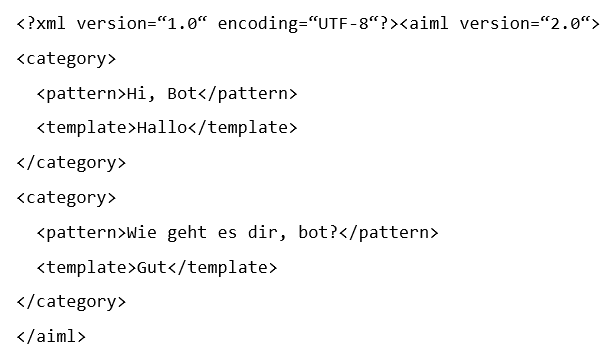
\includegraphics[width=0.8\textwidth]{Bilder_Stand_der_Technik/aiml_bot.png}}
    \caption{\label{figure:Aiml_Bot}\ac{AIML} Chatbot}
\end{figure}
\noindent
Eine der Einschränkungen von \ac{AIML} ist die Art der Muster, die abgeglichen werden können und auf die reagiert wird. 
Der \ac{AIML}-Kern (Pattern Matching Engine) reagiert nur auf Eingabetext, der einem vom Entwickler manuell vorgegebenen Muster entspricht. 
Unscharfe Suchanfragen, Smileys, Satzzeichen, Tippfehler oder falsch geschriebene Wörter sind nicht erlaubt, es findet kein automatischer Abgleich statt. 
In \ac{AIML} müssen alle Synonyme manuell einzeln beschrieben werden.
\subsubsection{Grounding}
Die Grounding-Methode ist ein Ansatz zur Erstellung eines Chatbots auf der Grundlage logischer Wissensgraphen und der Durchführung von Schlussfolgerungen auf der Grundlage dieser Graphen. \cite{diana_conversational_2011}
Sie wird verwendet, um natürliche Sprache zu verarbeiten und sie dem Verständnis des Bots zuzuordnen. Das Wesentliche an der Grounding-Methode ist, dass der Chatbot nicht nur die Textnachrichten, sondern auch den Kontext und die Umgebung verarbeitet, um Anfragen besser zu verstehen und zu beantworten. 
Durch die Extraktion von Informationen wird ein Netz von Verbindungen oder Fakten geschaffen. Dieses Netz logischer Verbindungen zwischen Entitäten - ein Graph oder eine Wissensbasis - kann die Grundlage für die Antworten des Chatbots bilden.\\\\
Ein Beispiel für eine Grounding-Methode ist die Verwendung eines Wissensgraphen zur Beschreibung der Umgebung. 
Ein Wissensgraph enthält Informationen über die Objekte, mit denen der Bot interagieren kann und die Beziehungen zwischen ihnen. 
Ein Wissensgraph könnte zum Beispiel Informationen über ein Glas auf einem Tisch und das darin befindliche Wasser enthalten. 
Wenn ein Benutzer eine Frage stellt, verwendet der Chatbot den Wissensgraphen, um den Kontext der Anfrage zu verstehen und die am besten geeignete Antwort abzuleiten. 
Wenn ein Benutzer zum Beispiel fragt: \glqq{}Wie hoch ist die Temperatur des Wassers in dem Glas auf dem Tisch?\grqq{}, kann der Chatbot Informationen aus dem Wissensgraphen verwenden, um die Frage zu beantworten.\\\\
Ein solcher Wissensgraph kann abgeleitet werden, um Fragen über die in dieser Wissensbasis enthaltene Welt zu beantworten und anschließend können auf der Grundlage der logischen Antworten die Werte der in den Antworten enthaltenen Template-Variablen ausgefüllt werden, um natürlichsprachliche Antworten zu erstellen. 
Ursprünglich wurden auf diese Weise Systeme zur Beantwortung von Fragen eingerichtet, wie z. B. der Watson-Bot von IBM (heutzutage wird für ähnliche Systeme jedoch die Informationssuchemethode verwendet). 
Der Wissensgraph stellt eine Art \glqq{}Erdung\grqq{} des Chatbots in der realen Welt dar.\\\\
Die Erstellung von Chatbots auf der Grundlage von \glqq{}Grounding\grqq{} eignet sich hervorragend für Chatbots, die Fragen generieren, bei denen das zur Beantwortung einer Frage erforderliche Wissen in einer umfangreichen Wissensbasis enthalten ist, die aus einer offenen Datenbank (z. B. Wikidata, Open Mind Common Sense oder DBpedia) bezogen werden kann.\\\\
Einer der Hauptvorteile der Grounding-Methode besteht darin, dass sie sich an ein sich veränderndes Umfeld anpassen kann. 
Wenn der Benutzer zum Beispiel ein Glas Wasser von einem Tisch auf einen anderen stellt, wird der Wissensgraph automatisch aktualisiert, um diese Änderung widerzuspiegeln.\\\\
Die Grounding-Methode hat jedoch auch ihre Grenzen. 
So kann es vorkommen, dass bei der Verarbeitung großer Informationsmengen Zusammenhänge nicht berücksichtigt werden und dem Bot möglicherweise verborgen bleiben.\\\\
Insgesamt ist die Grounding-Methode ein effektiver Ansatz zur Erstellung wissensbasierter Chatbots. 
Sie ermöglicht es dem Bot, Benutzeranfragen besser zu verstehen und eine genauere Antwort zu geben.
\subsubsection{Suche}
Die Informationssuchemethode ist eine der Methoden zum Aufbau von Chatbots, die auf der Extraktion von Informationen aus einer großen Menge von Textinformationen basiert. 
Die Hauptidee der Informationssuchemethode ist die Analyse des Eingabetextes (Benutzeranfrage), die Auswahl von Schlüsselwörtern und Phrasen daraus und die anschließende Suche nach den relevantesten Informationen in der Wissensdatenbank oder in offenen Quellen. \cite{diana_conversational_2011}\\\\
Die Wissensbasis kann auch eine Art \glqq{}Gesprächsprotokoll\grqq{} sein, in Form von Aussage-Antwort-Paaren. 
Dabei sucht der Bot nach früheren Aussagen in den Protokollen früherer Unterhaltungen. 
Der Bot kann nicht nur in den Protokollen seiner eigenen Gespräche suchen, sondern auch in beliebigen Transkripten von Gesprächen zwischen Menschen, Gesprächen zwischen Menschen und Bots oder sogar Gesprächen zwischen Bots.
Aber wie immer gilt: je besser die Eingabedaten, desto besser das Ergebnis. 
Daher ist es notwendig, die Datenbank früherer Gespräche sorgfältig zu säubern und zu organisieren, damit der Bot nach einem qualitativ hochwertigen Gespräch sucht und es dann imitiert.\\\\
Für die Umsetzung der Informationssuchemethode werden verschiedene Algorithmen und Techniken verwendet, z. B. Indizierung und Schlagwortsuche, Kontextsuche, Textanalyse mit Hilfe von maschinellen Lernverfahren usw. 
Die Informationssuchemethode kann in Python mit verschiedenen Bibliotheken und Tools wie \ac{NLTK}, Scikit-learn und Gensim implementiert werden.\\\\
Einer der ersten Schritte bei der Implementierung einer Informationssuchemethode in Python ist die Vorbereitung der Daten. 
Dies erfordert Tokenisierung, Lemmatisierung und die Entfernung von Stopp-Wörtern. 
Als nächstes muss ein Index auf der Grundlage von Schlüsselwörtern erstellt werden. 
Der Index kann auf der Grundlage von Bag-of-Words oder \ac{TF} und \ac{IDF} (TF-IDF-Modelle) erstellt werden. 
Sobald der Index erstellt ist, kann eine Stichwortsuche durchgeführt werden. 
Dazu muss die Benutzeranfrage in einen Vektor umgewandelt und mit den Dokumentvektoren im Index verglichen werden. 
Dies kann mit Hilfe der Scikit-learn-Bibliothek erfolgen \cite{scikit-learn}.
Sobald die relevantesten Dokumente gefunden wurden, können sie in eine Rangfolge gebracht und als Antwort auf die Benutzeranfrage angezeigt werden.\\\\
Der Vorteil der Informationssuchemethode besteht darin, dass sie ein schnelles und genaues Auffinden der gewünschten Informationen ermöglicht, insbesondere wenn die Wissensbasis gut strukturiert ist und genügend Informationen enthält. 
Ein Nachteil dieser Methode ist jedoch, dass sie den Kontext der Anfrage nicht berücksichtigt und nicht immer eine vollständige und genaue Antwort auf die Frage des Nutzers liefert. 
Wenn die Aussage semantisch mit der vom Bot zu beantwortenden übereinstimmt, ist es möglich, die Antwort wortwörtlich und ohne Änderungen wiederzuverwenden. 
Aber selbst wenn die Datenbank alle möglichen Benutzeräußerungen enthält, wird der Bot die Persönlichkeiten der Personen widerspiegeln, die diese Äußerungen machen. 
Wenn die Antworten konsistent sind und von einer Vielzahl von Personen stammen, ist das gut. 
Problematisch wird es jedoch, wenn die Äußerung, auf die der Bot reagieren soll, vom Gesamtkontext des jeweiligen Gesprächs oder von den Umständen in der Umgebung abhängt, die sich seit der Erstellung des Dialogkorpus geändert haben können.\\\\
Beispielsweise sollte der Bot auf die Frage \glqq{}Wie spät ist es?\grqq{} nicht die von der Person gegebene Antwort, sondern die am besten geeignete Aussage aus der Datenbank verwenden. 
Diese Antwort funktioniert nur, wenn die Zeit, zu der die Frage gestellt wurde, mit der Zeit übereinstimmt, zu der die passende Äußerung aus der Datenbank aufgezeichnet wurde. 
Neben dem natürlichsprachlichen Text der Äußerung müssen auch ähnliche Informationen über die Zeit - der Kontext (Zustand) - erfasst und verglichen werden. 
Sie spielt vor allem dann eine wichtige Rolle, wenn die Semantik der Äußerung auf eine aktive Veränderung des im Kontext (Wissensbasis des Chatbots) erfassten Zustands hinweist.\\\\
Um den Zustand (Kontext) in einem Chatbot auf der Grundlage der Informationssuche zu berücksichtigen, kann etwas Ähnliches für einen Chatbot mit Musterabgleich durchgeführt werden, da die Auflistung einer Liste von Benutzeraussagen nur eine andere Art ist, ein Muster zu beschreiben. 
Dies auch ist der Ansatz von Amazon Lex \cite{amazon_lex} und Google Dialogflow \cite{dialogflow_chawla}. 
Anstatt ein starres Muster zu beschreiben, um den Befehl des Benutzers zu erfassen, können der Dialogflow-Engine einfach ein paar Beispiele geliefert werden. 
So wie jedes Muster im Chatbot auf der Grundlage der Musterzuordnung einem Zustand zugeordnet wurde, muss auch hier nur die Aussage-Antwort-Beispielpaare mit dem genannten Zustand verknüpft werden.\\\\
Der suchbasierte Chatbot indiziert also den Korpus der Dialoge, so dass er leicht frühere Aussagen finden kann, die derjenigen ähnlich sind, auf die er antworten muss und antwortet dann mit einer der passenden Aussagen aus dem Korpus, die er sich \glqq{}gemerkt\grqq{} und für eine schnelle Suche indiziert hat. 
Im Allgemeinen ist die Methode der Informationssuche eine der gängigsten und beliebtesten Methoden zum Aufbau von Chatbots, die in verschiedenen Bereichen wie Wirtschaft, Medizin, Tourismus und vielen anderen eingesetzt werden.
\subsubsection{Generierungsmethoden}
Generierungsmethoden sind einer der wichtigsten Ansätze bei der Entwicklung von Chatbots auf der Grundlage künstlicher Intelligenz. 
Sie ermöglichen es Chatbots, Textantworten auf der Grundlage der Analyse der eingehenden Nachricht und des Kontextes des Dialogs zu generieren. 
Die folgenden Generierungsmodelle sind nützlich, um einen kreativen Chatbot zu erstellen, der Dinge sagen kann, die noch niemand zuvor gesagt hat:
\begin{itemize}
    \item Sequenz-zu-Sequenz-Konvertierungsmodelle: Modelle, die darauf trainiert sind, Antworten auf der Grundlage von Eingabesequenzen zu generieren;
    \item \ac{RBM}: Markov-Ketten, die so trainiert werden, dass sie die \glqq{}Energie\grqq{}-Funktion minimieren \cite{chatbot_development_sharma};
    \item \ac{GAN}: statistische Modelle, die darauf trainiert sind, einen Experten, der die Qualität eines Gesprächs bewertet, zu täuschen. \cite{li_adversarial_2017}
\end{itemize}
Die Vorteile des Einsatzes der Generierungsmethoden:
\begin{itemize}
    \item Flexibilität: Generative Methoden können für eine breite Palette von Aufgaben eingesetzt werden, einschließlich Texterstellung, Sprachübersetzung, Verarbeitung natürlicher Sprache und mehr.
    \item Automatisierung: Generative Methoden können auf großen Datensätzen trainiert werden, wodurch die Erstellung von Inhalten automatisiert werden kann.
    \item Qualität: Generative Methoden zeigen eine hohe Qualität bei der Textgenerierung, Sprachübersetzung und anderen Aufgaben der natürlichen Sprachverarbeitung, wenn sie auf einem ausreichend großen Datensatz trainiert werden.
    \item Schnelligkeit: Generative Methoden können schneller arbeiten als Menschen, was die Erstellung von Inhalten mit großer Geschwindigkeit ermöglicht.
\end{itemize}
Die Nachteile der generativen Methoden:
\begin{itemize}
    \item Große Datenmengen für das Training: Generative Methoden benötigen große Datenmengen für das Training, was bei einigen Aufgaben schwierig sein kann, insbesondere wenn nur ein kleiner Datensatz zur Verfügung steht.
    \item Sicherheitsrisiken: Generative Methoden können Inhalte erzeugen, die möglicherweise falsch, unvollständig oder irreführend sind. Dies kann zu Sicherheitsrisiken führen, wenn der generierte Inhalt für wichtige Entscheidungen verwendet wird.
    \item Unterstützungsbedarf: Generative Methoden können erhebliche Unterstützung benötigen, um effektiv zu sein. Dies kann die Modellabstimmung, die Auswahl optimaler Parameter und die Optimierung der Modellleistung auf einer bestimmten Hardwarekonfiguration umfassen.
    \item Modellbeschränkungen: Generative Methoden können Beschränkungen hinsichtlich der Arten von Inhalten haben, die sie erzeugen können, insbesondere wenn sie nur auf bestimmte Datentypen trainiert wurden.
\end{itemize}
Eine der beliebtesten Methoden zur Texterstellung ist die sequence-to-sequence-Methode (seq2seq). 
Die seq2seq-Methode basiert auf \ac{RNN}, die die Simulation von Datenfolgen ermöglichen. 
Sie besteht aus zwei Hauptteilen: einem Encoder und einem Decoder. 
Ein Encoder empfängt eine Wortfolge und baut daraus einen Kontextvektor auf, der Informationen über die Eingabedaten enthält. 
Der Decoder erhält diesen Vektor als Eingabe und beginnt mit der Generierung einer Folge von Antwortnachrichten, wobei er schrittweise den Kontext und die zuvor generierten Wörter berücksichtigt. \cite{seq2seq_alammar}\\\\
Einer der Hauptvorteile der seq2seq-Methode ist ihre Fähigkeit, qualitative und grammatikalisch korrekte Textantworten zu generieren, einschließlich Antworten, die nicht in den Trainingsdaten enthalten waren. 
Sie kann auch mit langen Sequenzen umgehen, was sie ideal für die Generierung von Antworten in Dialogsystemen macht. 
Darüber hinaus kann die seq2seq-Methode in einer Vielzahl von Anwendungen eingesetzt werden, z. B. in der maschinellen Übersetzung, der Spracherkennung und anderen.\\\\
Die seq2seq-Methode hat jedoch ihre Nachteile. 
Sie erfordert große Datenmengen zum Trainieren und Verarbeiten sowie erhebliche Rechenressourcen. 
Dies kann die Anwendung der Methode bei einigen Anwendungen einschränken. 
Wenn der Trainingsdatensatz nicht eine ausreichend große Bandbreite möglicher Antworten repräsentiert, kann das Modell außerdem dazu neigen, vorhersehbare oder falsche Antworten zu erzeugen.\\\\
Die Implementierung der seq2seq-Methode in Python kann mit der TensorFlow-Bibliothek erfolgen, die eine Reihe von Werkzeugen für den Aufbau und das Training neuronaler Netze bietet. 
In TensorFlow kann man die vortrainierten seq2seq-Modelle verwenden oder ein eigenes Modell erstellen, indem die Architektur und die Trainingsparameter des Netzwerks konfiguriert wird. \cite{tensorflow}
\subsection{Mehrschichtiges Perzeptron für ein Mehrklassen-Klassifizierungsproblem}
Ein \ac{MLP} ist eine neuronale Netzwerkarchitektur, die aus mehreren Schichten von Neuronen besteht und für Klassifizierungs- und Regressionsaufgaben verwendet werden kann. 
Mehrschichtige Perzeptronen sind Arten von neuronalen Netzen, die bidirektional sind, da sie die Eingabedaten vorverteilen und die Gewichte zurückverteilen. 
Ein mehrschichtiges Perzeptron hat eine Eingabeschicht und eine Ausgabeschicht mit einer oder mehreren versteckten Schichten. 
Bei \ac{MLP} sind alle Neuronen einer Schicht mit allen Neuronen der nächsten Schicht verbunden. 
Die Eingabeschicht empfängt Eingangssignale und die gewünschte Aufgabe wird von der Ausgabeschicht ausgeführt. 
Die versteckten Schichten sind für alle Berechnungen zuständig. 
Die Architektur des mehrschichtigen Perzeptrons sieht folgendermaßen aus:
\begin{figure}[H]
    \centering
    \fbox{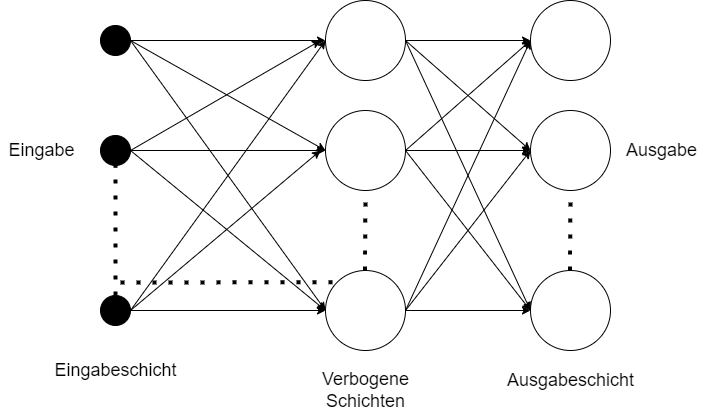
\includegraphics[width=0.8\textwidth]{Bilder_Stand_der_Technik/mehrschicht_perc.png}}
    \caption{\label{figure:Mehrschichtiges_Perzeptron}Mehrschichtiges Perzeptron}
\end{figure}
\noindent
Für ein Mehrklassen-Klassifizierungsproblem kann ein \ac{MLP} mit einer Verlustfunktion wie der kategorialen Kreuzentropie (Categorical Crossentropy) trainiert werden. 
Zunächst muss ein \ac{MLP} über eine Eingabeschicht verfügen, die die Merkmale eines Objekts aufnimmt, und eine Ausgabeschicht, die die Wahrscheinlichkeiten für die Zugehörigkeit des Objekts zu den einzelnen Klassen ausgibt. 
Die Dimensionalität der Ausgabeschicht muss der Anzahl der zu klassifizierenden Klassen entsprechen.
Außerdem können zwischen der Eingabe- und der Ausgabeschicht mehrere verborgene Schichten liegen, die nichtlineare Transformationen der Eingabedaten durchführen, so dass das \ac{MLP}-Modell komplexe Beziehungen zwischen Objektmerkmalen und Klassen erfassen kann. 
Jedes Neuron im \ac{MLP} nimmt als Eingabe die gewichtete Summe der Neuronenausgaben der vorherigen Schicht, fügt eine Vorspannung hinzu und durchläuft dann eine Aktivierungsfunktion. 
Die Aktivierungsfunktion wird verwendet, um dem \ac{MLP} Nichtlinearität hinzuzufügen und kann z. B. sigmoid-Funktion oder ReLU sein.
Beim \ac{MLP}-Training mit Gradientenabstieg werden die Gewichte und Vorspannungen der Neuronen bei jeder Trainingsiteration aktualisiert, wobei der Wert der Verlustfunktion minimiert wird.\\\\
Die kategoriale Kreuzentropie ist eine Verlustfunktion, die für die Klassifizierung mehrerer Klassen verwendet wird und die Diskrepanz zwischen den wahren Klassenbezeichnungen und den vorhergesagten Klassenwahrscheinlichkeiten misst. 
Daher kann \ac{MLP} nach dem Training zur Klassifizierung neuer Objekte verwendet werden, indem die Objektmerkmale durch \ac{MLP} geleitet werden und die Ausgabewahrscheinlichkeiten für jede Klasse ermittelt werden und dann die Klasse mit der höchsten Wahrscheinlichkeit als vorhergesagte Klassenbezeichnung ausgewählt wird.\\\\
Die Theorie hinter der kategorialen Kreuzentropie ist die Informationstheorie und die Messung der Unsicherheit. 
Angenommen, es gibt ein System, das mit einem probabilistischen Modell beschreiben werden muss. 
Dieses System habe N mögliche Ergebnisse, die jeweils mit den Wahrscheinlichkeiten $p_{1}$, $p_{2}$, ..., $p_{N}$ auftreten können, wobei $\sum_i p_i = 1$ und $p_i\geq0$ für i = 1, 2, ..., N. 
Dann kann die Entropie H des Systems wie folgt definiert werden: 
\begin{equation}
    H = -\sum (p_{i}*\log_{2}{p_{i}})
    \eqlabel{eq-entropie}{Entropie H}
\end{equation}
Dabei wird $\sum$($p_{i}$* $\log_{2}{p_{i}}$) über i von 1 bis N genommen \cite{koech_cross-entropy_2022}. 
Diese Formel zeigt, dass die Entropie des Systems ein Maß für die Ungewissheit oder Unsicherheit bei der Wahl eines der möglichen Ergebnisse ist.\\\\
Wenn die kategoriale Kreuzentropie als Verlustfunktion für ein Mehrklassen-Klassifizierungsproblem verwendet wird, wird erwartet, dass das trainierte Modell einen Ausgabewahrscheinlichkeitsvektor hat, bei dem jedes Element des Vektors einer der Klassen entspricht. 
Je unsicherer der Modellausgabevektor für ein bestimmtes Beispiel ist, desto höher ist der Wert der kategorialen Kreuzentropie. 
Umgekehrt ist der Wert der kategorialen Kreuzentropie gleich Null, wenn das Modell eine Klasse für ein bestimmtes Beispiel genau vorhersagt.
Beim Training von Klassifizierungsmodellen für Aufgaben des maschinellen Lernens mit mehreren Klassen wird daher versucht, den Wert der kategorialen Kreuzentropie zwischen dem Ausgabevektor des Modells und der richtigen Klasse für jedes Eingabebeispiel zu minimieren. 
Zu diesem Zweck wird ein Optimierungsverfahren verwendet, z. B. den Gradientenabstieg, um die Gewichte und Verzerrungen des Modells bei jeder Trainingsiteration zu aktualisieren.\\\\
In Keras kann die kategoriale Kreuzentropie als Verlustfunktion für verschiedene Modelltypen wie mehrschichtige Perzeptronen, faltungsneuronale Netze und rekurrente neuronale Netze verwendet werden. 
Es handelt sich um eine Standardverlustfunktion für Mehrklassen-Klassifizierungsprobleme. 
Bei der Verwendung der kategorialen Kreuzentropie in Keras können auch verschiedene Parameter wie Klassengewichte und Modellbewertungsmetriken angepasst werden, um genauere Klassifizierungsergebnisse zu erhalten. 
Somit ist die kategoriale Kreuzentropie ein wichtiges Werkzeug beim maschinellen Lernen zur Lösung von Klassifizierungsproblemen mit mehreren Klassen. 
Ihre Verwendung ermöglicht es, Modelle zu trainieren, die Eingabebeispiele genau klassifizieren und eine hohe Genauigkeit bei Klassifizierungsaufgaben erreichen können.

\endinput
\chapter{Anforderungen} \label{chap:Anforderungen}
Im Folgenden sollen die Anforderungen an das Ergebnis der Arbeit konkretisiert werden.
\section{Antwortzeit}
Diese Eigenschaft beschreibt die Zeitdauer vom registrieren eines Sprachbefehls bis zur Ausführung des Befehls durch die Mischmaschine und das Zurückgeben einer Antwort an den Benutzer. Die Antwortzeit spielt eine große Rolle bei der Bedienbarkeit eines interaktiven Systems, um das es sich bei der Mischmaschine handelt. Zu lange Antwortzeiten können dazu führen, dass der Benutzer seine ursprünglichen Ziele vergisst oder in Stress gerät, da in den aller meisten Fällen der Grund für eine lange Antwortzeit vor dem Benutzer verborgen bleibt. Umgekehrt können zu kurze Antwortzeiten ebenfalls zu Stress und Fehlbedienung seitens des Benutzers führen. Dies liegt unter anderem daran, dass kurze Antwortzeiten den Benutzer dazu veranlassen weniger über seine Aktionen und deren Folgen nachzudenken. Als eine für viele Anwendungen geeignete Antwortzeit werden zwei bis vier Sekunden genannt \cite{herczeg_9_2018}. Als maximale tolerierbare Antwortzeit werden für dieses Projekt sechs Sekunden festgelegt. Diese vergleichsweise lange Zeitdauer lässt sich zum Einen mit den langwierigen aber notwendigen Berechnungen begründen, die für die Spracherkennung und -verarbeitung benötigt werden. Zum Anderen werden die Auswirkungen einer langen Antwortzeit als gering eingeschätzt, da der Benutzer für diese Anwendung keine Teilarbeitsschritte o. ä. im Gedächtnis behalten muss. Das Ziel des Benutzers sich ein Getränk zubereiten zu lassen ist nach dem Eingang des Sprachbefehls bereits erfüllt.
\section{Offline-Funktionalität}
Die Mischmaschine sollte für die Sprachsteuerung keine Verbindung zum Internet benötigen, da dies die möglichen Einsatzorte der Maschine deutlich einschränken würde.  Diese Anforderung schränkt die möglichen, einzusetzenden Technologien zur Spracherkennung und -verarbeitung stark ein, da keine Cloud-Services wie bspw. \textit{Google Cloud Speech} eingesetzt werden können \cite{google_cloud_speech}. Eine weitere Herausforderung die dadurch entsteht ist, dass Berechnungen die unter Umständen sehr aufwendig sein können nicht ausgelagert sondern auf der Hardware innerhalb der Mischmaschine ausgeführt werden müssen.
\section{Lautstärke}
Die Lautstärke der, von der Mischmaschine zurückgegebenen Antwort, muss laut genug sein, sodass sie vom Benutzer gut verstanden werden kann. Diese Eigenschaft schränkt die Art und Weise wie die Hardware (Computer und Mikrofon) in die Mischmaschine eingebaut werden kann ein und welche Art von Hardware überhaupt verwendet werden kann.
\section{Entfernung}
Mit dieser Eigenschaft ist die Entfernung des Anwenders zu der Mischmaschine gemeint. Es muss dem Anwender ermöglicht werden aus einer moderaten Entfernung mit der Mischmaschine über die Sprachsteuerung zu interagieren. Sowohl die Eingabe eines Befehls über die Sprachsteuerung als auch die zu hörende Antwort sollte mindestens aus einer Entfernung von einem Meter möglich sein. Dafür müssen die Lautsprecher eine bestimmte Lautstärke erreichen können und das Mikrofon eine moderate Empfindlichkeit aufweisen.
\section{Antworten}
Die Antworten, die durch die Mischmaschine an den Benutzer zurückgegeben werden, sollen mit Hilfe eines eigens erstellten Sprachmodells auf Basis von künstlicher Intelligenz und \ac{ML} erfolgen. Die Antworten der Mischmaschine sollen außerdem bissiger bzw. sarkastischer Natur sein was, je nach verwandter Technik, bei der Auswahl der Trainingsdaten eine große Rolle spielt.\\\\
Des Weiteren bestehen die Anforderungen, dass der Benutzer auf Deutsch mit der Mischmaschine kommunizieren können muss und die Antworten der Mischmaschine kontrollierbar sein müssen. Mit der Kontrollierbarkeit ist gemeint, dass Vorhersagen darüber gemacht werden können, was die Mischmaschine in Etwa auf eine bestimmte Frage oder sonstige Benutzereingabe antworten wird. Dies soll verhindern, dass der Benutzer von unerwarteten Reaktionen seitens der Maschine überrascht wird und die Antwroten der Maschine den Benutzer nicht beleidigen (aufgrund der sarkastischen bzw. humorvollen Art und Weise, wie die Maschine antworten soll).     
\section{Kosten}
Die Materialkosten sollten einen gewissen Maximalbetrag nicht überschreiten. Zu den benötigten Materialien zählen ein Mikrocomputer zur Durchführung der Spracherkennung und -verarbeitung, ein Mikrofon zur Aufnahme der Sprache und Lautsprecher zur Tonausgabe. Das Ziel besteht darin einen Betrag von 200€ nicht zu überschreiten.
\section{Verbrauch von Arbeits- und Festplattenspeicher}
Diese Anforderung korreliert mit der Anforderung nach Offline-Funktionalität. Diese bedingt, dass aufwendige, rechen- oder speicherintensive Operationen nicht auf entfernte Rechner ausgelagert werden können sondern, alles auf \glqq{}kleiner\grqq{} Hardware innerhalb der Mischmaschine ablaufen muss. Diese Einschränkung soll anhand eines konkreten Beispiels verdeutlicht werden. Die vierte Version der bekannten Mikrocomputerreihe \textit{Raspberry Pi} umfasst im Modell B maximal acht Gigabyte \ac{RAM} und einen Micro-SD-Karten-Steckplatz \cite{ltd_raspberry_nodate}. Zwar sind Micro-SD-Karten von bis zu mehreren hundert Gigabyte erhältlich, jedoch muss dabei der Kostenfaktor mit beachtet werden. Dadurch sind sowohl Primär- als auch Sekundärspeicher stark beschränkt.\\\\
Auch Prozessorgeschwindigkeit und Grafikkartenleistung können bei der Spracherkennung- und verarbeitung eine Rolle spielen. Diese ist bei Mikrocomputern ebenfalls eingeschränkt und korreliert negativ mit der Anforderung an Geschwindigkeit. Einen ebenso negativen Einfluss auf die Geschwindigkeit des Gesamtsystems haben die virtuelle Vergrößerung des \ac{RAM} durch Swapping oder die SD-Karte selbst, welche im Vergleich mit anderen Speichertechnologien in Sachen Geschwindigkeit deutlich das Nachsehen hat.\\\\
In anbetracht der geschilderten Herausfoderungen und Kostenbetrachtung wird der maximal zu verbrauchende Arbeits- und Festplattenspeicher für dieses Projekt auf acht Gigabyte \ac{RAM} und 20 Gigabyte Festplattenspeicher festgelegt.
\section{Anpassungsfähigkeit}
Diese Anforderung beschreibt den Grad der Einfachheit bei Änderung der Anforderungen oder Umwelt die Sprachsteuerung der Mischmaschine an diese neuen Begebenheiten anzupassen. Ein einfaches Beispiel für die Anpassungsfähigkeit des Systems wäre das Hinzukommen eines Behälters innerhalb der Mischmaschine. Tritt dieser Fall ein sollte es leicht möglich sein die Sprachsteuerung so anzupassen, dass der Benutzer auch die Möglichkeit bekommt aus dem neuen, fünften Behälter Getränke zu Mischen und zu Bestellen. 
\section{Bewertung der Ansätze zur Erstellung eines Dialogsystems}
Unter Berücksichtigung der genannten Anforderungen und der im Kapitel \ref{sec:ansaetze_erstellung_chatbots} besprochenen Ansätze zur Erstellung eines Dyalogsystems, können die folgenden Schlussfolgerungen gezogen werden, ob die Ansätze den Anforderungen entsprechen oder nicht:
\begin{table}[H]
    \centering
    \begin{tabular}{l|c|c|c|c}
        \makecell{Ansatz/\\Anforderung} & Musterabgleich & Grounding & Suche & \makecell[l]{Generierungs-\\methoden} \\
        \hline
        \makecell{Antwortzeit} & entspricht  & entspricht nicht & entspricht & entspricht nicht \\
        \hline
        \makecell{Offline-\\Funktionalität}            & entspricht             & entspricht      & entspricht   & entspricht \\
        \hline
        \makecell{Sarkastische \\Antworten} & entspricht      & entspricht & entspricht & entspricht nicht   \\
        \hline
        \makecell{Antworten \\auf deutsch}                & entspricht     & entspricht nicht    & entspricht nicht    & entspricht nicht \\
        \hline
        \makecell{kontrollierbare \\Antworten}                  & entspricht             & entspricht      & entspricht & entspricht nicht   \\
        \hline
        \makecell{Verbrauch von \\Arbeits- und \\Festplattenspeicher}             & entspricht             & entspricht nicht      & entspricht nicht & entspricht nicht   \\
    \end{tabular}
    \caption{\label{table:Bewertungsmatrix_Anforderungen_Dialogsystem}Bewertung der Ansätze zur Erstellung eines Dialodsystems}
\end{table}
\noindent
\endinput
\chapter{Konzept} \label{chap:konzept}
In diesem Kapitel wird zunächst erläutert, wie die Steuerung der Getränkemischmaschine durch Sprachbefehle im Allgemeinen ablaufen wird.
Anschließend werden mehrere Konzepte vorgestellt, die das allgemeine Konzept konkretisieren.
Diese werden anhand der, in Kapitel \ref{section:Bewertungskriterien} erläuterten Kriterien, bewertet.
Zuletzt wird die Wahl des finalen Konzepts begründet.
\section{Allgemein}
Der Benutzer soll über Spracheingaben mit der Mischmaschine interagieren können.
Dafür muss das Gesprochene zunächst durch ein Mikrofon aufgenommen werden.
Anschließend können die Audiosignale weiterverarbeitet werden.
Der Benutzer soll hierbei nicht auf fest vorgegebene Sprachbefehle beschränkt sein, sondern für nahezu jede Eingabe eine sinnvolle Antwort zurückerhalten.
Um dies zu gewährleisten wird die Spracheingabe durch ein Sprachmodell, welches mittels maschinellen Lernverfahren trainiert wurde, verarbeitet.
Ergebnisse dieser Verarbeitung sind die Antwort, die an den Benutzer zurückgegeben wird, und ein konkreter Befehl für die Mischmaschine.
Ein Beispiel für einen solchen Befehl könnte etwa die Zubereitung eines bestimmten Getränks sein.
Für die Ausgabe einer Antwort ist ein Lautsprecher notwendig.
Denkbar wäre auch eine textbasierte Ausgabe, allerdings ginge damit der Eindruck des Benutzers verloren eine echte Konversation mit der Mischmaschine zu führen.
Das Sprachmodell mit der Getränkemischmaschine zu verknüpfen stellt eine Herausforderung dieser Arbeit dar.
\section{Bewertungskriterien} \label{section:Bewertungskriterien}
Im Folgenden sind die Bewertungskriterien für die einzelnen Konzepte aufgelistet:
\begin{itemize}
    \item Freiheitsgrade in der Spracheingabe des Benutzers: Erhält der Benutzer passende Antworten zurück egal was er sagt oder ist er auf einige wenige Befehle beschränkt?
    \item Hardwarekosten: Wie kostspielig ist das Konzept bezüglich der zusätzlich benötigten Hardware?
    \item Verfügbare Rechenleistung: Wie hoch ist die Verfügbare Rechenleistung im Vergleich zu den anderen Konzepten? Reicht diese aus um das Sprachmodell auszuführen?
    \item Performanz: Als wie performant wird die Lösung eingeschätzt? Ist mit Latenzen zwischen der Einagbe des Benutzers, der Ausgabe einer Antwort und Ausführung der Aktion zu rechnen?
    \item Overhead: Wie hoch ist im Allgemeinen der Mehraufwand einzuschätzen?
\end{itemize}
\section{Konzept A: Spracherkennung und -verarbeitung mittels Arduino} \label{section:Konzept_A}
Ein erstes Konzept sieht vor, dass das Audiosignal direkt von einem der Arduinos in der Getränkemischmaschine aufgenommen wird.
Das Audiosignal wird vom Arduino interpretiert und eine passende Antwort wird ausgegeben.
Außerdem sendet der Arduino die entsprechenden Signale, um die vom Benutzer gewünschte Aktion von der Getränkemischmaschine ausführen zu lassen.
Ein Problem ist hierbei die Interpretation des Audiosignals durch den Arduino, da dessen Leistung nicht für das Ausführen eines Sprachmodells ausreicht.
Folglich muss dieser Prozess ausgelagert werden.
Das Konzept wird deshalb um ein cloudbasiertes Sprachverarbeitungssystem ergänzt, welches den Sprachbefehl des Benutzers vom Arduino entgegennimmt und einen passenden Befehl und eine passende Antwort zurückgibt (s. Abb. \ref{figure:Spracherkennung_mittels_Arduino}).
Die Kommunikation zwischen Arduino und Cloudsystem kann über das \ac{HTTP} erfolgen.
\begin{figure}[H]
    \centering
    % \includegraphics does not allow jpg images apparently!
    \fbox{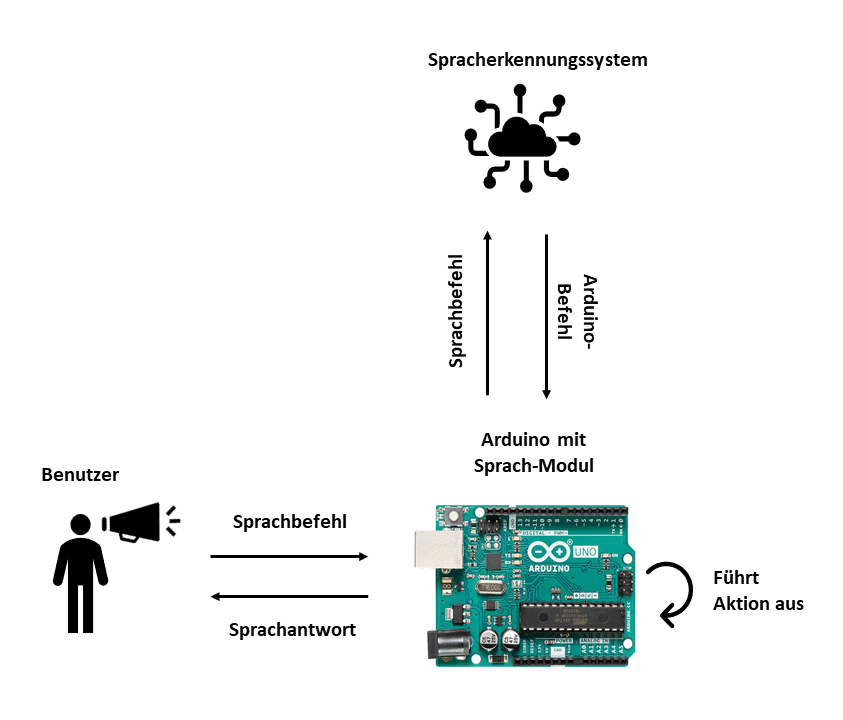
\includegraphics[width=0.8\textwidth]{Bilder_Konzept/Konzept_A.png}}
    \caption{\label{figure:Spracherkennung_mittels_Arduino}Spracherkennung und -verarbeitung mittels Arduino}
\end{figure}
\noindent
Es muss ein geeignetes Format zum Versenden des Sprachbefehls über \ac{HTTP} gefunden werden.
Eine Möglichkeit besteht darin, das eingehende Audiosignal im Arduino in textform umzuwandeln und diesen String zu versenden.
Die auf dem Markt verfügbaren Arduino-Sprach-Module sind jedoch nicht in der Lage beliebige Spracheingaben in Text umzuwandeln, sondern bieten diese Funktionalität nur für vordefinierte Werte an.
Dies würde das Ziel dieser Arbeit verfehlen, dem Benutzer eine Konversation mit der Mischmaschine zu ermöglichen.
Ein weiteres Problem dieser Lösung besteht darin, dass beispielsweise bei wechselnder Getränkeauswahl die zur Verfügung stehenden Sprachbefehle wie "`Ich hätte gerne Getränk xy"' jedes Mal aufs neue manuell angepasst werden müssten.
Dies hat zur Folge, dass auch die reine Spracherkennung aus der Mischmaschine ausgelagert werden muss.
Ein denkbares Format sind die rohen Audiosignale, die vom Arduino aufgenommen werden.
\section{Konzept B: Spracherkennung und -verarbeitung mittels mobiler Anwendung}
Die Audiosignale über ein Mikrofon in der Mischmaschine aufzunehmen und eine Antwort über einen Lautsprecher auszugeben, so wie es in Konzept A der Fall ist, kann ein Problem darstellen.
Zum Einen wird dadurch zusätzliche Hardware benötigt und zum Anderen muss diese korrekt verbaut werden.
Das Tonsignal muss vom Mikrofon in einer guten Qualität aufgenommen werden können und die Antwort aus dem Lautsprecher für den Benutzer verständlich sein.
Konzept B umgeht dieses Problem durch den Einsatz einer mobilen Anwendung, die durch den Benutzer installiert wird.
Über diese Anwendung können anschließend die Aufnahme der Audiosignale, die Spracherkennung und die Kommunikation mit dem Sprachverarbeitungsservice und der Mischmaschine abgewickelt werden, wie in Abbildung \ref{figure:Konzept_mobile_App} zu sehen ist.
\begin{figure}[H]
    \centering
    \fbox{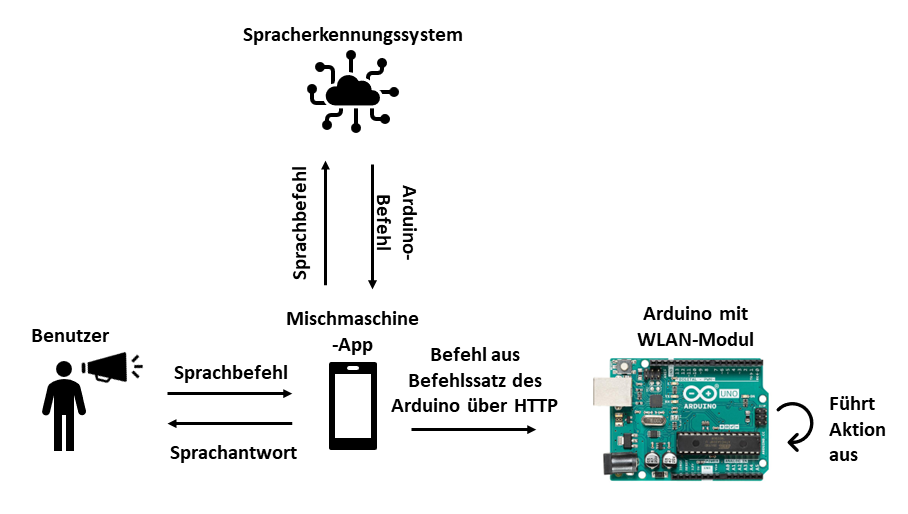
\includegraphics[width=0.8\textwidth]{Bilder_Konzept/Konzept_B.png}}
    \caption{\label{figure:Konzept_mobile_App}Spracherkennung und -verarbeitung mittels mobiler Anwendung}
\end{figure}
\noindent
Ein Problem dieser Lösung ist der offensichtliche Mehraufwand durch die Entwicklung einer eigenen Anwendung für Mobiltelefone.
Auch der Anwender hat zusätzlichen Aufwand durch die Installation.
Außerdem ist die Spracheingabe und -ausgabe über das Mobiltelefon nicht intuitiv, da der Anwender eigentlich mit der Maschine kommunizieren sollte.
Dieser Effekt kann dadurch abgeschwächt werden, dass wenigstens die Antwort durch einen Lautsprecher in der Mischmaschine an den Benutzer zurückgegeben wird.
\section{Konzept C: Spracherkennung und -verarbeitung auf Computer-Hardware}
Ein weiteres Konzept stützt sich auf die Verwendung eines Computers in der Mischmaschine anstelle eines Mikrocontrollers wie dem Arduino.
Motivation ist hierbei der Leistungsgewinn gegenüber eines Mikrocontrollers, um die Spracherkennung und -verarbeitung mittels Sprachmodell zu gewährleisten.
Ein Beispiel für einen solchen Miniaturcomputer ist der Raspberry-Pi.
Dieser bietet genügend Schnittstellen, wie etwa USB-Hubs, zum verbinden von Mikrofon als auch Lautsprecher.
Nimmt der Computer das Audiosignal auf verarbeitet er dieses und generiert daraus die Antwort, die durch den Lautsprecher ausgegeben wird, zusammen mit der Aktion für die Getränkemischmaschine.
Diese muss an den Arduino, welcher die Mischmaschine steuert, übermittelt werden.
Um dies zu ermöglichen können der Computer und der Arduino über eine serielle Schnittstelle, wie etwa einem USB-Kabel, miteinander  verbunden werden.
Abbildung \ref{figure:Konzept_Raspberry} stellt den konzeptionellen Aufbau graphisch dar.
\begin{figure}[H]
    \centering
    \fbox{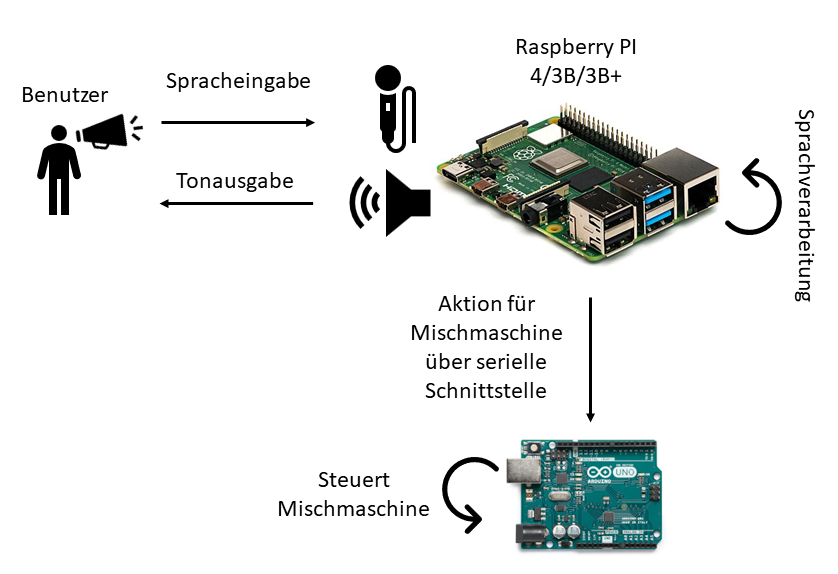
\includegraphics[width=0.8\textwidth]{Bilder_Konzept/Konzept_C.png}}
    \caption{\label{figure:Konzept_Raspberry}Spracherkennung und -verarbeitung auf Computer-Hardware}
\end{figure}
\noindent
Obwohl ein Computer wie der Raspberry-Pi im Allgemeinen eine höhere Leistung als ein Mikrocontroller hat ist damit nicht sichergestellt, dass diese zur Ausführung des Sprachmodells ausreicht.
Beispielsweise ist das vierte Modell der Raspberry-Pi-Serie mit nur maximal acht Gigabyte Arbeitsspeicher erhältlich.
Das Sprachmodell könnte allerdings noch weitaus mehr Daten im Arbeitsspeicher benötigen.
Des Weiteren ist zu beachten, dass die Miniaturcomputer von Raspberry-Pi im Speziellen zum Zeitpunkt dieser Arbeit kaum zu vertretbaren Preisen verfügbar sind.
\section{Finales Hardware-Konzept}
Die folgende Tabelle zeigt eine Übersicht bezüglich der Bewertung der einzelnen Konzepte.
\begin{table}[H]
    \centering
    \begin{tabular}{l|c|c|c|c}
        Bewertungsmatrix          & \makecell{Konzept A                                     \\ (nur Arduino)} & Konzept A & Konzept B & Konzept C \\
        \hline
        \makecell[l]{Freiheitsgrade in der Spracheingabe                                    \\ des Benutzers} & niedrig                    & sehr hoch & sehr hoch & hoch      \\
        \hline
        Hardwarekosten            & niedrig             & hoch      & niedrig   & sehr hoch \\
        \hline
        Verfügbare Rechenleistung & niedrig             & sehr hoch & sehr hoch & hoch      \\
        \hline
        Performanz                & sehr hoch           & mittel    & mittel    & sehr hoch \\
        \hline
        Overhead                  & niedrig             & hoch      & sehr hoch & niedrig   \\
    \end{tabular}
    \caption{\label{table:Bewertungsmatrix_Konzepte}Bewertung der Konzepte}
\end{table}
\noindent
Ein erster Ansatz wurde im Kapitel \ref{section:Konzept_A} zu Konzept A erläutert.
Hierbei war die Idee, die Spracherkennung und -verarbeitung nur auf dem Arduino auszuführen.
Aufgrund der mangelnden Leistung eines Arduinos können mit Hilfe von Sprachmodulen jedoch nur vordefinierte Sätze oder Wörter erkannt werden.
Damit ist der Freiheitsgrad in der Spracheingabe des Benutzers äußerst eingeschränkt.
Dafür sind die aufzuwendenden Hardwarekosten minimal.
Lediglich das Sprachmodul sowie ein Lautsprecher müssten besorgt werden.
Die Performanz wird als sehr hoch eingeschätzt, da die Spracherkennung direkt auf dem Ardunino erfolgen kann, der auch die Mischmaschine steuert.
Niedrig ist hingegen der benötigte Mehraufwand, da kaum zusätzliche Awendungen, Services oder Hardwarekomponenten benötigt werden.\\\\
Das Konzept wurde schließlich durch einen Sprachverarbeitungsservice in der Cloud ergänzt (Konzept A).
Der Benutzer hat bei diesem Ansatz große Freiheiten in seinen Formulierungen, da es kein Problem darstellt ein großes Sprachmodell in der Cloud auszuführen.
Die Hardwarekosten könnten allerdings hoch sein, je nach dem, ob der Server selbst bereitgestellt oder von einem externen Anbieter bezogen wird.
Auch die letzten Endes tatsächlich benötigte Rechenleistung spielt dabei eine Rolle.
Die verfügbare Rechenleistung ist theoretisch unbegrenzt, wobei die Performanz des Gesamtsystems nur als mittelmäßig eingestuft werden kann.
Nach der Aufnahme und eventuell einer Vorverarbeitung des Aduiosignals durch den Arduino müssen \ac{HTTP}-Nachrichten gesendet und Empfangen werden.
Je nach Last auf dem Netzwerk kann es dadurch zu Latenzen oder sogar Verbindungsabbrüchen kommen.
Außerdem ist der Overhead durch den Einsatz einer Cloud recht hoch.\\\\
Konzept B unterscheidet sich in Sachen Freiheitsgrad, Rechenleistung und Performanz nicht von Konzept A, da auch hier eine Cloud zum Einsatz kommt.
Die Hardwarekosten sind jedoch niedriger, da immerhin kein Sprachmodul, Mikrofon und Lautsprecher benötigt werden.
Die Aufgaben dieser Komponenten kann das Mobiltelefon des Anwenders übernehmen.
Der Overhead ist deutlich größer, da das Konzept die Entwicklung einer eigenen Mobilanwendung voraussetzt.\\\\
Der Freiheitsgrad wird bei Konzept C als hoch, jedoch nicht als sehr hoch, bewertet.
Grund hierfür ist die, im Vergleich zur Cloud, etwas beschränkte Leistung, welche die Leistung/Größe des Sprachmodells beeinträchtigen könnte.
Hardwarekosten können jedoch sehr hoch werden.
Bei dem Einsatz einer Cloud kann ein günstiger Anbieter gefunden werden, sodass die Anschaffung eigener Hardware entfällt.
Dies ist hier nicht der Fall.
Die Performanz des Gesamtsystems kann, wie bei Konzept A (nur mittels Arduino), sehr hoch eingeschätzt werden, da Spracherkennung und -verarbeitung direkt in der Mischmaschine von der Hardware übernommen wird.
Der Mehraufwand ist gering, da weder ein Cloudservice noch eine externe Anwendung entwickelt werden müssen.\\\\
Letzten Endes wurde das Konzept C als finales Hardware-Konzept gewählt. Wie ein Blick in die Bewertungsmatrix zeigt lässt sich dies mit den sehr guten Werten, die sich aus der Betrachtung der beschriebenen Bewertungskriterien ergaben, begründen.
\section{Konzept für die Sprachsteuerung}
\subsection{Ansatz für das Dialogsystem}
Aus dem Vergleich der wichtigsten Ansätze zur Erstellung von Chatbots, die in Kapitel \ref{sec:ansaetze_erstellung_chatbots} besprochen wurden, lassen sich die folgenden Vor- und Nachteile der einzelnen Methoden ableiten:
\begin{table}[H]
    \centering
    \begin{tabular}{m{3cm}|m{6cm}|m{6cm}}
        Ansatz               & Vorteile                                                  & Nachteile \\
        \hline
        Musterabgleich       & \makecell[l]{\tabitem Einfacher Einstieg                              \\ \tabitem Leicht wiederverwendbar\\ \tabitem Modularität\\ \tabitem Leicht zu kontrollieren/\\einzuschränken} & \makecell[l]{\tabitem Themenbereich begrenzt\\ \tabitem Die Möglichkeiten sind durch\\ die Arbeitsbelastung des\\ Entwicklers begrenzt\\ \tabitem Komplexität der Fehlersuche\\ \tabitem Strenge und \glqq{}spröde\grqq{} Regeln} \\
        \hline
        Grounding            & \makecell[l]{\tabitem Gut im Beantworten logischer\\ Fragen             \\\tabitem Leicht zu kontrollieren/\\einzuschränken}             & \makecell[l]{\tabitem Künstlicher, mechanischer Ton \\ \tabitem Probleme mit Zweideutigkeiten \\ \tabitem Probleme mit dem Allgemein-\\wissen \\ \tabitem Begrenzt auf strukturierte\\ Daten \\ \tabitem Erfordert die Extraktion von\\ Informationen in großem Umfang \\ \tabitem Erfordert menschliche Aufsicht}    \\
        \hline
        Suche                & \makecell[l]{\tabitem Einfachheit                                     \\ \tabitem Leicht zu lehren \\ \tabitem Simulation von menschlicher\\ Konversation}             & \makecell[l]{\tabitem Unzureichende Skalierung \\ \tabitem Die simulierte Persönlichkeit des\\ Bots ist inkonsistent \\ \tabitem Kennt den Kontext nicht \\ \tabitem Keine sachlichen Fragen} \\
        \hline
        \makecell[l]{Generierungs-\\methoden} & \makecell[l]{\tabitem Neue, kreative Dialoge                          \\ \tabitem Weniger Arbeit für den\\ Entwickler \\ \tabitem Kontextsensitiv}           & \makecell[l]{\tabitem Schwierig zu lehren \\ \tabitem Erfordert mehr Daten (Dialoge) \\ \tabitem Schwierig, in die richtige\\ Richtung zu lenken \\ \tabitem Erfordert mehr Rechenleistung} \\
    \end{tabular}
    \caption{\label{table:Bewertungsmatrix_Konzepte_Dialogsysteme}Bewertung der Ansätze für die Erstellung eines Dialogsystems}
\end{table}
\noindent
Bei der Analyse des Problems, ein Dialogsystem für eine Getränkmischmaschine zu entwickeln, kann man zu dem Schluss kommen, dass die beste Option eine Mischung aus dem Ansatz der Informationssuchemethode und dem Musterabgleich ist.\\\\
Das erste Argument, das für diesen Ansatz spricht, ist die Möglichkeit, die Sprachsteuerung in deutscher Sprache zu verwenden, was die Anwendung der Generierungsmethoden erschwert, da der Zugang zu einer geeigneten Datenbank in dieser Sprache, die den Anforderungen des Projekts, nämlich eine ausreichende Anzahl von Beleidigungen zu enthalten, nicht möglich ist.
Gleichzeitig können bei der Verwendung von Musterabgleich Antwortvorlagen und Muster für entsprechende Anfragen in deutscher Sprache im Voraus erstellt werden, was die Erstellung und das Training des Dialogsystems erleichtert.\\\\
Das zweite Argument ist, dass in diesem Projekt ein Raspberry Pi verwendet wird, was die Verwendung generativer Methoden aufgrund der begrenzten Hardware-Ressourcen einschränken kann.
Andererseits kann das Modell für die Informationssuche und den Musterabgleich auf Geräten mit geringem Stromverbrauch implementiert werden, was diesen Ansatz für dieses Projekt vorteilhaft macht.\\\\
Generierungsmethoden könnten auch für dieses Problem zu mächtig sein.
Beim Mixen von Cocktails können die Antworten einfach und formelhaft sein, wie z. B. \glqq{}Das hört sich eklig an, bist du sicher, dass du es willst?\grqq{} oder \glqq{}Ich hoffe, ich sehe dich nie wieder\grqq{}.
In diesem Fall kann der Einsatz von Generierungsmethoden wie seq2seq-Modellen überflüssig und ineffizient sein.
Für diese Aufgabe ist im Gegensatz zu komplexen natürlichsprachlichen Abfragen keine detaillierte semantische Verarbeitung erforderlich, so dass der Musterabgleich einen einfacheren und effizienteren Ansatz darstellt.\\\\
Bei der Verwendung des Musterabgleiches kann man den Ton und den Humor des Geräts leicht steuern und so die gewünschte Atmosphäre erzeugen.
Die Antworten des seq2seq-Modells sind wiederum sehr schwer zu steuern.
Generierungsmethoden können zu unerwünschtem Maschinenverhalten führen, wenn das Modell auf ungeeigneten Daten trainiert wird oder Fehler in der Betriebslogik enthält.
Die Verwendung einer Datenbank, die genügend Beleidigungen enthält (z. B. die 4chan-Datenbank), kann dazu führen, dass die Antworten der Maschine über das Ziel hinausschießen und statt lustig zu sein, den Benutzer beleidigen.\\\\
Mit diesem Ansatz wird auch die Effizienz der Maschinensteuerung verbessert.
Beim Musterabgleich kann eine Kategorie \glqq{}Getränkebestellung\grqq{} zugewiesen werden, die, wenn sie erkannt wird, die Maschine automatisch zur Bearbeitung der Befehle veranlasst.
Im Falle von seq2seq-Modell ist keine Kategorie vorgesehen, so dass eine zusätzliche Prüfung jeder Eingabeanweisung eingeführt werden müsste, um festzustellen, wann der Benutzer die Bestellung aufgegeben hat.\\\\
Ein letztes Argument, das für den Ansatz spricht, ist die Möglichkeit, die Maschine bei Bedarf schnell an neue Anfragen und Anforderungen anzupassen, indem neue Muster und Regeln in das System eingeführt werden.
Daher ist eine Mischung aus Informationssuchemethode und Musterabgleich für das vorliegende Problem am besten geeignet.
\subsection{Befehle}
Folgende Übergangsdiagram beschreibt die Abfolge von Aktionen und Übergängen zwischen Zuständen bei der Analyse der Befehle:
\begin{figure}[H]
    \centering
    \fbox{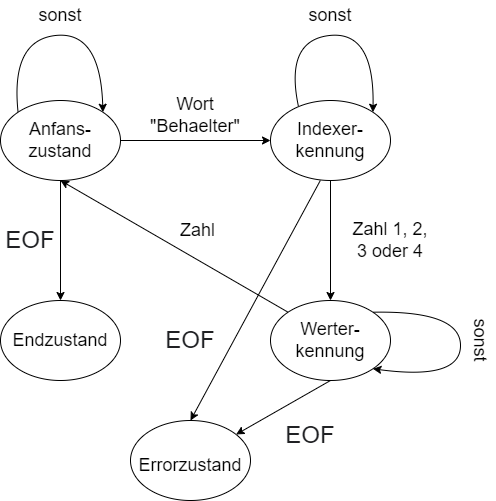
\includegraphics[width=0.8\textwidth]{Bilder_Konzept/uebergangsdiagram.png}}
    \caption{\label{figure:Uebergangsdiagram_Befehle}Übergangsdiagram beim Analyse der Befehle}
\end{figure}
\noindent
In diesem Fall erhält die Methode eine Zeichenkette mit Informationen über den prozentualen Anteil von Flüssigkeiten aus verschiedenen Behälter und muss den prozentualen Anteil jeder Flüssigkeit zurückgeben.\\\\
Der erste Zustand \glqq{}Anfangszustand\grqq{} bedeutet, dass die Methode gestartet wird. Dann verarbeitet die Methode nacheinander jedes Wort der Eingabezeichenkette. 
Jedes Eingabewort, außer Wort \glqq{}Behälter\grqq{} wird als irrelevant wahrgenommen und erstmal ignoriert.\\\\ 
Sobald die Maschine das Wort \glqq{}Behälter\grqq{} hört, geht die Methode zum nächsten Zustand über - der Indexerkennung. 
Nach den Regeln kommt der Index nach dem Wort \glqq{}Behälter\grqq{}, aber zwischen dem Wort \glqq{}Behälter\grqq{} und der Indexzahl können andere Wörter stehen, die für diese Methode nicht relevant sind, z. B. \glqq{}Nummer\grqq{} oder \glqq{}mit Nummer\grqq{}. 
Daher werden diese Wörter ignoriert, und die Maschine bleibt in demselben Zustand, bis sie eine Zahl zwischen eins und vier hört.\\\\
Sobald der Index ermittelt ist, geht die Methode zum nächsten Zustand über - der Wertrmittlung. 
In diesem Fall werden die Wörter, angefangen mit dem Wort \glqq{}Behälter\grqq{}, in umgekehrter Reihenfolge betrachtet, da der Wert nach den Regeln der Grammatik vor dem Wort \glqq{}Behälter\grqq{} stehen wird. 
Alle Wörter bis zur ersten gefundenen Zahl werden ignoriert. 
Sobald die Maschine eine beliebige Zahl hört, kehrt die Methode in den Ausgangszustand zurück.\\\\
Die Analyse der Befehle kann dann zum Endzustand kehren, wenn sie aktuell sich im Anfangszustand befindet und alle Wörter gelesen wurden. 
Sobald die Zeichenkette in einem anderen Zustand beendet wird, wird die Methode zum Errorzustand kehren.
\endinput




\chapter{Implementierung}
\section{Implementierung des Sprachverarbeitungssystems}\label{section:Implementierung_Sprachverarbeitung}
\subsection{Word2Vec-Modell}
\subsection{Sequence-to-Sequence-Modell}
\section{Implementierung der Sprachsteuerung}
Im Folgenden wird erläutert, wie die Sprachsteuerung für die Getränkemischmaschine implementiert wurde und welche Technologien dafür zum Einsatz kamen. Dabei wird zunächst auf die Spracherkennung d.h., die Umwandlung der Audiosignale (Sprachbefehl des Benutzers) in eine Form, die innerhalb des Quelltextes weiterverarbeitet werden kann, eingegangen (s. Abschnitt \ref{section:Spracherkennung}). Danach wird die Anbindung des Sprachverarbeitungssystems beschrieben, dessen Implementierung in Abschnitt \ref{section:Implementierung_Sprachverarbeitung} erklärt wird. Abschließend wird die Kommunikation mit der Mischmaschine über den Arduino illustriert (s. Abschnitt \ref{section:Befehlsverarbeitung}).
\subsection{Spracherkennung}\label{section:Spracherkennung}
Die Spracherkennung ist der erste Schritt bei der Implementierung einer Sprachsteuerung für die Getränkemischmaschine. Mit Spracherkennung ist die Aufnahme eines Tonsignals über ein Audio-Eingabegerät (Mikrofon) und die Umwandlung der Audiodaten in Text gemeint. Der Quelltext zur Implementierung der Sprachsteuerung erfolgt mit der Programmiersprache \textit{Python}, da hier sehr viele, leicht zu bedienende Bibliotheken zur Spracherkennung, -verarbeitung und \ac{KI} zur Verfügung stehen.\\\\
Für dieses Projekt viel die Wahl auf das Paket \textit{SpeechRecognition}, das die Verwendung verschiedener Spracherkennungsdienste über eine einheitliche Schnittstelle ermöglicht und zu diesem Zweck auch zur Aufnahme und Verarbeitung der Audiosignale verwendet werden kann \cite{speechrecognition}. Ein großer Vorteil davon ist, dass dadurch ein schneller Wechsel der eingesetzten \ac{API} erfolgen kann, sollte dies erforderlich sein. Die Verwendung des \textit{SpeechRecognition}-Pakets findet fast ausschließlich über die \textit{Recognizer}-Klasse statt. Um Audiosignale über eine physische Audioquelle (bspw. ein Mikrofon am Computer) aufzunehmen kann die \textit{Microphone}-Klasse verwendet werden, die ebenfalls im Paket enthalten ist. Mit Hilfe eines Objekts vom Typ \textit{Microphone} und der Methode \textit{listen} der \textit{Recognizer}-Klasse können anschließend Audiodaten aufgenommen werden, die in einem Objekt vom Typ \textit{AudioData} gespeichert sind. Die Verwendung von \textit{Recognizer} und \textit{Microphone} sind in Listing \ref{speech_rec_1} zu sehen. 
\lstinputlisting[language=python, style=algoBericht, label={speech_rec_1}, basicstyle=\tiny\sffamily, captionpos=b, caption={Audioaufnahme mit \textit{SpeechRecognition}}]{./Listings/speech_rec_1.py}
Das \textit{AudioData}-Objekt kann nun verwendet werden um die darin gespeicherten Audiodaten zu erkennen und in Text umzuwandeln. Das \textit{SpeechRecognition}-Paket stellt dafür verschiedene Möglichkeiten zur Verfügung, wie eingangs erwähnt wurde. Diese sollen im Folgenden kurz beschrieben werden:
\begin{itemize}
    \item Whisper: Whisper ist ein neuronales Netz das von der Firma \textit{OpenAI} trainiert und als Open-Source-Projekt zur Verfügung gestellt wird \cite{openai,whisper}. Neben der Fähigkeit Sprache in Text zu konvertieren kann es auch eingesetzt werden um Transkripte zu generieren, die gesprochene Sprache automatisch zu erkennen oder in die englische Sprache zu übersetzen. Das Paket \textit{SpeechRecognition} lässt sowohl die Verwendung der von \textit{OpenAI} zur Verfügung gestellten Online-\ac{API} zu, als auch die lokale Ausführung des Sprachmodells. Aufgrund der Anforderung nach Offline-Funktionalität entfällt die erste Möglichkeit (s. Kapitel \ref{chap:Anforderungen}).
    \item Sphinx: Das \textit{CMUSphinx} Projekt wird von der \ac{CMU} unterhalten und stellt eine Reihe von Werkzeugen und Bibliotheken zur Spracherkennung zur Verfügung \cite{sphinx_about}. Darunter fallen bspw. \textit{PocketSphinx}, \textit{SphinxTrain} und \textit{sphinx4}. Bei \textit{PocketSphinx} handelt es sich um eine C-Bibliothek zur Spracherkennung, die auch innerhalb von Python verwendet werden kann. \textit{SphinxTrain} hingegen stellt Ressourcen zum Trainieren eigener Modelle bereit. \textit{sphinx4} ist das Java-Equivalent zu \textit{PocketSphinx}. Somit ist für dieses Projekt nur \textit{PocketSphinx} interessant. Leider unterstützt enthält das Paket standardmäßig nur ein Modell für die englische Sprache. Anderssprachige Modelle und weitere dazugehörige Ressourcen müssen mühsam aus externen Quellen bezogen und eingebunden werden.
    \item Snowboy: \textit{Snowboy Hotword Detection} ist ein quelloffenes Projekt welches Bibliotheken für verschiedene Programmiersprachen bereitstellt, die dem Erkennen sog. \glqq{}hot words\grqq{} dienen \cite{snowboy}. Ein \textit{hot word} sind ein oder mehrere Wörter die der Aktivierung eines Sprachsteuerungssystems dienen. Bekannte Beispiele hierfür sind \glqq{}Alexa\grqq{} oder \glqq{}OK Google\grqq{}. Das System \glqq{}hört\grqq{} im Hintergrund und wartet darauf, dass das \textit{hot word} genannt wird. Anschließend nimmt das System weitere Sätze, die vom Benutzer gesprochen werden, wahr und verarbeitet diese. Ein \textit{hot word} ist notwendig damit das System nicht dauerhaft versucht Sätze zu verarbeiten, die nicht für das System gedacht sind und damit wiederholt Fehler bekommt oder unerwünschtes Verhalten an den Tag legt. Da die Ansprüche des vorliegenden Projekts an die Detektion von \textit{hot words} nicht besonders hoch sind und um die von Snowboy benötigte Rechenzeit einzusparen wird \textit{Snowboy} in diesem Projekt keine Relevanz haben. Auf die konkrete Umsetzung des \textit{hot word} Mechanismus wird später noch eingegangen. Ein weiterer Grund dafür, dass Snowboy nicht zum Einsatz kommen soll ist, dass das Projekt bereits im Jahr 2020 offiziell eingestellt wurde und nur noch von der Community weiter betrieben wird. 
    \item Vosk: Das \textit{Vosk Speech Recognition Toolkit} ist neben \textit{Whisper} und \textit{Sphinx} die dritte und letzte verfügbare offline \ac{API} für die \textit{SpeechRecognition} eine Schnittstelle bereitstellt \cite{vosk,vosk_repo}. Es wird von der \textit{Alpha Cephei Incorporation} vertrieben. Ähnlich wie bei Whisper sind vortrainierte Modelle in vielen verschiedenen Sprachen bereits vorhanden, müssen allerdings manuell heruntergeladen und dem \textit{SpeechRecognition} Paket zur Verfügung gestellt werden.
    \item Google: \textit{SpeechRecognition} bietet zwei Möglichkeiten Google-Dienste zur Konvertierung von Sprache zu Text zu verwenden. Die erste Möglichkeit besteht in der Verwendung der \textit{Google Speech API} in der \textit{Google Cloud} \cite{google_cloud_speech}. Die zweite Möglichkeit besteht in der Verwendung der \textit{Google Speech API} ohne die \textit{Google Cloud}. Die Verwendung der Google-Schnittstelle entfällt jedoch für dieses Projekt, da eine aktive Internetverbindung Voraussetzung dafür ist. Außerdem sind die Google-Dienste weder kostenfrei noch open-source.
    \item Microsoft: Auch hier gibt es zwei verschiedene Möglichkeiten Microsoft-Dienste zur Umwandlung von Sprache zu Text über das \textit{SpeechRecognition}-Paket zu nutzen. Eine davon ist die Verwendung der \textit{Speech to text} Funktion in der \textit{Microsoft Azure Cloud} \cite{azure_speech_to_text}. Hierfür sind ein aktiver \textit{Azure}-Account sowie ein gültiger \ac{API}-Schlüssel notwendig. Die zweite Möglichkeit besteht in der \textit{Microsoft Bing Voice Recognition}. Diese ist jedoch veraltet und wird nicht mehr unterstützt. Auch diese Schnittstelle enfällt jedoch wegen der notwendigen Internetverbindung und Bezahlung. 
    \item IBM: Auch die Firma IBM bietet ihre eigene Schnittstelle zur Spracherkennung mit Hilfe der von IBM entwickelten \ac{KI} \textit{Watson} an \cite{ibm_speech_to_text}. Auch hier gilt: zur Verwendung der \ac{API} ist sowohl eine aktive Internetverbindung als auch Bezahlung vorgesehen, weshalb diese Schnittstelle für das Projekt nicht in Frage kommt.
    \item Weitere Schnittstellen sind \textit{Wit.ai}, \textit{Houndify} und \textit{Tensorflow} \cite{witai,houndify,tensorflow_home}. Da diese Schnittstellen allderdings ebenso eine aktive Internetverbindung voraussetzen und damit ausscheiden soll nicht weiter auf sie eingegangen werden.
\end{itemize}
Die einzelnen \ac{API}s lassen sich jeweils über einen Methodenaufruf der Form \textit{Recognizer.recognize\_x} verwenden, wobei das \glqq{}x\grqq{} für den Namen der jeweiligen \ac{API} steht. Für dieses Projekt viel die Wahl auf die Verwendung der \textit{Whisper}-Bibliothek von \textit{OpenAI}. Dies ist damit zu begründen, dass sie von den offline verwendbaren \ac{API}s die mit Abstand am einfachsten zu verwendende ist und gleichzeitig sehr gute Ergebnisse beim Testen damit erzielt wurden. Beispielsweise werden die Modelle für viele verschiedene Sprachen bereits von OpenAI zur Verfügung gestellt und für jedes Modell stehen weitere Ausführungen zur Verfügung die nach den eigenen Ansprüchen und vorhandenen Ressourcen ausgewählt werden können. Die verschiedenen Ausführungen sind nach der \glqq{}Größe\grqq{} des Modells unterteilt in \glqq{}tiny\grqq{}, \glqq{}base\grqq{}, \glqq{}small\grqq{}, \glqq{}medium\grqq{} und \glqq{}large\grqq{} \cite{whisper_repo}.
\lstinputlisting[language=python, style=algoBericht, label={speech_rec_2}, basicstyle=\tiny\sffamily, captionpos=b, caption={Sprache zu Text mit \textit{OpenAI Whisper}}]{./Listings/speech_rec_2.py}
Listing \ref{speech_rec_2} zeigt, wie mit Hilfe der \textit{Whisper}-\ac{API} die aufgenommenen Audiodaten zu Text verarbeitet und ausgegeben werden können. Die Sprache und die Modellgröße werden bei dem Methodenaufruf \textit{Recognizer.recognize\_whisper} angegeben. Sollte das entsprechende Modell noch nicht lokal vorliegen wird dieses bei der ersten Ausführung automatisch installiert, was einen hohen Grad an Benutzerfreundlichkeit seitens der \ac{API} bedeutet. 
\subsubsection{Herausforderungen bei der Implementierung der Spracherkennung}
Die Verwendung von \textit{Whisper} setzt die Installation von \textit{PyTorch} voraus - einem quelloffenen \ac{ML}-Framework \cite{pytorch}. Die Installation von \textit{PyTorch} kann auf zwei unterschiedlichen Wegen erfolgen:
\begin{enumerate}
    \item Unter der Benutzung vorkompilierter Distributionen mit Hilfe eines Paketverwaltungssystems wie etwa \textit{pip} \cite{pip}.
    \item Durch das eigenständige Bauen des Quelltextes auf dem lokalen Rechner.
\end{enumerate}
Da es sich bei \textit{PyTorch} um ein überaus großes und komplexes Projekt handelt ist es empfehlenswert die erste Methode anzuwenden, da der Build-Vorgang bei Methode zwei sehr viele Ressourcen benötigt.\\\\
Nach der Verwendung von \textit{pip} zur Installation von \textit{PyTorch} auf dem für das Projekt verwendeten \textit{Raspberry Pi 4B} kam es jedoch zu einem unerwarteten Fehler. Das Importieren der \textit{PyTorch}-Bibliothek ließ das Programm sofort beenden und die Nachricht \glqq{}Illegal Instruction\grqq{} auf dem Bildschirm ausgeben. Die Fehlermeldung lässt darauf schließen, dass die Bibliothek einen für den Prozessortyp unbekannten Befehl ausüben will. Drei Lösungsansätze wurden daraufhin konzipiert:
\begin{enumerate}
    \item Das Programm sollte mit einer anderen Python-Version ausgeführt werden.
    \item Das vorkompilierte Paket, das automatisch von \textit{pip} ausgewählt wurde scheint nicht auf die vorhandene Prozessorarchitektur zu passen und führt unbekannte Maschinenbefehle aus. Deshalb sollte die \textit{PyTorch}-Bibliothek selbstständig, lokal kompiliert werden.
    \item Ein anderes vorkompiliertes Paket herunterladen und installieren, das auf die vorhandene Prozessorarchitektur angepasst und optimiert ist.
    \item Sollten alle zuvor genannten Versuche scheitern muss \textit{Whisper} durch eine andere Bibliothek ersetzt werden, die keine Abhängigkeit zu \textit{PyTorch} aufweist.
\end{enumerate}
Lösungsansatz eins erwies sich als nicht effektiv. Das Programm verursachte immernoch den selben Fehler. Lösungsansatz zwei scheiterte, da der Build-Prozess mehr als den zur Verfügung stehenden \ac{RAM} des Raspberry Pi aufbrauchte. Sogar mit vier \ac{GB} zusätzlich konfiguriertem Swap-Speicher wurde der Build-Prozess nach einiger Zeit vom Betriebssystem beendet aufgrund des hohen \ac{RAM}-Verbrauchs. Lösungsansatz drei funktionierte schließlich. Mit Hilfe des vorkompilierten Pakets aus \cite{q-engineering_install_nodate} konnte \textit{PyTorch} installiert und erfolgreich importiert und verwendet werden.\\\\
Ein weiteres Problem trat bei der Verwendung des Mikrofons über die \textit{SpeechRecognition}-Bibliothek auf. Bei den Aufrufen \textit{speech\_recognition.Microphone()} und\\ \textit{speech\_recognition.Recognizer().listen(source)} kommt es auf dem Raspberry Pi zu unerwarteten Fehlermeldungen, die in Abbildung \ref{img:alsa_errors} zu sehen sind.
\begin{figure}[H]
    \centering
    \fbox{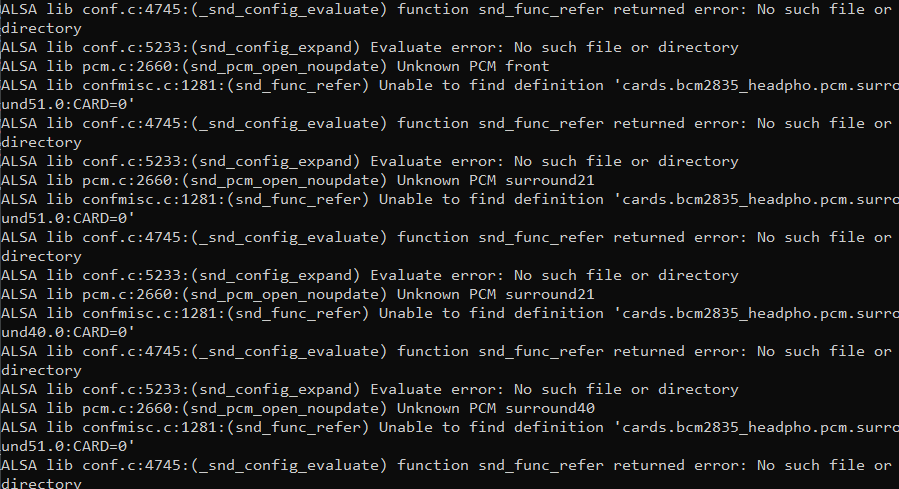
\includegraphics[width=0.8\textwidth]{./img/Bilder_Implementierung/alsa_errors.png}}
    \caption{Fehlermeldungen beim Zugriff auf das Mikrofon}
    \label{img:alsa_errors}
\end{figure}
\noindent
Zwar kann das Programm trotz der Meldungen fehlerfrei ausgeführt werden, jedoch stören die Meldungen bspw. beim Debuggen und irritieren evtl. Programmierer, die zu einem späteren Zeitpunkt einen Blick auf das Projekt werfen. Um die Fehlermeldungen zu umgehen wurde deshalb im finalen Quelltext die Fehlerbehandlungsfunktion der \textit{libasound}-Bibliothek ausgetauscht wie in Listing \ref{speech_rec_3} zu sehen ist.
\lstinputlisting[language=python, style=algoBericht, label={speech_rec_3}, basicstyle=\tiny\sffamily, captionpos=b, caption={Fehlerbehandlung}]{./Listings/speech_rec_3.py}
Für einen Vorher-/Nachher-Vergleich sei auf Listing \ref{speech_rec_2} verwiesen. Zeilen vier bis zehn dienen der Definition einer C-Funktion zur Fehlerbehandlung, die bei ihrer Ausführung die auftretende Meldung ignoriert. In Zeile 16 wird die Standard Fehlerfunktion durch diese ersetzt und in Zeile 19 wieder zurückgeändert. 
\subsection{Anbindung des Sprachmodells an die Mischmaschine}
\subsection{Befehlsverarbeitung in der Mischmaschine}\label{section:Befehlsverarbeitung}
Nachdem die Sprache des Benutzers erkannt, in Text konvertiert und durch das Sprachmodell interpretiert wurde muss der zurückerhaltene Befehl vom Raspberry Pi and den Arduino in der Getränkemischmaschine gesendet werden. Zur Umsetzung der Kommunikation zwischen Raspberry Pi und Arduino kommt die \textit{PySerial}-Bibliothek zum Einsatz \cite{pyserial}. Listing \ref{serial_1_py} zeigt, wie die Bibliothek zum Versenden von Nachrichten an ein Gerät über die serielle Schnittstelle erfolgen kann.
\lstinputlisting[language=python, style=algoBericht, label={serial_1_py}, basicstyle=\tiny\sffamily, captionpos=b, caption={Serielle Kommunikation in Python}]{./Listings/serial_1.py}
Das Programm öffnet in Zeile vier die serielle Schnittstelle zu dem Gerät mit dem Namen \glqq{}ttyACM0\grqq{}, mit einer Baud-Rate von 9600 und einem Timeout von fünf Sekunden. Der Gerätename ist je nach Gerät und Betriebssystem unterschiedlich und muss zuvor mit den verfügbaren Betriebssystemmitteln bestimmt werden. Die Baud-Rate gibt an, mit welcher Geschwindigkeit Symbole über die Schnittstelle gesendet werden. Die Baud-Rate muss sowohl beim Sender als auch beim Empfänger gleich sein, da es sonst zu Kommunikationsproblemen kommt. Der Timeout steuert wie lange bei einer Leseoperation gewartet werden soll, bis alle zu lesenden Bytes im Puffer vorhanden sind.\\\\
In der darauffolgenden Zeile wird der Eingabepuffer geleert, um zu verhindern, dass unvollständige Daten an den Empfänger gesendet werden, die beim letzten Programmdurchlauf im Puffer verblieben sein könnten. Da der Verbindungsaufbau mit dem Gerät einige Zeit dauern kann wird die Programmausührung in Zeile sechs zunächst um fünf Sekunden verzögert.\\\\
In Listing \ref{serial_1_ino} ist der Quelltext auf Empfängerseite zu sehen.
\lstinputlisting[language=c++, style=algoBericht, label={serial_1_ino}, basicstyle=\tiny\sffamily, captionpos=b, caption={Serielle Kommunikation in Python}]{./Listings/serial_1.ino}
\subsubsection{Herausforderungen bei der Implementierung der Befehlsverarbeitung}
\endinput



\chapter{Fazit und Ausblick}
Im Zuge dieser Arbeit wurde eine Sprachsteuerung für eine Getränkemischmaschine implementiert, mit deren Hilfe der Benutzer Getränke aus den fünf verfügbaren Behältern mischen kann, indem er die Behälter mit der jeweils gewünschten Prozentangabe nennt. Dafür wurde ein Sprachmodell trainiert, welches anhand eines Textes (Spracheingabe des Benutzers) die Prozentangaben für die jeweiligen Behälter extrahiert und die Art der Eingabe klassifiziert. Der Text kann in eine der drei Klassen eingeordnet werden: Bestellung, Begrüßung, Verabschiedung und keine Eingabe. Je nach Klasse werden bestimmte Antworten ausgewählt, die über Lautsprecher an den Benutzer zurückgegeben werden, damit der Eindruck eines Dialogs zwischen Benutzer und Mischmaschine entsteht. Der Code für die Sprachsteuerung wurde in Python implementiert und wird auf einem Raspberry Pi ausgeführt, der an die bestehende Hardware in der Mischmaschine angeknüpft werden musste.
\section{Erfüllung der Anforderungen}
Am Anfang des Projekts wurden verschiedene Anforderungen an das zu entwickelnde System definiert, die nun einer Überprüfung unterzogen werden sollen.\\\\
Um die Anforderung an die Antwortzeit zu testen wurde die Python-Methode \textit{time()} aus der \textit{time}-Bibliothek verwendet, welche die aktuelle Systemzeit zurückgibt. Dafür wurde in Zeile \ref{code:start_time} des Hauptprogramms aus Anhang \ref{Anhang_B} die Startzeit und in Zeile \ref{code:end_time} die Endzeit gemessen und die Differenz als Antwortzeit berechnet. Der Test wurde zehn mal durchgeführt und es ergab sich hierbei eine mittlere Antwortzeit von 26.66 Sekunden, was deutlich über den gewünschten sechs Sekunden liegt. Besonders Zeitaufwendig sind hierbei die Konvertierung der Audiodaten in Text, die Berechnungen des Sprachmodells bei dem Aufruf von \textit{language\_model.get\_response(text)} als auch die Ausgabe der Antwort über die Lautsprecher, die bei den Tests mit eingeflossen ist und deren Dauer von der ausgewählten Antwort abhängt. Dabei beträgt die Ausführungszeit des Sprachmodells etwas über fünf Sekunden. Als Beispielsatz wurde \glqq{}Mischmaschine. Ich hätte gerne ein Getränk zu 50 Prozent aus Behälter 1 und zu 50 Prozent aus Behälter 2.\grqq{} verwendet. Die Ausführungszeit der Spracherkennung liegt bei etwa 15 Sekunden und macht damit den mit Abstand größten Zeitverlust aus.\\\\
Eine weitere Anforderung war, dass zum Betreiben der Mischmaschine zusammen mit der Sprachsteuerung keine Anbindung zum Internet notwendig sein darf. Diese Anforderung wurde formuliert, damit die Mischmaschine an möglichst vielen Orten betrieben werden kann. Sie wurde in der finalen Umsetzung erreicht, indem alles was für die Sprachsteuerung notwendig ist auf lokaler Hardware ausgeführt wird und auf die Auslagerung von Berechnungen auf Cloud-Services o.ä. verzichtet wurde.\\\\
Lautstärke...\\\\
Entfernung...\\\\
Die Antworten der Mischmaschine sollten humorvoll und kontrollierbar sein und die Kommunikation sollte auf Deutsch stattfinden können. Alle diese Anforderungen wurden im finalen Produkt erreicht. Bei dem gewählten Ansatz für das Sprachmodell werden vordefinierte Antworten je Klasse ausgewählt. Dadurch ist die Grenze bzgl. dem Humor nur durch die eigene Kreativität gesetzt und die Kontrollierbarkeit ist trivialerweise gegeben, da die Antworten eben manuell vorgegeben werden und somit klar ist, was die Mischmaschine in einer bestimmten Situation antworten kann und was nicht. Spracherkennung und -verarbeitung sind auf die deutsche Sprache ausgerichtet.\\\\
Kosten...\\\\
Der Speicherplatz der 32 \ac{GB} SD-Karte, die für dieses Projekt zur Verfügung stand wurde nicht ausgelastet. Ebenso konnte das Programm für die Spracherkennung ohne Probleme mit den verfügbaren 4 \ac{GB} Arbeitsspeicher ausgeführt werden. Deshalb gelten die anfangs festgelegten Ziele bzgl. des Arbeits- und Festplattenspeicherverbrauchs als erfüllt. Tatsächlich beläuft sich der noch Verfügbare Speicher im Wurzelverzeichnis des Dateisystems am Ende des Projekts noch auf 18 \ac{GB}, was einer Auslastung von lediglich 37 Prozent entspricht, obwohl betriebssystemseitige Programme und Dateien ebenfalls mit in diese Statistik eingehen. Während die Quellcodedateien dieses Projekts kaum einen nennenswerten Beitrag zu der Gesamtgröße leisten, verbrauchen die Spracherkennungs- und verarbeitungsmodelle hingegen vergleichsweise viel Speicher. Die Größe des \glqq{}tiny\grqq{}-Modells von \textit{OpenAI Whisper} beläuft sich auf 73.801 Kilobyte (die \glqq{}medium\grqq{}-Variante erreicht bereits eine Größe von ungefähr 1.5 \ac{GB}). Die von der \ac{NLTK}-Bibliothek verwendeten Dateien nehmen 60 Megabyte Speicher ein. Der Arbeitsspeicherverbrauch bei der Ausführung der Sprachsteuerung erreicht Spitzen von fast einem Gigabyte, also ein Viertel des verfügbaren Arbeitsspeichers. Getestet wurde der Abreitsspeicherverbrauch mit den Python-Bibliotheken `os' und `psutil'. Der Aufruf \textit{psutil.Process(os.getpid()).memory\_info().rss / 1024 ** 2} ergibt dann den aktuellen Verbrauch in Mebibytes.\\\\
Zu guter letzt sollte das System leicht an neue Begebenheiten angepasst werden können. Als Beispiel wurde das Hinzukommen eines neuen Behälters angeführt. In diesem Fall müsste auf Seiten des Arduinos lediglich ein zusätzlicher Prozentwert ausgelesen und damit die Pumpe für den neuen Behälter angesteuert werden. Für das Sprachmodell ergeben sich keine Änderungen (bis auf die Vergrößerung des Arrays für das Speichern der Prozentwerte), da hier bereits eine beliebige Anzahl von Behältern und Prozentwerten extrahiert werden können. Alles in allem ist das Hinzukommen eines neuen Behälters also mit moderatem Aufwand zu bewerkstelligen. Weitere Änderungen die in Zukunft auftreten könnten sind das Ändern der Sprache oder das Hinzufügen neuer Antworten oder Klassen. All dies ist ebenfalls mit moderatem Aufwand zu handhaben. Zum Hinzufügen neuer Antworten reicht das Abändern der \textit{patterns.json}-Datei. Für eine neue Klasse müssten zunächst Muster, also Beispieltexte, für diese Klasse geschrieben und dann das Modell neu trainiert werden. Beim Ändern der Sprache kann für die Spracherkennung eines der Modelle von \textit{OpenAI Whisper} verwendet werden. Die tatsächlichen Änderungen am Code würden sich auf eine einzige Zeile beim Aufruf der \textit{recognize\_whisper}-Methode von der \textit{SpeechRecognition}-Bibliothek beschränken. Das Sprachmodell zur Klassifizierung und Extraktion müsste jedoch neu trainiert werden.
\section{Probleme}
Ein Problem ist die lange Reaktions- bzw. Antwortzeit des Systems, die im Schnitt bei 26.66 Sekunden liegt. Beim Testen entpuppte sich dabei die Spracherkennung mit dem Modell von \textit{OpenAI Whisper} als größter Zeitfresser und das obwohl bereits das kleinste Modell \glqq{}tiny\grqq{} verwendet wurde.\\\\
Als ein weiteres Problem kann die unintuitive Formulierung der Sprachbefehle, die vom Benutzer gefordert wird, angesehen werden. Die Beschreibung des gewünschten Mischgetränks durch Nennung der einzelnen Behälter und ihrer Prozentangaben könnte von einigen Benutzern als umständlich erarchtet werden (\glqq{}Ich hätte gerne ein Getränk, das zu 50 Prozent aus Behälter 1 und zu 50 Prozent aus Behälter 2 besteht.\grqq{} usw.). Eine intuitivere Formulierung ist bspw. \glqq{}Mischmaschine, bitte gebe mir Getränk xyz aus.\grqq{}. Dazu müsste es die Möglichkeit geben, vordefinierte Mischungen als Getränke in der Mischmaschine abzuspeichern.\\\\
Hardware nicht richtig eingebaut...\\\\
Die Erkennung des Hot-Words \glqq{}Mischmaschine\grqq{} kann verbessert werden. Wenn das Wort \glqq{}Mischmaschine\grqq{} am Anfang des Satzes des Benutzers nicht erkannt wird, dann ist das für den Anwender sehr frustrierend, da er seine Eingabe wiederholen muss. In einem Test mit zehn Versuchen ergab sich, dass das Hot-Word nur in fünf Fällen erkannt wurde. Jedoch hängt die Qualität der Spracherkennung von vielen Faktoren ab, sodass ein Test, der unter anderen Bedingungen stattfindet, evtl. völlig andere Ergebnisse liefern wird. Beispiele für solche Faktoren sind das verwendete Mikrofon und dessen Einstellungen, die Aussprache und Stimmlage des Benutzers, sowie Umgebungsgeräusche. In dem hier dargestellten Test befand sich die Mischmaschine in einem stillen Raum und es wurde auf deutliche und laute Aussprache geachtet.
\section{Mögliche Erweiterungen}
Eine mögliche Erweiterung ist die Verkürzung der Reaktionszeit bei der Spracherkennung. Dies könnte durch die Verwendung einer anderen Spracherkennungs-\ac{API} bzw. eines anderen Modells erreicht werden. Falls keine Bibliothek existiert, die die Anforderungen an die Antwortzeit erfüllt, kann ein eigenes Modell trainiert werden. Dieses könnte so angepasst sein, dass es nur auf eine kleine Teilmenge der deutschen Sprache trainiert ist. Es kommen bei der Anwendung der Sprachsteuerung nämlich nur ein Bruchteil der Worte der deutschen Sprache vor, wie etwa \glqq{}Behälter\grqq{}, \glqq{}Mischmaschine\grqq{}, \glqq{}Getränk\grqq{} oder Zahlen. Dadurch kann das Modell klein und performant gehalten werden. Auch sollte die Spracherkennung insgesamt dadurch verbessert werden, da nicht so viele Worte existieren, zwischen denen unterschieden werden muss.\\\\
Das Speichern vordefinierter Mischungen in Form von Getränken in der Mischmaschine ist eine weitere sinnvolle Ergänzung. Dies kann sinnvollerweise in der bereits existierenden Administrationsansicht der Getränkemischmaschine über das Touch-Display erfolgen. Die Daten über die Getränkekonfigurationen könnten dabei an den Raspberry Pi übertragen werden, der diese persistiert. Das Sprachmodell müsste auf eine Art und Weise angepasst werden, die es ermöglicht, Getränkenamen aus dem Text zu extrahieren. Die Mischungsverhältnisse, die dem Namen zugeordnet sind könnten dann wieder zur Ansteuerung der Pumpen verwendet werden.\\\\
Im Moment dient die Sprachsteuerung lediglich der Bestellung von Getränken. In Zukunft ist es jedoch denkbar den Umfang der verfügbaren Befehle auszuweiten. Als sinnvoll erachtete Befehle sind bspw. die Administration der Mischmaschine über die Sprachsteuerung, das Einleiten des Spülvorgangs, das Umbenennen von Behältern oder das Anlegen von Getränkekonfigurationen.\\\\
Um unnötige Hardware aus der Mischmaschine zu entfernen kann in Betracht gezogen werden den Arduino-Mikrocontroller vollständig durch den Raspberry Pi zu ersetzen und dafür die \ac{GPIO}-Pins des Raspberry zu verwenden, die kurz in Abschnitt \ref{section:raspberry} beschrieben wurden. Die beiden Pins GPIO 14 (TXD) und GPIO 15 (RXD), sowie einer der Ground-Pins können für die serielle Kommunikation mit dem \textit{Nextion}-Display verwendet werden. Fünf weitere Pins für das Steuern der Pumpen (alle \ac{GPIO}s des Raspberry unterstützen Software-Pulsweitenmodulation, auch wenn diese nicht so genau ist wie in Hardware implementierte Pulsweitenmodulation). Ein weiterer Ground-Pin sowie einer der 5V-Pins müssten für die Versorgung des Raspberry mit Strom reserviert werden. Dadurch könnte der Raspberry direkt mit dem Display und den Pumpen kommunizieren und der Übertragungsweg zu dem Mikrocontroller würde entfallen.\\\\
Hardware richtig einbauen...\\\\
Zur Verbesserung der Hot-Word-Erkennung können einige Möglichkeiten in Betracht gezogen werden. Die einfachste Möglichkeit ist das Ersetzen des aktuell verwendeten Modells von \textit{OpenAI Whisper} durch eine größere Version mit mehr Parametern. Dies kann jedoch nicht als sinnvoller Lösungsweg in Betracht gezogen werden, da die Ausführungsdauer, die bereits sehr hoch ist, mit der Größe des Modells weiter ansteigt. Ab einer gewissen Größe ist auch der Festplattenspeicherverbrauch der Modelle nicht mehr tragbar. Ein weiterer, einfacher Ansatz ist das verwenden eines anderen Hot-Words, wie bspw. \glqq{}Maschine\grqq{}, das in der deutschen Sprache weiter verbreitet ist und deshalb besser erkannt wird. ALternativ kann darüber nachgedacht werden eine Bibliothek zu verwenden, die speziell auf die Erkennung von Hot-Words ausgelegt ist, wie bspw. die \textit{Snowboy}-Bibliothek, die in Kapitel \ref{section:Spracherkennung} erwähnt wurde. Es gibt auch Möglichkeiten bestehende Modelle auf die Erkennung besonderer Wörter anzupassen.





% Ab hier beginnt der Anhang
\pagenumbering{roman}
\setcounter{page}{\value{roman-numbering}}
\appendix

% \addcontentsline{toc}{chapter}{Index}
%\printindex

\addcontentsline{toc}{chapter}{Literaturverzeichnis}

% Haben Sie das "biblatex"-Paket nicht installiert, benutzen Sie folgendes:
% Ohne das "biblatex"-Paket (s. bericht.sty) produziert folgendes
% "deutsche" Zitate in Literaturverzeichnissen gemaß der Norm DIN 1505,
% Teil 2 vom Jan. 1984.
% Die Zitatmarken werden alphabetisch nach Verfassern
% sortiert und sind durch abgekürzte Verfasserbuchstaben plus
% Erscheinungsjahr in eckigen Klammern gekennzeichnet.

% \bibliographystyle{alphadin}
% \bibliography{bericht}

%%%%%%%%%%%%%%%%%%%%%%%%%%%%%%%%%%%%%%%5
% BIBLATEX
% Benutzt man das "biblatex"-Paket, muß man folgendes schreiben:
\def\refname{Literaturverzeichnis}
\printbibliography
%%%%%%%%%%%%%%%%%%%%%%%%%%%%%%%%%%%%%%%5


%%%%%%%%%%%%%%%%%%%%%%%%%%%%%%%%%%%%%%%%%%%%%%%%%%%%%%%%%%%%%%%%%%%%%%%%%%%%%%%%
%% Descr:       Vorlage für Berichte der DHBW-Karlsruhe, Änderungshistorie
%% Author:      Prof. Dr. Jürgen Vollmer, vollmer@dhbw-karlsruhe.de
%% $Id: changelog.tex,v 1.16 2020/03/13 15:12:39 vollmer Exp $
%% -*- coding: utf-8 -*-
%%%%%%%%%%%%%%%%%%%%%%%%%%%%%%%%%%%%%%%%%%%%%%%%%%%%%%%%%%%%%%%%%%%%%%%%%%%%%%%

\chapter*{Änderungen}

\begin{description}
\item[2020/03/13] Tippfehler korrigiert\\
                  aktuelle Formulierungen aus der Prüfungsordnung Technik übernommen\\
                  Formatdatei erklärt
\item[2017/10/06] Anpassung an neuer Versionen diverse Pakete.
\item[2016/03/16] Auf UTF-8 umgestellt, Indices.
\item[2010/04/12] ToDo-Markierungen mit dem \verb+\todo+-Kommando.
\item[2010/01/27] Anhang (\texttt{appendix}), Selbständigkeits-Erklärung, \texttt{framed}-Paket.
\item[2010/01/21] Abkürzungen (\texttt{acronym}), \texttt{table} und \texttt{tabular} benutzt,
     unübliche Pakete beigelegt.
\item[2010/01/18] Code-Listings (\texttt{listings}), Literaturreferenzen \texttt{biblatex})
\item[2010/01/11] Initiale Version.
\end{description}


\chapter{Arduino-Programmcode für die Mischmaschine}\label{Anhang_A}
\lstinputlisting[language=c++, style=algoBericht, basicstyle=\tiny\sffamily, captionpos=b, caption={Arduino-Programmcode für die Mischmaschine}, escapeinside={//*}{*)}]{./Listings/GetraenkemischmaschineV2.ino}

\chapter{Spracherkennung auf dem Raspberry Pi}\label{Anhang_B}
\lstinputlisting[language=python, style=algoBericht, basicstyle=\tiny\sffamily, captionpos=b, caption={Spracherkennung auf dem Raspberry Pi}, escapeinside={\#*}{*)}]{./Listings/main.py}
Es sei darauf hingewiesen, dass die C-Funktion, die in den Zeilen acht bis elf definiert wird, lediglich dem Verstecken unerwünschter Meldungen von der \textit{libasound}-Bibliothek dient.

\chapter{Sprachverarbeitung auf dem Raspberry Pi}\label{Anhang_C}
\lstinputlisting[language=python, style=algoBericht, basicstyle=\tiny\sffamily, captionpos=b, caption={Implementierung des Dialogsystems}, escapeinside={\#*}{*)}]{./Listings/language_model.py}

\chapter{Schaltplan}\label{Anhang_D}
\begin{figure}[H]
    \centering
    \fbox{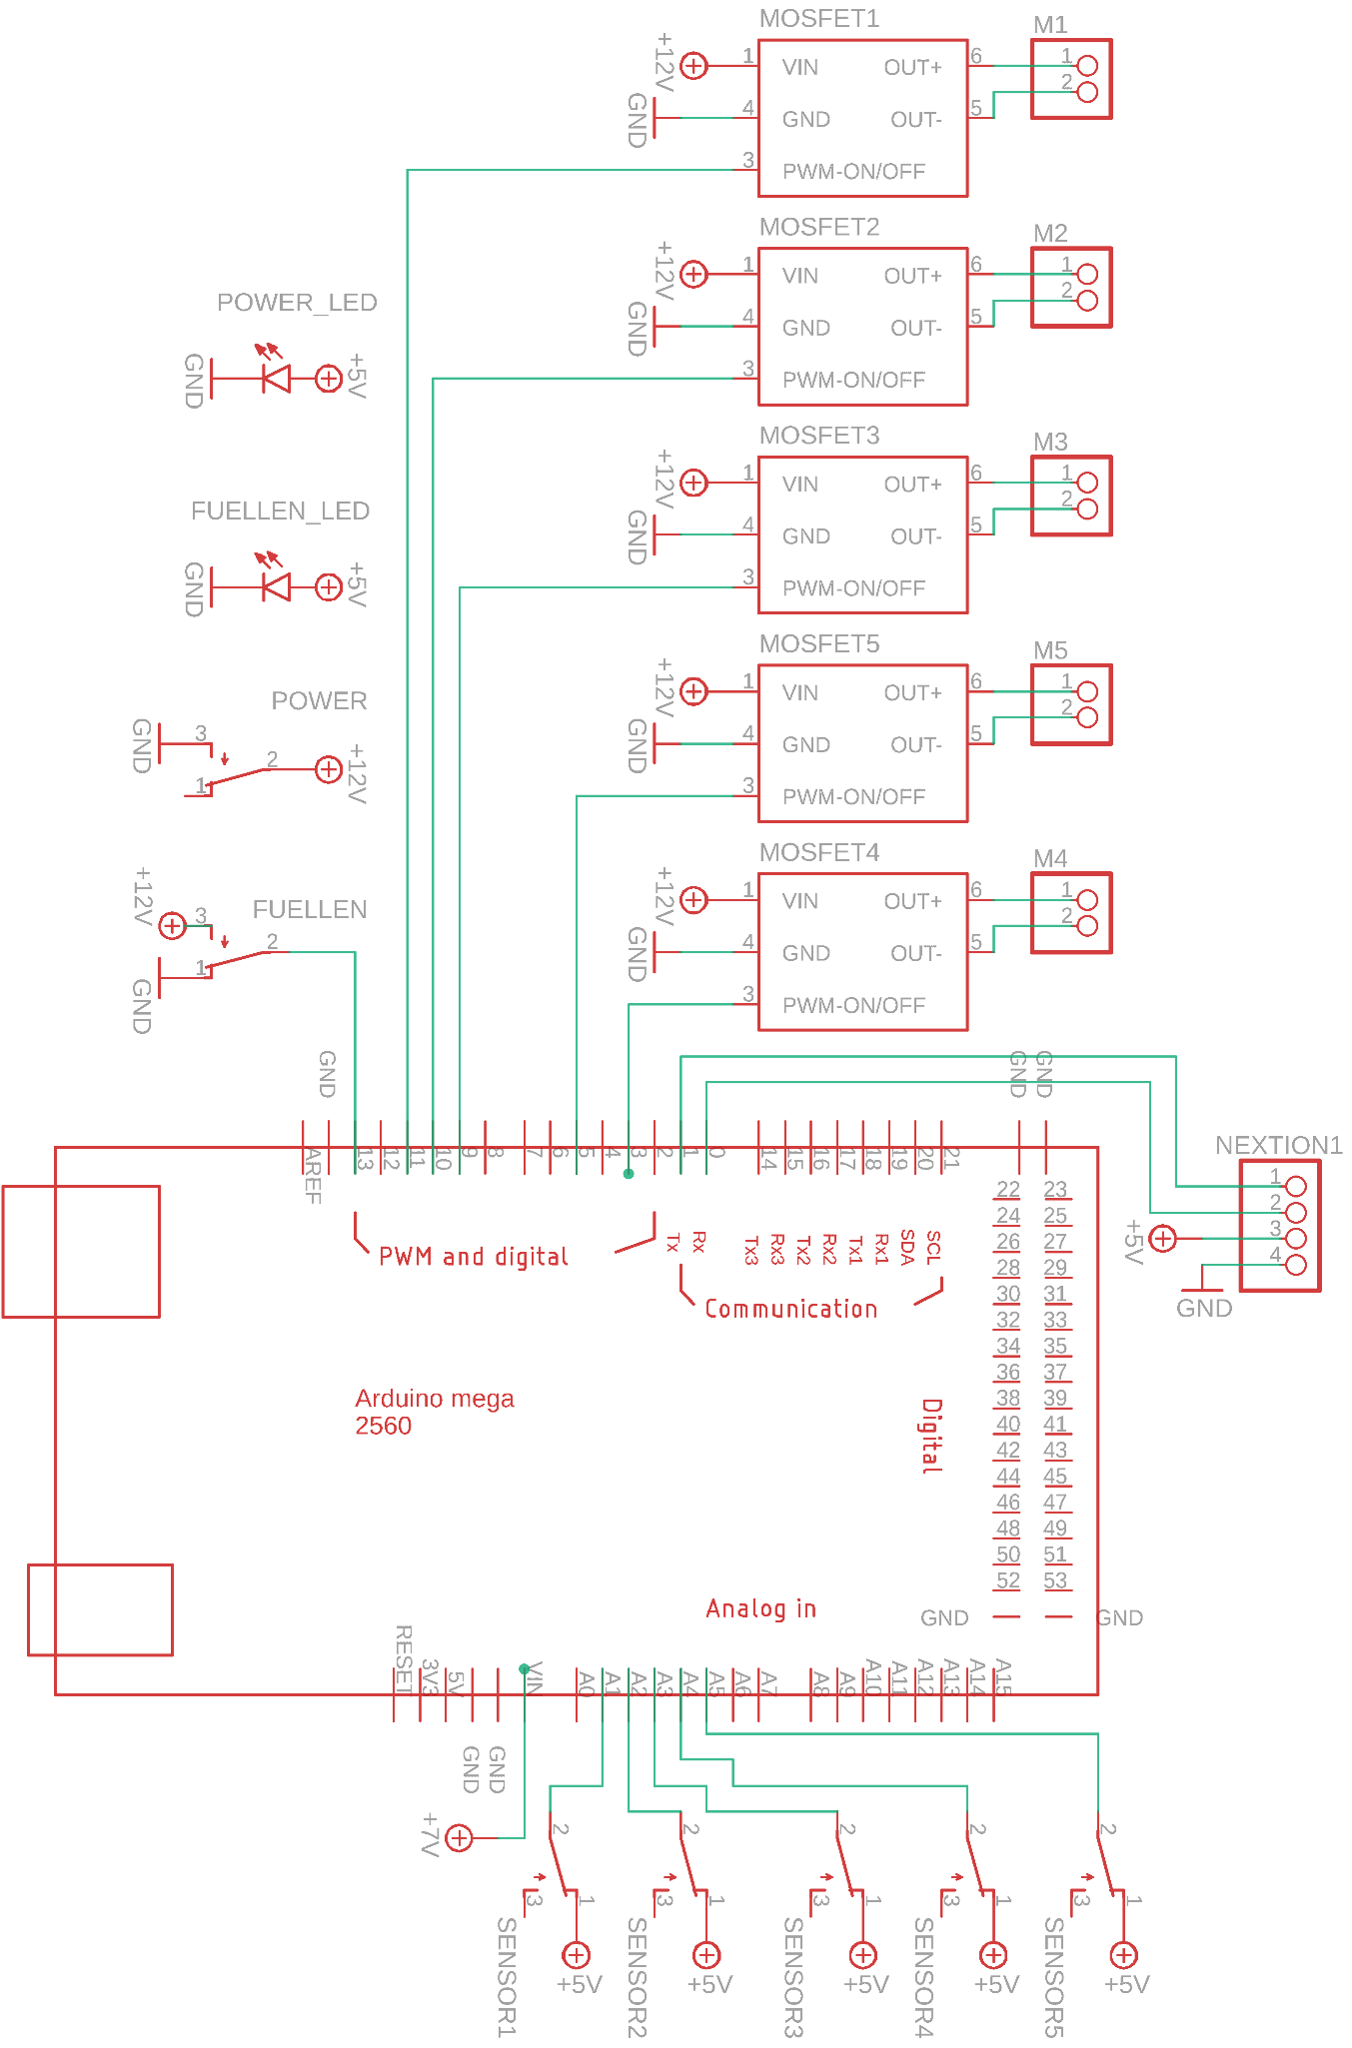
\includegraphics[angle=90, width=\textwidth]{./img/Anhang/Schaltplan.png}}
    \caption{Schaltplan}
\end{figure}

\chapter{Deep Learning Modell für die Klassifizierung}\label{Anhang_E}
\lstinputlisting[language=python, style=algoBericht, basicstyle=\tiny\sffamily, captionpos=b, caption={Deep Learning Modell für die Klassifizierung}, escapeinside={\#*}{*)}]{./Listings/train_dialog_model.py}


%\addcontentsline{toc}{chapter}{Liste der ToDo's}
%\listoftodos[Liste der ToDo's]


\end{document}
